\documentclass[a4paper,12pt]{book}
\usepackage[utf8]{inputenc}
\usepackage[toc,page]{appendix}
\usepackage{amstext,amsmath,amssymb,bm,bbm,mathtools,accents}
\usepackage{graphicx,wrapfig,xcolor,subfig}
\usepackage{algorithm2e}
\usepackage{float}
\usepackage{listings}
\usepackage{rotating}
\usepackage{enumitem}
\usepackage{array,multirow}
\usepackage{chronosys}
\usepackage{geometry}
\usepackage[hidelinks,colorlinks]{hyperref}
\usepackage[noabbrev,capitalise,nameinlink]{cleveref}
\usepackage{pdflscape}
\usepackage{afterpage}
\usepackage{longtable}
\usepackage{layouts}
\usepackage[export]{adjustbox}


%\usepackage{natbib}
%\bibliographystyle{alpha}
\usepackage[style=alphabetic,maxbibnames=99,backref=true]{biblatex}
\addbibresource{thesis.bib}


\setlength{\oddsidemargin}{0.5cm}
\setlength{\evensidemargin}{0.5cm}
\setlength{\marginparwidth}{0.5cm}

\setlength{\marginparpush}{0cm}
\setlength{\marginparsep}{0cm}
\setlength{\columnsep}{0pt}

\setlength{\textwidth}{14.92cm} %21cm - 2in -1cm (2in for the standard horizontal offset; 1in for each side)

\widowpenalty10000
\clubpenalty10000

\newcommand{\daniel}[1]{{\color{red}{#1}}}

\newcounter{definition}[section]
\newenvironment{definition}[1]{\refstepcounter{definition} \par\bigskip \noindent  \begin{minipage}[b]{\linewidth} 
\textbf{Definition~\thedefinition(#1):}}{\end{minipage} \par\bigskip}

\newcounter{example}[section]
\newenvironment{example}{\refstepcounter{example} \par\medskip
\noindent  \textbf{Example~\theexample :}}{\medskip}


\newcounter{claim}[section]
\newenvironment{claim}[1]{\refstepcounter{claim} \par\medskip \noindent  \textbf{Claim~\theclaim(#1):}}{\medskip}

\newcounter{lemma}[section]
\newenvironment{lemma}{\refstepcounter{lemma} \par\medskip \noindent  \textbf{Lemma~\thelemma:}}{\medskip}


\newcounter{proposition}[section]
\newenvironment{proposition}[1]{\refstepcounter{proposition} \par\medskip \noindent  \textbf{Proposition~\theproposition(#1):}}{\medskip}

\newcounter{theorem}[section]
\newenvironment{theorem}[1]{\refstepcounter{theorem} \par\medskip \noindent  \textbf{Theorem~\thetheorem(#1):}}{\medskip}


\newcounter{assumption}[section]
\newenvironment{assumption}{ \refstepcounter{assumption} \renewcommand{\theequation}{A.\arabic{assumption}} }{\renewcommand{\theequation}{\arabic{section}.\arabic{equation}}}


\crefname{algocf}{alg.}{algs.}
\Crefname{algocf}{Algorithm}{Algorithms}
\Crefname{appsec}{Appendix}{Appendices}



\DeclareMathOperator*{\argmin}{arg\,min}
\DeclareMathOperator*{\argmax}{arg\,max}
\renewcommand{\vec}[1]{\bm{#1}}
\DeclarePairedDelimiter\norm{\lVert}{\rVert}%
\DeclarePairedDelimiter\bignorm{\Big\lVert}{\Big\rVert}%
\DeclarePairedDelimiter\abs{\lvert}{\rvert}%

\newcommand{\edge}[2]{ ( \overrightarrow{ #1,#2} )}

\newcommand{\sketch}[1]{{\color{red}{#1}}}
\newcommand{\ol}[1]{{\overline{#1}}}
\newcommand{\av}[1]{\accentset{\circ}{\vec{#1}}}
\newcommand{\Ds}{D}
\newcommand\figTable[2]{\raisebox{-.5\height}{\includegraphics[scale=#1]{#2}}}

\newcommand{\transp}{\mathbf{T}}
\newenvironment{proof}{\noindent\ignorespaces\textit{Proof: }}{\hfill $\blacksquare$ \par\noindent\ignorespacesafterend\medskip}

\makeatletter
\DeclareFontFamily{U}{tipa}{}
\DeclareFontShape{U}{tipa}{m}{n}{<->tipa10}{}
\newcommand{\arc@char}{{\usefont{U}{tipa}{m}{n}\symbol{62}}}%

\newcommand{\arc}[1]{\mathpalette\arc@arc{#1}}

\newcommand{\arc@arc}[2]{%
  \sbox0{$\m@th#1#2$}%
  \vbox{
    \hbox{\resizebox{\wd0}{\height}{\arc@char}}
    \nointerlineskip
    \box0
  }%
}
\makeatother



\begin{document}
	\title{Geometric constraints and variational approaches to image analysis}
	\author{Daniel Antunes}
	\date{}
	\maketitle
	
	\begin{center} 
 \textbf{Abstract}
\end{center}

Several problems in image processing belong to the class of inverse problems, and hypotheses should be made to have a well-defined formulation, i.e., a formulation in which a solution exists and it is unique. A possibility is to use geometric criteria to regularize the problem, e.g., to favor solutions with smooth contours or short perimeters. This process is called regularization. 

However, it is likely the case that the objects in the scene have unknown mathematical representations and that such geometric measurements should be computed in place, considering only their visual representation: In the case of image processing, a digital image. Usually, such measurements are computed without considering the nature of the digital domain, and consequently, are not guaranteed to converge neither approximate the expected Euclidean quantity. The regularization is thus incorrect or not precise, and the solutions biased.

Recently, several digital estimators of geometric properties such as tangent and curvature were proven multigrid convergent. In other words, the estimated values computed in the digital representation of a shape converges towards the values computed in its Euclidean representation as the digital mesh becomes finer and finer. However, there exist few models in the image processing literature that make use of them. That is because such estimators are more difficult to integrate in an optimization framework.

In this thesis, we investigate the use of multigrid convergent estimators and their applications in image processing. In particular, we aim to integrate regularizers based on convergent estimators of curvature in image segmentation problems. We present four combinatorial models based on the elastica energy (a classical geometric regularization term combining perimeter and curvature) with applications in image segmentation. Next, we evaluate our results and compare with similar methods. The results have shown to be very competitive with the state of art.	
	\newpage
	\begin{center} 
 \textbf{Résumé}
\end{center}

Beaucoup de problèmes en analyse d’images sont caractérisés comme des problèmes inverses, et des hypothèses s'avèrent nécessaire pour obtenir un formulation bien posée, c’est-à-dire que le problème ait une solution et que celle-ci soit unique. Une approche possible consiste à utiliser des critères géométriques pour régulariser le problème, par exemple pour favoriser des solutions avec des contours lisses ou de faible périmètre. 

Cependant, dans le cadre de l’analyse d’image; nous ne disposons pas de la représentation mathématique des objets dans une scène observée. Nous devons utiliser les seules données discrètes (les couleurs des pixels de l’image) qui approchent ces objets et les mesures géométriques sont alors délicates. Les méthodes classiques prennent peu en compte la nature discrète des données dans leur mesure. En conséquence, nous n’avons pas de garanties de convergence ou même d’approximation des mesures effectuées par rapport aux mesures euclidiennes attendues. La régularisation dans le processus de traitement d’image est alors incorrecte ou peu précise, et les solutions trouvées sont alors biaisées.

Récemment, plusieurs estimateurs discrets de propriétés géométriques, notamment liés à la longueur, à la tangente et à la courbure, ont été prouvé convergents multigrilles. Autrement dit la valeur mesurée par ces estimateurs sur la représentation discrète d’une forme converge vers la valeur mesurée sur sa forme euclidienne quand on utilise des grilles de discrétisations de plus en plus fines. Néanmoins, on constate que la littérature d’analyse d’image comporte peu de modèles qui utilisent des estimateurs convergents multigrille. Cela vient du fait qu’il est plus difficile des les intégrer dans les algorithmes de résolution.

Dans cette thèse, nous explorons l’utilisation d’estimateurs convergents multigrille dans des applications en analyse d’image. Plus spécifiquement nous cherchons à intégrer des régularisations basées sur des estimateurs convergents de courbure dans des processus de segmentation d’image. Nous présentons quatre modèles variationnels combinatoires basés sur l’énergie dite “Elastica” (combinaison classique de régularisation géométrique utilisant la longueur et la courbure) avec application en segmentation d’image. Nos résultats sont ensuite évaluées et comparées avec des méthodes similaires, et nos modèles s’avèrent très compétitifs avec l’état de l’art.

	
%	\setlength{\abovedisplayskip}{10pt}
%	\setlength{\belowdisplayskip}{10pt}
	
	\tableofcontents	
	\chapter{Notation}
\label{chapter:notation}

\[
\begin{array}{ll}
\mathbb{B}: & \{0,1\}\\
\mathbb{U}: & [0,1]\\
\mathbb{Z}: & \text{Integers}\\
A,B,C,D: & \text{Sets}\\
\mathbf{A,B,C,D}: & \text{Matrices}\\
\mathbf{A}_i: & \text{$i$th row vector of matrix $\mathbf{A}$}\\
\mathbf{A}_j: & \text{$j$th column vector of matrix $\mathbf{A}$}\\
\mathbf{A}_{i,j}: & \text{Element in the $i$th row and $j$th column of matrix $\mathbf{A}$}\\
X,Y,Z: & \text{Set of variables}\\
x,y,z: & \text{Scalar variables}\\
\mathbf{x,y,z}: & \text{Vector variables}\\
\mathbf{x}_i: & \text{$i$th coefficient of vector $\mathbf{x}$}\\
f,g,h: & \text{Functions}\\
\hat{f}: & \text{Estimation function}\\
\hat{\mathbf{Q}}: & \text{The filter matrix of $\mathbf{q}$}\\
\mathbbm{1}_A: & \text{Active vector for set $A$}\\
\mathbf{L}: & \text{Linel incidence matrix}\\
\partial_{dig} D: & \text{Digital boundary of a digital set $D$}
\end{array}
\]

	\chapter{Introduction}\label{chapter:introduction}
Our main object of study is the function $\mathcal{I}:\Omega \subset \mathbb{Z}^j \rightarrow [0,1]^k$. We have a grayscale digital image for $(j=2,k=1)$ and a three dimensional colored object for $(j=3,k=3)$ if we assume the RGB color scheme. Such objects are created by sampling a continuous domain and its quality is directly related with its resolution, or the number of samples one uses to discretize the domain. 

Digital image processing has been developed since the 60s, but still an active field of research. Among the reasons, we can cite the advances in acquisition, which exponentially increases the amount of data to be treated; and the popularization of digital cameras. In fact, applications involving digital images are numerous. An autonomous vehicle must partition the frames coming from its camera in meaningful regions in order to identify roads, traffic signs, people, landscape and other vehicles (segmentation); satellite images are usually degraded due to limitations in transmission and storage devices and should be processed to enhance quality (denoising); in cinema, post-production editors might be faced with undesired objects in the scenes as cables or cameras that should be removed smoothly (inpainting). 

The classical approach consists to solve an optimization problem. It is a reasonable strategy, as we are interested to find the best segmentation or the best image inpainting, the definition of best being application-based. Using information or assumptions intrinsic to the problem, we can make use of prior terms to guide the optimization process, as for example, the geometry of objects we wish to segment. In chapter \ref{chapter:regularization} we describe some classical models in image segmentation and the role of geometric priors.

The curvature is an example of geometric prior with properties that makes it suitable for the segmentation of long and thin structures as blood vessels. Its use and the difficulties that come along with it are discussed in chapter \ref{chapter:curvature-prior}, which sets the ground for our digital approach. In chapter \ref{chapter:digital-geometry} we introduce some concepts of digital geometry, among them the multigrid convergence of a digital estimator. The goal of this chapter is to argue that multigrid convergent estimators of curvature should be preferred when computing curvature in digital data. 

Finally, we describe the main product of this work in chapter \ref{chapter:digital-flow} and illustrate its results with several experiments and comparisons. In the appendix, the reader can found three other models developed during this thesis and considered relevant by the author for future investigation in the subject.

	\part{Image Processing and Digital Geometry}
%	\chapter{Variational methods in Image Processing}
\label{chapter:variational-methods-in-image-processing}

\section{Inverse problems}
%In the music world, nothing is as complex as an orchestra score. You have plenty of instruments following different tones, dynamics, intensities, rhythms and so on. But no matter the complexity, given the orchestra score a software can reproduce with perfection the piece of music. It is a totally  different story if you ask it to create the orchestra score from an audio file. Reading the score is a forward problem, and creating the score is an inverse problem.

An archaeological museum decided to digitize all its collection and make them available for digital visits over the internet. The chosen method of digitization consists into take a set of pictures, in different camera positions, for each object and then to use a stereo algorithm to assemble all the pieces and create a 3D model of the object. The stereo problem is an \emph{inverse problem}.

Inverse problems are characterized by a degree of \emph{uncertainty} or \emph{lack of information}. The 2D pictures in the problem above miss depth information, that should be \emph{inferred} by the stereo algorithm. On the other hand, if the shape geometry was known, e.g., the values of mean curvature were known for every infinitesimal point of the shape, then constructing a digital 3D representation would be a \emph{forward problem}. 

Inverse problems are ubiquitous in science. We can find inverse problems in several branches of mathematics~\cite{kirsch96}, geophysics~\cite{zhdanov15}, natural language processing~\cite{stroppa05}, astronomy~\cite{lucy94} and the list goes on. The image processing field itself field is plenty of examples of inverse problems~\cite{bertero98}, some of them listed in table~\cref{ch1:tab:inverse-problems-list}. In fact, a great part of real world applications consists into infer parameters of some model, i.e., an inverse problem. In~\cref{ch1:tab:inverse-problems-list} we list some examples of inverse problems and its corresponding direct problem version.

\begin{table}
\renewcommand{\arraystretch}{1.5}
\footnotesize
\begin{tabular}{|m{7cm}|m{7cm}|}
\hline
\multicolumn{1}{|c|}{\textbf{Inverse problem}} & \multicolumn{1}{c|}{\textbf{Forward problem}} \\
\hline
\textbf{Projection}: Compute vector $v \in \mathbb{R}^3$ which projection is $P(v) \in \mathbb{R}^2$ & Compute the projection $P(v) \in \mathbb{R}^2$ of vector $v \in R^3$\\
\hline
\textbf{Parameters inference}: Given a set of observations $\Gamma$, infer the parameters $(\mu,\sigma)$ of the Gaussian distribution that describes $\Gamma$ & Given a random variable $X$ following a Gaussian distribution with parameters $(\mu=0,\sigma=1)$, compute the probability $P(X \leq 0.42)$\\
\hline
\textbf{Image denoising}: Given noisy image $\widetilde{\vec{I}}$, compute the original image $\vec{I}$, i.e., the image without noise & Add some random noise to a given image $\vec{I}$ to produce noisy image $\widetilde{\vec{I}}$\\
\hline
\textbf{Image inpainting}: Given image $\widetilde{\vec{I}}$ with a missing patch, reconstruct the removed patch & Remove a patch from image $\vec{I}$ \\
\hline
\textbf{Image segmentation}: Given image $I$, find the labeled partition $\mathcal{I}$ & Given a labeled partition $\mathcal{I}$ of some image $I$, assemble the pieces to create image $I$\\
\hline
\end{tabular}
\caption{Examples of inverse problems and its direct versions. Inverse problems are characterized by uncertainty and parameter inference. }
\label{ch1:tab:inverse-problems-list}
\end{table}

In mathematics, uncertainty is very often translated in to ill-posed problems. An ill-posed problem is a problem that is not well-posed. A well-posed problem, on the other hand, must respect the two conditions below.

\begin{enumerate}
\item{A solution exists and it is unique;}
\item{The solution changes continuously with its parameters}
\end{enumerate}



Generally speaking, an inverse problem is ill-posed. In order to solve ill-posed problems one should include additional information, i.e., create assumptions over the properties of searched solution. For example, one may assume that vector $v$ is at some distant $d$ of $P(v)$ for the projection problem. The solution set, in this case, is restricted to two. The process of including additional information in ill-posed problems is called \emph{regularization} and its goal is to transform ill-posed problems in well-posed ones. 

\section{Image model}
As remarked in the previous section, inverse problems involve some level of uncertainty about the solution. In order to solve an ill-posed problem we need to regularize it by including additional information, or assumptions. To simplify notation, we limit our discussion to grayscale images, the concepts being extendable to multichannel images. It is convenient to have in mind two different representations of an image. \\

\begin{center}
\begin{tabular}{rl}
	Continuous: & $f_I: \Omega \subset \mathbb{R}^2 \rightarrow \mathbb{U}$ \\
	Discrete: & $I \in \mathbb{F}^{m \times n}$,
\end{tabular}
\end{center}

where $\mathbb{F}$ is a finite set. In this thesis, we define such set as

\begin{align}
	\mathbb{F} &= \{ \frac{i}{255} \; | \; i \in \mathbb{N}, i \leq 255 \}.
\end{align}

The discrete representation is interpreted as a sampling of $m \times n$ elements (pixels) of the continuous function $f_I$. 

\section{Image denoising}

Given a corrupted image $\vec{\widetilde{I}}$, the image denoising problem consists in to recover the uncorrupted image $\vec{I}$.

\subsection{Bayesian rationale}
The maximum a posteriori method was first introduced in the image processing community in the work of~\cite{geman84}. We reproduce it here the rational for image denoising.

Image denoising is an inverse problem and we need to make some assumptions in order to advance in its solution. As our first assumption, we assume that the corrupted image $\widetilde{\vec{I}}$ is the result of summing the original image $\vec{I}$ to a $(m \times n)$ matrix $\vec{N}$ of random variables $\vec{N}_{i,j}$ following a normal Gaussian distribution, i.e, 

\begin{align}
	\vec{\widetilde{I}} &= \vec{I} + \vec{N},
	\label{ch1:eq:gaussian-noise-model}
\end{align} 

where $Pr\big( \vec{N}_{i,j} = n \big) = \frac{1}{\sqrt{2\pi}}exp( \frac{n^2}{2} )$. If we want to be precise, the sum operator in~\cref{ch1:eq:gaussian-noise-model} should be redefined to be a closed operator in $\mathbb{F}^{m \times n}$. We skip this definition by arguing that because of the symmetry of the Gaussian distribution the computation of the probabilities that follows remains the same.

 We are going to estimate the original image $\vec{I}$ as the image $\vec{I}^{\star}$ that is more likely to occur following~\cref{ch1:eq:gaussian-noise-model}, i.e., 

\begin{align}
	\vec{I}^{\star} & = \argmax _{\vec{C}}{Pr(\vec{C} \; | \;\vec{\widetilde{I}})} = \argmax _{\vec{C}} \frac{Pr(\vec{\widetilde{I}} \; | \; \vec{C})Pr(\vec{C})}{Pr(\vec{\widetilde{I}})},
	\label{ch1:eq:probability-maximization}
\end{align}

where the last expression was derived by applying Bayes' theorem. From~\cref{ch1:eq:gaussian-noise-model} we derive the probability of having the corrupted image $\vec{\widetilde{I}}$ given the original image $\vec{I}$, i.e.,

\begin{align}
	Pr(\vec{\widetilde{I}} \; | \; \vec{C}) &= Pr( \vec{N} = \vec{\widetilde{I}} - \vec{C} ) = \frac{1}{\sqrt{2\pi}}exp\Big(- \frac{ \norm{\vec{\widetilde{I}} - \vec{C} }^2}{2} \Big).
	\label{ch1:eq:probability-corrupted-image-given-original}
\end{align}

Next, we make our second assumption. We are going to favor candidate images that respect some desirable property for the problem to be solved. A popular one for denoising is to assume that the image is piecewise smooth, i.e., its made of closed regions of smooth variations in the color intensity in its interior but with strong discontinuities in their boundaries. There are several ways to model this property. For the moment, let's simply assume that $Pr(\vec{C}) = exp\big(-\rho(\vec{C})\big)$. The denominator term in~\cref{ch1:eq:probability-maximization} is computed as

\begin{align*}
	Pr(\widetilde{\vec{I}}) &= \sum_{\vec{J} \in \mathbb{F}^{m \times n}}{Pr(\vec{\widetilde{I}}\;|\; \vec{J})Pr(\vec{J})} = \frac{1}{\sqrt{2 \pi}}\sum_{\vec{J} \in \mathbb{F}^{m \times n}}{exp\bigg(-\frac{1}{2}\norm{\widetilde{\vec{I}}-\vec{J}}^2 - \rho(\vec{J})}\bigg).
\end{align*}

and~\cref{ch1:eq:probability-maximization} is expanded as

\begin{align}
	\vec{I}^{\star} & = \argmax _{\vec{C}} \frac{1}{\sqrt{2\pi}} \frac{exp\Big(- \frac{1}{2}\norm{\vec{\widetilde{I}} - \vec{C}}^2 - \rho(\vec{C}) \Big) }{ \sum_{\vec{J} \in \mathbb{F}^{m \times n}}{exp\bigg(-\frac{1}{2}\norm{\widetilde{\vec{I}}-\vec{J}}^2 - \rho(\vec{J})}\bigg) }
	\label{ch1:eq:probability-maximization-expanded}
\end{align}

Finnaly, solving~\cref{ch1:eq:probability-maximization-expanded} is equivalent to solve

\begin{align}
	\vec{I}^{\star} &= \argmin _{\vec{C}} \frac{1}{2}\norm{\vec{\widetilde{I}} + \vec{C}}^2 + \rho(\vec{C}).
	\label{ch1:eq:minimization-form}
\end{align}

The first term appears so often in image processing that it has a special name: \emph{data fidelity}. In the denoising problem, the data fidelity term appeared as a consequence of the Gaussian noise model assumption. The second term is also a regularization term, in this case modeling our assumption that the original image is piecewise smooth. We can follow this reasoning for each new assumption we made. The consequence being an additional term in~\cref{ch1:eq:minimization-form}.

\subsection{Tikhonov regularization}

The classical way to optimize~\cref{ch1:eq:minimization-form} is to shift it to a continuous setting, analytically derive optimization properties and then use this properties to solve the problem in a discrete setting. The continuous reformulation of~\cref{ch1:eq:minimization-form} consists in to optimize the energy functional below

\begin{align}
	f_{I^{\star}} &= \argmin_{f} F(f) = \frac{1}{2} \int_{\Omega}{ \norm{ f_{\widetilde{I}} - f}^2dx} + R(f),
	\label{ch1:eq:variational-formulation}
\end{align}

where $R$ is a functional derived from the choice of $\rho$. A popular choice for $R$ is to define it as the $L2$ norm of $\nabla f$, also called the \emph{Tikhonov term}.~\cref{ch1:eq:variational-formulation} is rewritten as

\begin{align}
	f_{I^{\star}} &= \argmin_{f} F(f) = \frac{1}{2} \int_{\Omega}{ \norm{ f_{\widetilde{I}} - f}^2dx} + \int_{\Omega}{ \norm{ \nabla f }^2 dx }.
	\label{ch1:tikhonov-formulation}
\end{align}

\subsubsection{Euler-Lagrange equation}

We can establish some necessary optimization conditions for~\cref{ch1:tikhonov-formulation} by deriving its Euler-Lagrange equation. Assume that function $g$ minimizes functional $F$, i.e.,

\begin{align*}
	g &= \argmin_{f}{F(f)}.
\end{align*}

Further, assume that there exists a function $w$ such that $w(x)=0,\, \forall x \in \partial \Omega$. Define the function $h$ as

\begin{align*}
	h(\epsilon) &= F(g+\epsilon w)
\end{align*}

Therefore, $h$ achieves an extreme value in $\epsilon=0$. Thus,

\begin{align*}
	0 = \frac{dh}{\partial \epsilon}_{| \epsilon=0} &= \frac{d}{\partial \epsilon}_{| \epsilon=0} \frac{1}{2} \int_{\Omega}{ \norm{f_{\widetilde{I}} - g - \epsilon w}^2 + \norm{ \nabla (g + \epsilon w) }^2} \\
	&= _{| \epsilon = 0} \frac{1}{2} \int_{\Omega}{ 2\norm{f_{\widetilde{I}} - g - \epsilon w}\frac{(f_{\widetilde{I}} - g - \epsilon w) }{\norm{f_{\widetilde{I}} - g - \epsilon w}}w + 2\norm{ \nabla (g + \epsilon w) }\frac{(\nabla g + \epsilon w)}{\norm{ \nabla (g + \epsilon w) }}\nabla w} \\
	&= \int_{\Omega}{ (f_{\widetilde{I}} - g)w + (\nabla g)\nabla w}. 	
\end{align*}

Applying integration by parts and using the fact that $w(x)=0,\; \forall x \in \partial \Omega$.

\begin{align*}
		0 &= \int_{\Omega} ( f_{\widetilde{I}} - g - \Delta g )w
\end{align*}

Since $w$ could be any function, we can write

\begin{align}
	f_{\widetilde{I}} - g - \Delta g &= 0
	\label{ch1:eq:variational-necessary-condition}
\end{align}


Therefore, if $g$ is a minimum of~\cref{ch1:eq:variational-formulation}, then it respects ~\cref{ch1:eq:variational-necessary-condition}. ~\cref{ch1:eq:variational-formulation} can be proven to be convex. Hence, given an initial solution $f$, one can execute a descent method (gradient descent, for example) to find the minimum of~\cref{ch1:eq:variational-formulation}. In practice, ~\cref{ch1:eq:variational-formulation} is discretized using the samplings $I,\widetilde{I}$ of $f_I,f_{\widetilde{I}}$ and a finite differences scheme is defined to estimate the Laplacian $\Delta$.

The Tikhonov term favors images with smooth variations in color, but the smoothness is not restricted to the interior of regions. Thus, Tikhonov tends to obfuscate the discontinuities set and the image appears to be blurred (see~\cref{ch1:fig:denoising-results}). Nonetheless, Tikhonov term is attractive due to its optimization properties.


\subsection{Total variation regularization}
An alternative to Tikhonov regularization is to use the so called total variation of the image function. The problem to be minimized is then defined as

\begin{align}
	f_{I^{\star}} &= \argmin_{f} \frac{1}{2} \int_{\Omega}{ \norm{ f_{\widetilde{I}} - f}^2dx} + \int_{\Omega}{ \norm{\nabla f} dx}.
\end{align}

The $L1$ norm favors smooth interiors and it is less aggressive in the boundaries. Moreover, there are efficient algorithms to solve it~\cite{rudin92,chambolle04,beck09}.

\begin{figure}
\subfloat[Original]{
\includegraphics[scale=0.38]{figures/chapter2/denoising/coala-original.png}
}%
\subfloat[Noisy]{
\includegraphics[scale=0.38]{figures/chapter2/denoising/coala-noise.png}
}%
\subfloat[Tikhonov]{
\includegraphics[scale=0.38]{figures/chapter2/denoising/coala-tikhonov.png}
}%
\subfloat[Total Variation]{
\includegraphics[scale=0.38]{figures/chapter2/denoising/coala-chambolle.png}
}%
\caption{Denoising algorithms results for the Tikhonov and Total variation regulararization terms.}
\label{ch1:fig:denoising-results}
\end{figure}

\section{Image segmentation}
\subsection{Length regularization terms}
\subsection{Mumford-Sha}
\subsection{Chan-Vese}
\subsection{Active contours}

\section{Image inpainting}
\subsection{Level sets completion}



%There is an equivalence between Gibbs distributions and MRF.
%
%Maximum a posteriori is also called penalized maximum likelihood
%
%Consider the problem to find $x$ such that $Ax=b$. If the problem has none or several solutions, the problem is said do be ill-posed. The standard method to solve it is by least-squares plus a penalty term. $|Ax-b|^2 + \lambda P$. The term $P$ models a preference for solutions with some desirable property, e.g., $P=|x|^2$ will favor solutions with lower norm.
%
%Tikhonov regularization is a type of L2 regularization. It is known to improve the problem conditioning and to enable direct solutions (wikipedia article).
%	\chapter{Discrete methods in Image Processing}
\label{chapter:discrete-methods-in-image-processing}

%\startchronology[startyear=1980,stopyear=2020, startdate=false, color=blue!40, stopdate=false, arrow=true, height=3pt]
%\setupchronoevent{textstyle=\scriptsize,datestyle=\scriptsize,date=false}
%\chronograduation[event]{10}
%\chronoevent[markdepth=20pt]{1967}{\cite{viterbi67}}\chronoevent[markdepth=-20pt]{1981}{\cite{nemhauser81}}\chronoevent[markdepth=40pt]{1982}{\cite{pearl82}}\chronoevent[markdepth=-40pt]{1984}{\cite{geman84,hammer84}}\chronoevent[markdepth=60pt]{1985}{\cite{billionnet85}}\chronoevent[markdepth=-60pt]{1986}{\cite{besag86}}\chronoevent[markdepth=20pt]{1991}{\cite{boros91}}\chronoevent[markdepth=-20pt]{2001}{\cite{boykov01graphcut,boykov01fast}}\chronoevent[markdepth=40pt]{2002}{\cite{boros02pseudo}}\chronoevent[markdepth=-40pt]{2003}{\cite{boykov03geodesics,ishikawa03}}\chronoevent[markdepth=60pt]{2004}{\cite{kolmogorov04whatenergies}}\chronoevent[markdepth=-60pt]{2005}{\cite{kohli05efficiently}}\chronoevent[markdepth=20pt]{2006}{\cite{juan06active,szeliski06comparative}}\chronoevent[markdepth=-20pt]{2007}{\cite{rother07qpbo,veksler07graph}}\chronoevent[markdepth=40pt]{2008}{\cite{ramalingam08,delong08scalable,vicente08graph}}\chronoevent[markdepth=-40pt]{2009}{\cite{koller09,orlin09faster}}\chronoevent[markdepth=60pt]{2010}{\cite{ishikawa10}}\chronoevent[markdepth=-60pt]{2011}{\cite{blake11markov}}\stopchronology

In the beginning of the last chapter we described the Bayesian rational for the denoising problem. We turn once again to probability thinking, but restricting our analysis to discrete probabilistic models. Markov Random Fields are in the conception of the methods discussed in this chapter, and an inspiration for many others. Image pixels are naturally interpreted as Markov states, and image properties, as spatial coherence, are encoded as potentials stored in the edges of the image grid graph. The MAP inference boils down to minimize the challenging class of pseudo-boolean functions. 

In some fortunate cases, the functions can be minimized exactly and efficiently by a reduction to a max-flow (min-cut) problem, and it happens that such cases model imaging problems, as segmentation, nicely well. In fact, the minimum cut defines a partition, and one can interpret the cut as the contour separating two objects. It is the key for fruitful research that has followed. One can abstract the MRF machinery and define potentials on vertices and edges of the grid graph such that its minimum cut answers the problem being posed. Moreover, the potentials can model geometric properties of objects embedded in the grid graph, and one can use cuts to estimate the objects perimeters, for example.

We start this chapter by giving a brief description of Markov Random Fields and the minimization problem arising from the MAP inference. In the second section we present some properties of pseudo-boolean functions and how to optimize them. In the third section we describe the special class of submodular functions and efficient algorithms to compute the minimum of such functions. Finally, we describe successful models in the image processing community based on graph cuts and how one can inject geometric information on them.


\section{Markov Random Fields}
\label{ch2:sec:markov-random-fields}

Let $\mathcal{G}=(\mathcal{V},\mathcal{E})$ an undirected graph with vertices set $\mathcal{V}$ and edges set $\mathcal{E}$. The set of adjacent vertices to $v \in V$ is denoted $\mathcal{N}(v)$. Given two subsets $S,Q \subset \mathcal{V}$, a $(S,Q)$-cut is any subset of edges $\mathcal{E}' \subset \mathcal{E}$ such that $S,Q$ are in different connected components in the graph $\mathcal{G}(\mathcal{V},\mathcal{E} \setminus \mathcal{E}')$. We denote $cut(S,Q)$ the set of all $(S,Q)$ cuts.

For each vertex $v \in \mathcal{V}$ we associate a discrete random variable $X_v$ that take values from a label set $\Gamma_v$ according with some distribution $P$. We group all random variables in vector $\vec{X}$ and we write $\vec{X}_S$ to refer to the set of associated variables with vertex set $S \subset \mathcal{V}$. We also group all the label sets in the collection $\Gamma$. We denote $W_{\vec{X}}$ the set of all configurations for the random vector $\vec{X}$. We say that $\mathcal{H} =(\mathcal{G},\vec{X},\Gamma,P)$ is a \emph{Markov Random Field} (MRF) if for any non-adjacent states $X_u$ and $X_v$, the probability distribution $P$  satisfies the independence conditions below
\begin{align}
	\textbf{Pairwise independencies:}&\quad \Big\{ X_u \perp X_v \;|\; \big\{X_i,\; \forall i \in \mathcal{V}\setminus\{u,v\} \big\}  \Big\} \label{ch2:eq:markov-pairwise-independencies}   \\
	\textbf{Local independencies:}&\quad \Big\{ X_u \perp X_v \;|\; \big\{X_i, \; \forall i \in \mathcal{N}(u)  \big\} \Big\} \label{ch2:eq:markov-local-independencies} \\
	\textbf{Global independencies:}& \quad \Big\{ \vec{X}_S \perp \vec{X}_Q \;|\; \vec{X}_Z,\; \text{where } \vec{X}_Z \in cut(S,Q) \Big\} \label{ch2:eq:markov-global-independencies},
\end{align}
%
where $X_u  \perp  X_v \;|\; \vec{X}_S$ means that variable $X_u$ is independent of $X_v$ given an assignment of variables in $\vec{X}_S$.  For example, the MRF in~\cref{ch2:fig:example-mrf} respects the following expressions 
\begin{align*}
		P\Big(X_1=w_1 \; | \big\{X_i=w_i, \, i \neq 1 \big\} \Big) &= P\Big(X_1=w_1 \; | \; X_2=w_2,X_3=w_3 \Big) \\
		P\Big(X_3=w_3 \; | \big\{X_i=w_i, \, i \neq 3 \big\} \Big) &= P\Big(X_3=w_3 \; | \; X_1=w_1,X_2=w_2, X_4=w_4 \Big) \\
		P\Big(\vec{X}_{C_{123}} = \vec{w} \; | X_4=w_4, X_5=w_5  \Big) &= P\Big(\vec{X}_{C_{123}} = \vec{w} \; | \; X_4=w_4 \Big),		
\end{align*}
%
where we use the shorter notation $\vec{X}_{C_{123}} = \vec{w} $ to denote some assignment of the random variables associated with the nodes of clique $C_{123}$. A clique is any complete subgraph of $\mathcal{G}$. Given a graph, it may be quite difficult to sort out a probability distribution that satisfies~\cref{ch2:eq:markov-pairwise-independencies,ch2:eq:markov-local-independencies,ch2:eq:markov-global-independencies}. However, for the class of MRF that can be \emph{factorized} in terms of the maximal cliques of $\mathcal{G}$, creating a valid probability distribution is straightforward with the help of \emph{clique potential} functions.

\begin{figure}
\center
\begin{minipage}{0.3\textwidth}
\includegraphics[scale=0.10]{figures/chapter2/mrf/mrf-example.png}
\end{minipage}%
\begin{minipage}{0.35\textwidth}
\tiny
\begin{tabular}{|c|c|c|c|c|l|}
\hline
\multicolumn{5}{|c|}{$\omega$} & \\
\hline
$X_1$ & $X_2$ & $X_3$ & $X_4$ & $X_5$ & $P(\omega)$\\
\hline
0 & 0 & 0 & 0 & 0 & 0.0238 \\
0 & 0 & 0 & 0 & 1 & 0.0023 \\
0 & 0 & 0 & 1 & 0 & 0.0011 \\
0 & 0 & 0 & 1 & 1 & 0.0059 \\
0 & 0 & 1 & 0 & 0 & 0.0238 \\
0 & 0 & 1 & 0 & 1 & 0.0023 \\
0 & 0 & 1 & 1 & 0 & 0.0011 \\
0 & 0 & 1 & 1 & 1 & 0.0059 \\
0 & 1 & 0 & 0 & 0 & 0.119 \\
0 & 1 & 0 & 0 & 1 & 0.0119 \\
0 & 1 & 0 & 1 & 0 & 0.0059 \\
0 & 1 & 0 & 1 & 1 & 0.0297 \\
0 & 1 & 1 & 0 & 0 & 0.0476 \\
0 & 1 & 1 & 0 & 1 & 0.0047 \\
0 & 1 & 1 & 1 & 0 & 0.0023 \\
0 & 1 & 1 & 1 & 1 & 0.0119 \\
\hline
\end{tabular}
\end{minipage}%
\begin{minipage}{0.35\textwidth}
\tiny
\begin{tabular}{|c|c|c|c|c|l|}
\hline
\multicolumn{5}{|c|}{$\omega$} &\\
\hline
$X_1$ & $X_2$ & $X_3$ & $X_4$ & $X_5$ & $P(\omega)$\\
\hline
1 & 0 & 0 & 0 & 0 & 0.119 \\
1 & 0 & 0 & 0 & 1 & 0.0119 \\
1 & 0 & 0 & 1 & 0 & 0.0059 \\
1 & 0 & 0 & 1 & 1 & 0.0297 \\
1 & 0 & 1 & 0 & 0 & 0.0476 \\
1 & 0 & 1 & 0 & 1 & 0.0047 \\
1 & 0 & 1 & 1 & 0 & 0.0023 \\
1 & 0 & 1 & 1 & 1 & 0.0119 \\
\textbf{1} & \textbf{1} & \textbf{0} & \textbf{0} & \textbf{0} & \textbf{0.238} \\
1 & 1 & 0 & 0 & 1 & 0.0238 \\
1 & 1 & 0 & 1 & 0 & 0.0119 \\
1 & 1 & 0 & 1 & 1 & 0.0595 \\
1 & 1 & 1 & 0 & 0 & 0.0952 \\
1 & 1 & 1 & 0 & 1 & 0.0095 \\
1 & 1 & 1 & 1 & 0 & 0.0047 \\
1 & 1 & 1 & 1 & 1 & 0.0238 \\
\hline
\end{tabular}
\end{minipage}
\caption{\textbf{Example of a Markov Random Field}. The nodes $X_1, X_2, X_3$ forms the $3$-clique $C_{123}$.}
\label{ch2:fig:example-mrf}
\end{figure}

\subsection{Clique factorization and Gibbs energy}

A distribution $P_{\Phi}$ is a \emph{Gibbs distribution} if it can be parameterized by a set of factors $\Phi = \{\phi_1,\phi_2,\dots \phi_m\}$, i.e., 
\begin{align*}
	P_{\Phi}(\vec{X} = \vec{w}) &= \frac{1}{Z}\prod_{i=1}^{m}{\phi_i(\vec{w})} \\
	Z &= \sum_{\vec{w} \in W_{\vec{X}}}{ \prod_{i=1}^{m}{\phi_i(\vec{w})} }
\end{align*}
%
%
For strictly positive distributions ($P(\vec{X} = \vec{w}) > 0\; \forall \vec{w} \in W_{\vec{X}}$), the \emph{Hammersley-Clifford} theorem~\cite{koller09} states that $(\mathcal{G},\vec{X},\Gamma,P)$ is a MRF if and only if $P$ is a Gibbs distribution parameterized over complete subgraphs (cliques) of $\mathcal{G}$. Therefore, for MRF with strictly positive distributions $P$ we can write 
\begin{align}
	P(\vec{X} = \vec{w}) &= \frac{1}{Z}\prod_{c \in \mathcal{C}}{\phi_c(\vec{w})} \label{ch2:eq:gibbs-distribution}\\
	Z &=  \sum_{\vec{w} \in W_{\vec{X}}}{ \prod_{c \in \mathcal{C}}{\phi_c(\vec{w})} },\label{ch2:eq:gibbs-constant}
\end{align}
%
where $\mathcal{C}$ is the set of all cliques of $\mathcal{G}$. We define the \emph{order} of such MRF as $\max_{C \in \mathcal{C}} |\mathcal{C}|-1$, i.e., the size of the highest clique in $\mathcal{C}$ minus one. The second order MRF in~\cref{ch2:fig:example-mrf} was constructed by defining the following clique potentials

\begin{center}
\begin{tabular}{ccc}
\begin{tabular}{|c|c|c|c|}
\hline
$X_1$ & $X_2$ & $X_3$ & $\phi_{123}$\\
\hline
0 & 0 & 0 & 1\\
0 & 0 & 1 & 5\\
0 & 1 & 0 & 5\\
0 & 1 & 1 & 10\\
1 & 0 & 0 & 5\\
1 & 0 & 1 & 10\\
1 & 1 & 0 & 10\\
1 & 1 & 1 & 20\\
\hline
\end{tabular}&
\begin{tabular}{|c|c|c|}
\hline
$X_3$ & $X_4$ & $\phi_{34}$\\
\hline
0 & 0 & 100\\
0 & 1 & 50\\
1 & 0 & 20\\
1 & 1 & 10\\
\hline
\end{tabular}&
\begin{tabular}{|c|c|c|}
\hline
$X_4$ & $X_5$ & $\phi_{45}$\\
\hline
0 & 0 & 100\\
0 & 1 & 10\\
1 & 0 & 10\\
1 & 1 & 50\\
\hline
\end{tabular}
\end{tabular}
\end{center}

For strictly positive distributions we also have that the global independencies in~\cref{ch2:eq:markov-global-independencies} are equivalent to the pairwise and local independencies~\cite{koller09}.

\subsection{Hidden Markov model}

Imaging problems are naturally coupled with a set of observations, namely the color intensities of each pixel. We can expect that such observations play a role in any probabilistic model pretending to solve an imaging problem. The \emph{Hidden Markov Model} (HMM) is a subclass of MRF that incorporates such observed variables in its definition and is quite often used in the image processing literature.

\begin{definition}{Hidden Markov Model}
A Hidden Markov Model is a MRF $\mathcal{H} = (\mathcal{G},\vec{X} \cup \vec{Y}, \Gamma_X \cup \Gamma_Y,P)$ such that
\begin{align*}
	Y &= \{ Y_i \; | \; X_i \in \vec{X} \} \\
	\forall i \neq j,& \quad Y_i \perp X_j \; | \; X_i \\
	\forall i \neq j,& \quad Y_i \perp Y_j	.
\end{align*}
\end{definition}
%
We are going to be interested in problems arising from the setting in which the states of random variables in $\vec{Y}$ are known, and one wishes to infer the states of random variables in $\vec{X}$. In other words, we are interest to find $\vec{X}^{\star}$ such that
\begin{align}
	\vec{w}^{\star} &= \argmax_{\vec{w}} = P(\vec{X} = \vec{w} \; | \; \vec{Y}).
%	&= \argmin_{\vec{w}}{E(\vec{w})} \nonumber \\
%	&= \argmin_{\vec{w}}{ \sum_{c \in \mathcal{C}}\sum_{\psi \in \Psi}{\psi(\vec{w}_c})},
	\label{ch2:eq:general-maximum-likelihood}
\end{align}
%
%where $\vec{w}_c$ means the restriction of $\vec{w}$ to its coefficients corresponding to variables in the clique $c$.  
The vector $\vec{Y}$ is called the vector of observed variables, and in image problems they are usually associated to the color intensity of pixels. 

\begin{figure}
\center
\includegraphics[scale=0.10]{figures/chapter2/mrf/hmm-example.png}
\caption{\textbf{HMM and grid graphs}. A typical HMM in imaging using a $4$-neighborhood system.}
\label{ch2:fig:hmm-multilabeling}
\end{figure}



The set of labels $\Gamma_{\vec{X}}$ is defined according to the problem. In segmentation it could represent the different partitions in which to segment the image, e.g. a label to encode vehicles, another to encode pedestrians, a third to encode the sky and so on. In stereo, the labels could mean the relative depth of the object with respect to the others. In denoising and reconstruction problems in general, it could be the color intensities themselves. 

\subsection{Grid graph and Tikhonov denoising revisited}
Let $\vec{I} \in \mathbb{F}^{m \times n}$ a grayscale bidemensional image. We denote $p \in \vec{I}$ a pixel of $\vec{I}$.  We define its undirected \emph{grid graph} $\mathcal{G}_{\vec{I}}(\mathcal{V},\mathcal{E})$ as
\begin{align*}
	\mathcal{V} &= \{ v_p \; | \; p \in \vec{I} \} \\
	\mathcal{E} &= \big\{ \{v_p,v_q\} \; | \; p \in \vec{I} \text{ and } q \in \mathcal{N}_k(p) \big\},
\end{align*}
%
where $\mathcal{N}_k(p)$ is the $k$-neighborhood of pixel $p$. Common values for $k$ are $4$ and $8$, i.e., 
\begin{align*}
	\mathcal{N}_4(p) &= \{ p + (i,j) \; | \; |i| \leq=1, |j| \leq 1, |i+j|=1 \}\\
	\mathcal{N}_8(p) &= \{ p + (i,j) \; | \; |i| \leq=1, |j| \leq 1 \}.
\end{align*}
%
In the grid graph $\mathcal{G}_I$ we have $1$ and $2$-cliques only. We attach to $\mathcal{G}_I$ the HMM $\mathcal{H} = (\mathcal{G}_I,\vec{X} \cup \vec{Y},\Gamma_{\vec{X}},\Gamma_{\vec{Y}},P)$ in which the random variables take values over the grayscale levels of the image, grouped in $\Gamma_{\vec{X}} = \Gamma_{\vec{Y}} = \{i \; | \; 0 \leq i \leq 255 \}$. The Gibbs distribution $P$ is given by~\cref{ch2:eq:gibbs-distribution,ch2:eq:gibbs-constant} with clique potentials defined as
\begin{equation*}
	\begin{array}{rll}
	\psi_{p}(\gamma_p) &=  \frac{\lambda}{2} \left( f_{\widetilde{\vec{I}}}(p) - \gamma _p \right) ^2. & \\
	\psi_{pq}(\gamma_p, \gamma_q) &= ( \gamma _p - \gamma _q )^2. &\\[1em]
	\phi_p(\vec{x}_p=\gamma _p) &= \exp\big( - \psi_1(\gamma_p) \big),& \quad \forall p \in \vec{I} \\
	\phi_{pq}(\vec{x}_p=\gamma_p, \vec{x}_q=\gamma _q) &= \exp\big( - \psi_{2}(\gamma_p,\gamma_q) \big),& \quad \forall p \in \vec{I} \text{ and }  q \in \mathcal{N}_k(p). \\
	\end{array}
\end{equation*}
%
In~\cref{ch2:fig:hmm-multilabeling} we have a representation of this HMM, which encodes the Tikhonov denoising model of~\cref{ch1:sec:bayesian-rationale}. The estimated image $\widehat{I}$ is computed as the maximum likelihood of $P$, i.e.,
\begin{align}
	\widehat{\vec{I}} &= \argmax_{\vec{I'}}{P(\vec{X}=\vec{I'} \; | \; \vec{Y} = \vec{I} }) \nonumber \\
	&= \argmin_{\vec{I'}}{E(\vec{I'})} \nonumber \\
	&= \argmin_{\vec{I'}}{\sum_{p \in \vec{I}}{\psi_p\big({\vec{I}'(p)}\big)}} + \frac{1}{2}\sum_{ \substack{ p \in \vec{I} \\ q \in \mathcal{N}_k(p)}}{\psi_{pq}\big( {\vec{I}'(p),\vec{I}'(q) \big)}},
	\label{ch2:eq:gibbs-energy-minimization}
\end{align}
%
the $\frac{1}{2}$ factor is necessary in order to compensate double counting of $\psi_{pq}$. The energy $E$ to be minimized is called the \emph{Gibbs energy}.

%\begin{figure}
%\center
%\includegraphics[scale=0.10]{figures/chapter2/grid-graph.png}
%\caption{MRF illustration for Tikhonov image denoising}
%\label{ch2:fig:mrf-tikhonov-denoising}
%\end{figure}


The success of this approach depends on our capacity to minimize the Gibbs energy in~\cref{ch2:eq:gibbs-energy-minimization}. For the Tikhonov multilabel HMM, it can be computed exactly and efficiently~\cite{ishikawa03}. However, MAP inference in general multilabel HMMs is in NP-hard. The scenario is a little bit better for binary HMMs, as we are going to see in the next section.

\subsection{Potts and Ising models}

Let $\vec{I} \in \mathbb{F}^{m \times n}$ a grayscale image to which we associated its grid graph $\mathcal{G}_I(\mathcal{V},\mathcal{E})$. We wish to denoise image $\vec{I}$, but instead of using the Tikhonov regularization term, we want to use one that preserves discontinuities. An intermediate step would be to minimize the naive discrete version of total variation, which can also be efficiently minimized. In this case, the Gibbs energy is given by
\begin{align}
	E(\vec{x}) &= \frac{\lambda}{2}\sum_{p \in \vec{I} }{ (\widetilde{I}(p) - x_p)^2} + \sum_{ \substack{ p \in \vec{I}, \\ q \in \mathcal{N}(p) }}{ | x_p - x_q | }.	
	\label{ch2:eq:anisotropic-tv-model-denoising}
\end{align}
%
The term in the right of~\cref{ch2:eq:anisotropic-tv-model-denoising} is called the discrete anisotropic total variation. As its continuous version, the discrete total variation performs better than Tikhonov for imaging problems, but it still not considered a discontinuity preserving function and it presents some undesirable side effects (see~\cref{ch2:fig:comparison-convex-truncated}). On the other hand, truncated functions are discontinuity preserving. For some $K>0$, consider the following Gibbs energy
\begin{align}
	\phi_{pq}(x_p,x_q) &= \left\{ \begin{array}{rl}
		K,& \text{if } x_p \neq x_q \\
		0,& \text{otherwise}.
	\end{array}\right. \label{ch2:eq:potts-model-denoising-1} \\[1em]
	E(\vec{x}) &= \sum_{p \in \vec{I} }{\phi_p(x_p)} + \sum_{\substack{ p \in \vec{I}, \\ q \in \mathcal{N}(p) }}{\phi_{pq}(x_p,x_q)}.	
	\label{ch2:eq:potts-model-denoising-2}
\end{align}
%
~\cref{ch2:eq:potts-model-denoising-1,ch2:eq:potts-model-denoising-2} defines a \emph{Potts model}. Minimizing~\cref{ch2:eq:potts-model-denoising-2} is in NP-hard~\cite{boykov01fast} if variables $x_p,x_q$ are not binary, i.e., the underneath HMM is a multilabel one. In the binary case,~\cref{ch2:eq:potts-model-denoising-1,ch2:eq:potts-model-denoising-2} are referred as the \emph{Ising model}, and this one can be minimized efficiently.

\begin{figure}
\center
\subfloat[Noisy image]{
\includegraphics[scale=1.0]{figures/chapter2/convex-and-truncated/noisy-1.png}
}\hspace{1em}
\subfloat[$|x_p - x_q|$]{
\includegraphics[scale=1.0]{figures/chapter2/convex-and-truncated/absolute-difference-2.png}
}\hspace{1em}
\subfloat[$\min(3, |x_p-x_q|)$]{
\includegraphics[scale=1.0]{figures/chapter2/convex-and-truncated/truncated-3.png}
}
\caption{\textbf{Comparison between convex and truncated potentials~\cite{blake11markov}(chapter 3)}. Truncated potentials are discontinuity preserving functions, and are suitable for imaging problems.}
\label{ch2:fig:comparison-convex-truncated}
\end{figure}

In fact, MAP inference in multilabel HMMs are much more difficult than MAP inference in binary HMMs. At first glance, the multilabeling extension does not seem to be an issue, as we can always transform a multilabel problem in a binary one by including as many as $\log_2 |\Gamma_{\vec{X}}|$ new variables. The difficulty is that the resulting energy is very likely to lie in a class of binary energies which its minimization is in NP-hard~\cite{ramalingam08}. Therefore, MAP inference in multilabel HMMs is not likely to be solved exactly in an efficient manner. Instead, approximation algorithms as $(\alpha,\beta)$-swap~\cite{boykov01fast} or range moves~\cite{veksler07graph} are used.
%(we are going to discuss some of them in~\cref{ch2:sec:graph-cut-models}).

In the next two sections we are going to focus on the analysis of binary first-order HMMs, i.e., MRF that are encoded by $1,2$-cliques potentials and binary random variables. This restriction is justified by two reasons: first because there exist efficient algorithms to solve them (see~\cref{ch2:tab:map-inference-binary-mrf}); and second because of its generality. A general MRF can be transformed into an equivalent binary first-order MRF by including a sufficient number of auxiliar variables. Naturally, such transformations are not always useful. In the multilabel case the derived energy is almost sure non-submodular and in the case of high-order cliques, the inclusion of auxiliar variables may turn the minimization problem impractical~\cite{ishikawa10}.


\begin{table}
\center
\scriptsize
\begin{tabular}{|c|c|m{14em}|m{10em}|}
\hline
\multirow{2}{*}{\textbf{MRF Order}} & \multirow{2}{*}{\textbf{Graph topology}} & \multicolumn{2}{c|}{\textbf{Function class}} \\
\cline{3-4}
&   & \textbf{Submodular} & \textbf{Non-submodular} \\
\hline
$0^{th}$ order & All topologies & \multicolumn{2}{c|}{Greedy algorithm} \\
\hline
\multirow{2}{*}{$1^{st}$ order} & $1$-connected & \multicolumn{2}{m{24em}|}{Viterbi algorithm~\cite{viterbi67}, Belief Propagation~\cite{pearl82}} \\
\cline{2-4}
& $\geq 2$-connected & Max-Flow: $\scriptstyle O(|V|^2|E|)$~\cite{kolmogorov04whatenergies} & \multirow{2}{=}[-2mm]{NP-Hard~\cite{nemhauser81}} \\
\cline{1-3}
$2^{nd}$ order & All topologies & Max-Flow: $\scriptstyle O(|V|^2|E|)$~\cite{billionnet85} & \\
\cline{1-3}
Higher order & All topologies & $O(n^5Q + n^6)$~\cite{orlin09faster} & \\
\hline
\end{tabular}
\caption{\daniel{\textbf{MAP inference algorithms for binary MRF of different orders}}. In $0^{th}$ order HMM, a simple Greedy algorithm computes the MAP inference. In $1^{st}$ order HMM we have linear algorithms based on dynamic programming for $1$-connected graphs and max-flow for other topologies. For orders greater than $2$, MAP inference can be computed efficiently if the $2$-clique potential is submodular. Notice, however, that the best algorithm for orders greater than $2$ is quite expensive ($Q$ denotes the time to evaluate the function). Submodular functions is a special class of Pseudo-Boolean functions discussed in~\cref{ch2:sec:pseudo-boolean-functions} that can be minimized in polynomial time, in constrast with non-submodular, which in this case is proven to be a problem in NP-hard. There are other classes of pseudo-boolean functions that are efficiently optimized, some of them are described in~\cite{boros02pseudo}   }
\label{ch2:tab:map-inference-binary-mrf}
\end{table}


%We are going to restrict our investigation in the next two sections to the general class of binary MRFs, noticing that a multilabel MRF can always be transformed into an equivalent binary one~\cite{ramalingam08} by including a sufficient number of additional states. We remark, however, that such strategy may not be the most efficient, and a couple of multilabeling methods are presented in~\cref{ch2:sec:graph-cut-models}.

%In binary first-order MRFs, the clique potentials maps binary vectors to real values, i.e., the clique potentials are \emph{pseudo-boolean} functions. It can be shown that any pseudo-boolean function can be transformed into an equivalent quadratic pseudo-boolean function~\cite{ishikawa10}, i.e., each term involves at most two binary variables. Therefore, to optimize~\cref{ch2:eq:general-maximum-likelihood} it is sufficient to know how to optimize expressions of type


In binary first-order MRFs, the clique potentials maps binary vectors to real values and the energy belongs to the class of \emph{quadratic pseudo-boolean} functions, which can be written as
\begin{align*}
	f(x_1,\cdots, x_n) &= \sum_{j < n}{c_jx_j} + \sum_{j<k<n}{c_{jk}x_jx_k}.
\end{align*} 
%
In the next section, we explore the class of pseudo-boolean functions and how to optimize them.

\section{Pseudo-boolean functions}
\label{ch2:sec:pseudo-boolean-functions}

\begin{definition}{Pseudo-boolean function}
	A pseudo boolean function $f:\{0,1\}^n \rightarrow \mathbb{R}$ is a function that maps binary vectors to real values.
\end{definition}

Pseudo-boolean functions (PBF) can be interpreted as \emph{set functions}, i.e., functions that map sets to real values. Indeed, a binary vector of $n$ elements is in bijection with the power sets of $V = \{1,2,\cdots,n\}$. Therefore, the PBF $f:\{0,1\}^n \rightarrow \mathbb{R}$ can be written as
\begin{align}
	f(x_1,\cdots,x_n) &= \sum_{S \subset 2^{V}}{c_S \prod_{i \in S}{x_i}}.
	\label{ch2:eq:pbf-polynomial-form}
\end{align}
%
where $c_S \in \mathbb{R}$ is a coefficient associated to each subset $S$. ~\cref{ch2:eq:pbf-polynomial-form} is denoted the \emph{polynomial form} of PBF $f$. The \emph{order} of a PBF is defined as the cardinality of the largest subset $S$ in which $c_S>0$. The polynomial form is \textbf{unique}. 

Sometimes is convenient to express $f$ in its so called \emph{posiform} representation, usually denoted by $\phi$ instead of $f$. In its posiform representation we use literals $x_i,\bar{x}_i \in L$  to represent states $1,0$ of indexed variable $i$ and all coefficients are positive except the one associated to the empty set.
\begin{align}
	\phi(f) = \phi(x_1,\cdots,x_n) &= \sum_{T \subset 2^{L}}a_T{\prod_{p \in T}{p}},
\end{align}
%
where $a_T \geq 0$ whenever $T\neq \emptyset$. The posiform representation can be seen as a truth table with positive values for all configurations, except the one in which all variables are set to zero. One can pass from posiform to polynome representation by exchanging $\bar{x}_i$ and $(1-x_i)$. A posiform is said \emph{maximum-constant}  if its constant term $C(\phi)$ is maximum among all posiforms representing $f$. A maximum-constant posiform is denoted $\phi^{\star}$. Both general and maximum-constants posiforms are \textbf{not unique} representations of the PBF $f$.

\begin{example}The polynomial form and two possible posiform representations for the same PBF.
\begin{align*}
	f(x_1,x_2) &= a_{\emptyset} + a_\ol{1} + a_\ol{2} + a_\ol{12} + \big(a_1 - a_\ol{1} + a_{1\ol{2}} - a_\ol{12}\big)x_1 \\
	&+ \big(a_{2} - a_\ol{2} + a_{\ol{1}2} - a_{\ol{12}}\big)x_2\\ 
	&+ \big(a_{12} - a_{\ol{1}2} - a_{1\ol{2}} + a_{\ol{12}}\big)x_1x_2 \\[1em]
	\phi_1(x_1,x_2) &= a_{\emptyset} + a_1x_1 + a_\ol{1}\ol{x_1} + a_2x_2 + a_\ol{2}\ol{x_2} \\ 
			&+ a_{12}x_1x_2 + a_{\ol{1}2}\ol{x_1}x_2 + a_{1\ol{2}}x_1\ol{x_2} + a_{\ol{12}}x_1\ol{x_2} \\[1em]			
	\phi_2(x_1,x_2) &= (a_{\emptyset}-c) + (a_1+c)x_1 + (a_\ol{1}+c)\ol{x_1} + a_2x_2 + a_\ol{2}\ol{x_2} \\ 
			&+ a_{12}x_1x_2 + a_{\ol{1}2}\ol{x_1}x_2 + a_{1\ol{2}}x_1\ol{x_2} + a_{\ol{12}}x_1\ol{x_2} 	
\end{align*}
\end{example}
%
Classical problems in combinatorial optimization as vertex cover, maximum independent set, $3$-SAT and many others are formulated as PBF optimization problems. The mentioned problems are in NP-complete, so we can expect that the optimization of a general PBF is a task that is unlikely to be solved efficiently. Nonetheless, we can investigate subclasses of PBF in which the optimum can be found efficiently.

\subsection{PBF optimization}
 We first observe that optimizing a PBF of order $n$ can be transformed into an equivalent quadratic PBF optimization problem by creating extra variables and penalty terms. For example, let $x,y,w,z \in \{0,1\}$. Then,
 \begin{align*}
 	z=xy \leftrightarrow  xy -2xz-2yz+3x=0 \\
 	z \neq xy \leftrightarrow  xy -2xz-2yz+3x>0
 \end{align*}
%
 Therefore
\begin{align*}
	\min f(x,y,w) &= \min g(x,y,w,z) \\
    \min xyw &= \min zw + xy -2xy -2yz +3x .
\end{align*} 
%
  This procedure can be extended and formally described in a polynomial time algorithm that transforms an arbitrary PBF $f$ in a quadratic PBF $g$ with the property that $\min f = \min g$~\cite{boros02pseudo}. We remark, however, that the transformation may add a prohibitive number of auxiliar variables, turning the minimization problem impractical. With that in mind, we are going to restrict our analysis to the optimization of quadratic PBFs.
  
\subsubsection{Roof duality}

A quite natural and naive approach to optimize~\cref{ch2:eq:pbf-polynomial-form} would be to formulate the quadratic PBF as a continuous linear programming. Consider the quadratic PBF
\begin{align}
	f(\vec{x}) = \left\{ \begin{array}{rl}
		\min &c_0 + \sum_{}{c_ix_i} + \sum_{}{c_{ij}x_ix_j} \\
	\text{subject to }& \vec{x} \in \{0,1\}^n.
	\end{array}\right.
	\label{ch2:eq:qpbf-qip-formulation}
\end{align}
%
~\cref{ch2:eq:qpbf-qip-formulation} can be linearized by substituting each pairwise term $x_ix_j$ with binary variable $z_{ij}$ and including the following set of constraints 
\begin{align*}
	R(\vec{x},\vec{z}) &= \left\{  \begin{array}{l}
	z_{ij} \leq x_i, \\
	z_{ij} \leq x_j, \\
	z_{ij} \geq x_i + x_j - 1 
	\end{array} \Bigg|\; \forall 0<i<j<n \right\}
\end{align*}
%
Therefore, an equivalent linear integer programming formulation is
\begin{align}
	\begin{array}{rl}
		\min& c_0 + \sum_{}{c_ix_i} + \sum_{}{c_{ij}z_{ij}} \\
		\text{subject to }&  \vec{x},\vec{z} \in \{0,1\}^n\\
		&R(\vec{x},\vec{z})	
	\end{array}
	\label{ch2:eq:qpbf-lp-formulation}
\end{align}
%
Finally, the relaxation of~\cref{ch2:eq:qpbf-lp-formulation} gives
\begin{align*}
	g(\vec{x},\vec{z}) &= \left\{ \begin{array}{rl}
		\min& c_0 + \sum_{}{c_ix_i} + \sum_{}{c_{ij}z_{ij}} \\
		\text{subject to }&  \vec{x},\vec{z} \in [0,1]^n\\
		&R(\vec{x},\vec{z})
	\end{array}\right.
\end{align*}
%
Clearly, formulation $G$ is a lower bound of $f$, i.e.,  $g(\vec{x},\vec{z}) \leq f(\vec{x})$. Such lower bound is called the \emph{roof dual} (it was originally defined for a maximization problem) and it is shown~\cite{hammer84} to be equivalent to
\begin{align*}
	g(\vec{x},\vec{z}) &= C_{\phi^{\star}(f)},
\end{align*}
%
i.e., the constant in the max-constant posiform representation of $f$. In this same work, the so called \emph{strong persistency} theorem is proven. It says that for every unary term $a_pp$ ($p$ a literal) in a max-constant posiform representation of $f$, we have that $p=0$ in every solution of $\min f$.
%
\begin{example}
Consider the quadratic PBF 
\begin{align*}
	f(x_1,x_2,x_3) &= 6-x_1-4x_2-x_3+3x_1x_2+x_2x_3.
\end{align*}
%
It can be shown that its roof dual equals $2$. A possible max-constant posiform representation for $f$ is
\begin{align*}
	\phi^{\star}(f) &= 2 + x_1 + \bar{x}_2 + x_1x_2 +2\bar{x}_1\bar{x}_2 + \bar{x}_2\bar{x}_3
\end{align*}
%
According with the strong persistency theorem, $x_1=0,\bar{x}_2=0$ for every solution of $\min f$. Replacing this values in $f$ we have
\begin{align*}
	\min f(x_1,x_2,x_3) &=\min f(x_1=0,\bar{x}_2=0,x_3) \\
	&= \min 6 - 4 - x_3 + x_3 \\
	&= 2.
\end{align*}
\end{example}
%
The strong persistency theorem allow us to fix some variables of the quadratic PBF, which could possibly result in a simpler optimization problem. Clearly, the main difficult is to find the max-constant posiform $\phi^{\star}(f)$ that results in a maximum number of variable elimination. Such posiform, called the \emph{master posiform}, can be found by computing the maximum flow in some capacitated graph.

\subsubsection{Master posiform and max-flow reduction}

We present a construction given in~\cite{boros91,boros02pseudo} of a capacitated graph $G_{\phi}(\mathcal{V},\mathcal{E},c)$ that encodes some posiform $\phi$ with constant $C(\phi)=0$. The authors shown how to derive the max-constant posiform from the computation of the maximum flow of $G_{\phi}$. Let $\phi$ be a posiform of the form
	\begin{align*}
		\phi &= \sum_{p \in L}{a_pp} + \sum_{p,q \in L}{a_{pq}pq},
	\end{align*}
%
with $a_p >0, a_{pq}>0\; \forall p,q \in L$	. We  construct the capacitated graph $G_{\phi}(\mathcal{V},\mathcal{E},c)$ such that each term in the sum is encoded by two edges. Each unary term with literal $p$ have one edge from the source $s$ to its negated literal vertex $v_{\bar{p}}$ and one edge from $v_p$ to the target vertex $\bar{s}$. The source and target vertices are identified with the $1$ and $0$ constants, respectively. 

\begin{center}
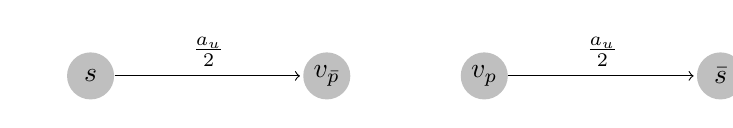
\begin{tikzpicture}[shorten >=1pt,->]
  \tikzstyle{vertex}=[circle,fill=black!25,minimum size=17pt,inner sep=0pt]

  \node[vertex] (G-s) at (0,0) {$s$};
  \node[vertex] (G-np) at (3,0) {$v_{\bar{p}}$};  
  \draw (G-s) -- (G-np) node[midway,above] {$\frac{a_u}{2}$};
    
  \node[vertex] (G-p) at (5,0) {$v_{p}$};    
  \node[vertex] (G-ns) at (8,0) {$\bar{s}$};      
  \draw (G-p) -- (G-ns) node[midway,above] {$\frac{a_u}{2}$};
  
\end{tikzpicture}
\end{center}

Similarly, pairwise terms with literals $p,q$ have edges $\edge{v_p}{v_{\bar{q}}} $ and $\edge{v_q}{v_{\bar{p}}}$. The full graph is given by
\begin{align*}
	\mathcal{V} =& \{ v_p \; | \; p \in L \} \cup \{s,\bar{s}\} \\[1em]
	\mathcal{E} =& \big\{ \edge{s}{v_{\bar{p}}},\edge{v_p}{t} \; | \; \forall a_p>0 \big\} \cup \big\{ \edge{v_p}{v_{\bar{q}}}, \edge{v_q}{v_{\bar{p}}} \; | \; \forall a_{pq} > 0 \big\}  \\[1em]
	c(\, (v_p,v_q)\, ) = c_{pq} =& \left\{ \begin{array}{rl}
		a_{p}/2, & \text{if } v_p \notin \{s,\bar{s}\} \text{ or } v_q \notin \{s,\bar{s}\} \\
		a_{pq}/2, & \text{if } v_p,v_q \notin \{s,\bar{s}\}\\ 
		0,& \text{otherwise}.
	\end{array}\right.
\end{align*}
%
A construction of graph $G_{\phi}$ is illustrated in~\cref{ch2:fig:posiform-capacitated-graph-a}. Therefore, the posiform $\phi$ can also be written as $\phi = \sum_{ \edge{v_p}{v_q} \in \mathcal{E}}{ c_{p\bar{q}} }$. In fact, it is possible to shown that there is a bijection between the posiform with zero constant $\phi$ and the graph $G_{\phi}$.


A flow is a function $\varphi:\mathcal{E}\rightarrow \mathbb{R}_{+}$ that satisfies
\begin{equation*}
	\begin{array}{rll}
	\displaystyle
	\varphi(\,\edge{v_p}{v_q}\,) = \varphi (p,q) <& c_{pq},&  \forall v_p,v_q \in \mathcal{V} \\[1em]
	\displaystyle
	\sum_{v_p \in \mathcal{V}}{\varphi(p,q)} =& \displaystyle \sum_{v_p \in \mathcal{V}}{\varphi (q,p)}, & \forall v_q \in \mathcal{V}.	
	\end{array}
\end{equation*}
%
A flow $\varphi ^{\star}$ is said to be maximum if 
\begin{align*}
	\varphi ^{\star} &= \argmax_{\varphi} \sum_{v_p \in \mathcal{V}}{\varphi(s,v_p)},
\end{align*}
%
i.e., if the flow leaving the source is maximum. The residual graph of $G_{\phi}$ with respect to some flow $\varphi$ is denoted $G_{ \phi [ \varphi ] }(\mathcal{V},\mathcal{E}^+,r)$ and owns the same set of vertices of $G_{\phi}$. The set of edges is extended to include returning edges as well, i.e.,
\begin{align*}
	\mathcal{E}^+ &= \mathcal{E} \cup \{ \edge{v_q}{v_p} \; | \; \edge{v_p}{v_q} \in \mathcal{E} \}.
\end{align*}
%
The edges cost is given by the residual function $r$
\begin{align*}
	r(\, \edge{v_p}{v_q} \, ) = r_{pq} &= \left\{ \begin{array}{ll}
	c_{pq} - \varphi( p,q ), & \edge{v_p}{v_q} \in \mathcal{E}\\
	\varphi( p,q ), & \edge{v_p}{v_q} \in \mathcal{E}^+ \setminus \mathcal{E}.
\end{array}\right.	 
\end{align*}
%
One can also construct a posiform from the residual graph $G_{ \phi [ \varphi ] }$. In this case, the posiform is denoted $\phi_{G_{ \phi [ \varphi ] }}$. We remark that edges arriving in the source or leaving the target are all mapped to $0$, as the source and the target are identified with the constants $1,0$ respectively. For example, $\edge{p}{s}$ is encoded as $p\bar{s}=0$.

The \emph{Ford-Fulkerson} algorithm computes the maximum flow by incrementing an initial zero flow function $\varphi_0=0$ every time an \emph{augmenting path} is found. The $k$-th augmenting path is a path $\pi_k = (p_0=s,p_1,p_2,\cdots,p_n,p_{n+1}=\bar{s})$ in the residual graph $G_{ \phi [\varphi_{k-1}] }$ in which all edges of $\pi_k$ have a positive residual value. We say that $\pi_k$ is an $\epsilon$-augmenting path if 
\begin{align*}
	\epsilon = \min_{p_i \in \pi_k\setminus {\bar{s}}} r_{p_i,p_{i+1}}.
\end{align*}
%
\begin{figure}
\center
\subfloat[Initial graph $G_{\phi}$ for $\phi = 2x + 8z + 2x\bar{z} + 4\bar{x}y + 6\bar{y}\bar{z}$\label{ch2:fig:posiform-capacitated-graph-a}]{
\includegraphics[scale=0.1]{figures/chapter2/master-posiform/posiform-graph-1.png}
}\\
\subfloat[$1$-Augmenting path $1$]{
\includegraphics[scale=0.1]{figures/chapter2/master-posiform/posiform-graph-2.png}
}%
\subfloat[$1$-Augmenting path $2$]{
\includegraphics[scale=0.1]{figures/chapter2/master-posiform/posiform-graph-3.png}
}\\%
\subfloat[$1$-Augmenting path $3$]{
\includegraphics[scale=0.1]{figures/chapter2/master-posiform/posiform-graph-4.png}
}%
\subfloat[$1$-Augmenting path $4$]{
\includegraphics[scale=0.1]{figures/chapter2/master-posiform/posiform-graph-5.png}
}\\%
\subfloat[Final residual graph $G_{ \phi {[\varphi^{\star}]} }$. The master posiform is written as $ { \phi^{\star} } = 4 + 2z +2\bar{z}\bar{y} + 4zy + 4\bar{y}x + 2z\bar{x}$]{
\includegraphics[scale=0.1]{figures/chapter2/master-posiform/posiform-graph-6.png}
}%
\caption{\textbf{Example of max-flow to find the master posiform}. The Ford Fulkerson algorithm is executed for the capacitated graph representation of posiform $\phi$. In~(a), the initial capacitated graph; a sequence of augmenting paths (we omit the returning edges) are shown in figures~(b-e); the final residual graph is shown in figure~(f).  }
\label{ch2:fig:posiform-capacitated-graph}
\end{figure}
%
\begin{proposition}{Residual graph to posiform}
	Given a posiform 
	\begin{align*}
		\phi = C(\phi) + \sum_{p \in L}{a_pp} + \sum_{p,q \in L}{a_{pq}pq},
	\end{align*}
	
	construct its corresponding capacitated graph $G_{\phi}$ and compute its maximum flow executing the Ford Fulkerson algorithm. Then, for every step $k$ of the algorithm we have that
	\begin{align*}
		\phi &= C(\phi) + \nu(\varphi_k) + \phi_{ G_{ \phi [\varphi_k]}}.
	\end{align*}
\end{proposition}
%
\begin{proof}

We observe that every $\epsilon$-augmenting path $\pi_k = s,v_{p_1},v_{p_2},\cdots,v_{p_n},\bar{s}$ in $G_{\phi [\varphi_k]}$ encodes an alternating sum of literals of the form
\begin{align*}
	\phi_{\pi_k} =& a_1\bar{p}_1 + a_{1\bar{2}}p_1\bar{p}_2 + a_{2\bar{3}}p_2\bar{p}_3 + \cdots + a_{n-1\bar{n}}p_{n-1}\bar{p}_k + a_np_n \\
	=&\epsilon( \bar{p}_1 + p_1\bar{p}_2 + p_2\bar{p}_3 + \cdots + p_{n-1}\bar{p}_n + p_n ) + \phi ',
\end{align*}
%
where
\begin{align*}
	\phi ' &= (a_{\bar{1}}-\epsilon)\bar{p}_1 + (a_{1\bar{2}} - \epsilon) p_1\bar{p}_2 + (a_{2\bar{3}}  - \epsilon)p_2\bar{p}_3 + \cdots + (a_{n-1\bar{n}} - \epsilon)p_{n-1}\bar{p}_n + (a_n -\epsilon)p_n.
\end{align*}
%
By observing that
\begin{align*}
	\bar{p}_1 + p_1\bar{p}_2 &= 1 - p_1p_2 \\
	-\bar{p}_{j-1}p_{j} + p_j\bar{p}_{j+1} &= \bar{p}_{j-1}p_j - p_jp_{j+1} \\
	-p_{n-1}p_n + p_n &= \bar{p}_{n-1}p_n,
\end{align*}
%
we can rewrite the alternating sum as
\begin{align*}
	\phi_{\pi} &= \epsilon + \epsilon( \bar{p}_1p_2 + \bar{p}_2p_3 + \cdots + \bar{p}_{n-1}p_n ) + \phi ' \\
	&= \psi + \phi ',	
\end{align*}
%
Note that $\phi '$ and $\psi$ corresponds, respectively, to the update of the residual costs for the edges of $\pi_k$ and the updates of its returning edges. Therefore, we can write
\begin{align*}
	\phi &= C(\phi) + \nu(\varphi_k) + \phi_{ G_{ \phi [\varphi_k] }},
\end{align*}
%
i.e., the initial posiform $\phi$ can be rewritten as a constant plus the posiform corresponding to the residual graph at step $k$ of  the Ford Fulkerson algorithm. 
\end{proof}
%
It follows that the master posiform is given by
\begin{align*}
	\phi^{\star} &= C(\phi) + \nu(\varphi^{\star}) + \phi_{ G_{ \phi [ \varphi^{\star}] }}.
\end{align*}
%
\begin{example}
The posiform $\phi = 2x + 8z + 2x\bar{z} + 4\bar{x}y + 6\bar{y}\bar{z}$ is represented by the graph $G_{\phi}$ in~\cref{ch2:fig:posiform-capacitated-graph}. Its maximum flow value  equals to $4$ and the master posiform is given by $\phi^{\star} = \nu(\varphi ^{\star}) + \phi_{G_{\phi {[\varphi^{\star}}]}} = 4 + 2z + 2\bar{z}\bar{y} + 4zy + 4\bar{y}x + 2z\bar{x}$.
\end{example}
%
From the strong persistency theorem we conclude that $z=0$, and we have
\begin{align*}
	\min \phi = \min \phi^{\star}(z=0) = \min 2\bar{y} + 4\bar{y}x.
\end{align*}
%
We can say more. Let $U$ be the set of literals that are reached from the source by a path of positive residual in the final residual graph. Then, a solution $\vec x \in \argmin f$ must agree with $x(U=1)$~\cite{boros02pseudo}. Therefore,
\begin{align*}
	\min \phi = \min \phi^{\star}(\bar{z}=1,y=1) = \min 4 = 4.
\end{align*}
%
In fact, by looking at all configurations of $\phi$, we observe that $(z=0,y=1)$ in every minimum configuration of $f$.

\begin{center}
\begin{tabular}{|c|c|c|c|}
\hline
$x$ & $y$ & $z$ & $f$\\
\hline
0 & 0 & 0 & 6 \\
0 & 0 & 1 & 8 \\
\textbf{0} & \textbf{1} & \textbf{0} & \textbf{4} \\
0 & 1 & 1 & 12 \\
1 & 0 & 0 & 10 \\
1 & 0 & 1 & 10 \\
\textbf{1} & \textbf{1} & \textbf{0} & \textbf{4} \\
1 & 1 & 1 & 10 \\
\hline
\end{tabular}
\end{center}

The construction above is the core of the \emph{QPBO} algorithm~\cite{boros91} that finds partial solutions of general quadratic PBF. \daniel{The labeled variables by QPBO are guarantee to belong to an optimum solution. This last property is usually referred as the \emph{partial optimality property} of QPBO, and it is a consequence of the strong persistency theorem.} In the most cases, the master posiform allows us to eliminate only few variables, but if the function $f$ is a \emph{submodular} function, QPBO finds the minimum of $f$.

%The master posiform $\phi^{\star}(f)$ gives us a lower bound for the PBF $f$, which is called the roof dual. In some fortunate occasions, the master posiform allows us to simplify the original optimization problem in a trivial one. That is the case for the class of \emph{submodular} functions.


\subsection{Submodularity}

\begin{definition}{Submodular set function}

Let $V$ be a set with $n$ elements, e.g., $V=\{1,2,\cdots, n\}$. A set function $f:2^V\rightarrow \mathbb{R}$ is submodular if 
\begin{align}
	f(X) + f(Y) \geq f(X \cup Y) + f(X \cap Y),\quad \forall X,Y \subset V.
	\label{ch2:eq:submodular-set-function}
\end{align}
%
\end{definition}
%
An equivalent local definition is given by
\begin{align}
	f(X \cup \{x_1\}) + f(X \cup \{x_2\}) \geq f(X \cup \{x_1,x_2\}) + f(X), \; \forall X \subset V \text{ and } \{x_1,x_2\} \not\subset X.
	\label{ch2:eq:submodular-local}
\end{align}
%
\begin{proposition}{Quadratic submodular PBF}
	Let $f:2^V\rightarrow \mathbb{R}$ a quadratic PBF  written as
	\begin{align*}
		f(x_1,\cdots,x_n) &= C + \sum_{i<n}{f_{i}(x_i)} + \sum_{i<j<n}{f_{ij}(x_i,x_j)}.
	\end{align*}
	Then, the statements below are equivalent
	\begin{itemize}
	 	\item[i]{Function $f$ is submodular.}
		\item[ii]{ $f_{ij}(0,1) + f_{ij}(1,0) \geq f_{ij}(0,0) + f_{ij}(1,1), \quad \forall i<j<n$}
		\item[iii]{ $\frac{\partial^2 f}{\partial x_i\partial x_j} \leq 0, \quad \forall i<j<n$ }
	\end{itemize}
\end{proposition}	
%
	\begin{proof}
	
	\begin{tabular}{rl}
	$\mathbf{(i\rightarrow ii)}$:& Immediately from~\cref{ch2:eq:submodular-local}. \\	
	$\mathbf{(ii\rightarrow iii)}$:&  Writing down the terms in $f$ for variables $x_i,x_j$ we have
	\end{tabular}
	\begin{align*}
		f_{ij}(0,0)(1-x_i)(1-x_j) + f_{ij}(1,1)x_ix_j + f_{ij}(0,1)(1-x_i)x_j + f_{ij}(1,0)x_i(1-x_j).
	\end{align*}
%
	Taking its second derivative
	\begin{align*}
		\frac{\partial^2f}{\partial x_i\partial x_j} &= f_{ij}(0,0) + f_{ij}(1,1) - f_{ij}(0,1) - f_{ij}(1,0) \leq 0.
	\end{align*}
%	
	\begin{tabular}{rl}
		$\mathbf{(iii\rightarrow i)}$:& We define
	\end{tabular}		
		\begin{align*}
			\Delta_{x_i} &= f(x_1,\cdots,x_{i-1},x_i=1,x_{i+1},\cdots,x_n) - f(x_1,\cdots,x_{i-1},x_i=0,x_{i+1},\cdots,x_n) \\
			&= f(X \cup \{x_i\}) - f(X), \quad \text{ where } x_i \notin X.
		\end{align*}		 		
		Therefore
		\begin{align*}
			f( X \cup \{x_1,x_2\}) &= f(X) + \Delta_{x_1} + \Delta_{x_2} + \frac{ \partial^2 f}{\partial x_i \partial x_j} \\
			f( X \cup \{x_1,x_2\}) &= -f(X) + f(X \cup \{x_1\}) + f(X \cup \{x_2\}) + \frac{ \partial^2 f}{\partial x_i \partial x_j}.
		\end{align*}	
%		
		Finally,
		\begin{align*}
			f( X \cup \{x_1,x_2\}) +f(X) - f(X \cup \{x_1\}) - f(X \cup \{x_2\}) &\leq 0.	
		\end{align*}
%		
	\end{proof}

Supermodular functions, on the other hand, are functions that satisfy
\begin{align*}
	f(X) + f(Y) \leq f(X \cup Y) + f(X \cap Y),\quad \forall X,Y \subset V.
\end{align*}
%
Therefore, if $f$ is submodular, $-f$ is supermodular. \daniel{The QPBO algorithm efficiently computes the minimum (maximum) of submodular (supermodular) functions. The opposite problem, i.e., maximizing (minimizing) a submodular (supermodular) function is in $NP$-hard. }

There are functions which are \daniel{neither} submodular \daniel{nor} supermodular and are called \emph{non-submodular}. Optimizing a non-submodular function is in $NP$-hard but QPBO can be used to find a \daniel{partially optimal solution}, as noticed previously.  \daniel{Nonetheless, it is likely the case that QPBO will leave several variables unlabeled while minimizing a non-submodular energy. To attenuate this problem, two variations of QPBO were proposed in~\cite{rother07qpbo}}
\daniel{
\begin{itemize}
	\item[]{\textbf{QPBO-Probe}: Implements a branch-and-bound technique in an attempt to increase the number of variables labeled by QPBO. It keeps the partial optimality property.}
	\item[]{\textbf{QPBO-Improve}: An heuristic that is guaranteed to return a labeling of lower or equal value than the labeling giving by QPBO. The partial optimality property is lost.}
\end{itemize}}
As discussed in~\cref{ch2:sec:markov-random-fields,ch2:sec:pseudo-boolean-functions}, several problems in image processing can be modeled in terms of an HMM $\mathcal{H}$ defined over the image grid graph. The hidden states of $\mathcal{H}$ are often estimated as the maximum likelihood of the induced probability distribution given the set of observed variables $\vec{Y}$. \daniel{In that occasion, we mention that the success of this approach depended on the difficulty of the maximum likelihood computation. We observed that the general problem is in NP-Hard for multilabel HMM, and we turn our attention to binary ones. In this case, we have to solve a PBF optimization problem.}

As we have seen, the optimization of a PBF is closely related with the computation of maximum flows, or equivalently, minimum cuts in a graph.\daniel{ In fact, in some applications such as binary segmentation, it is more practical to think in terms of a minimum cut problem than in terms of an HMM one. Both interpretations are equivalent and trigger different insights, but the graph cut mindset fits very nicely in the binary segmentation framework and it gives to us an implicit representation of a digital contour, which can be exploited to incorporate geometric information in the model.} %and  The last interpretation is quite convenient in some applications such as binary segmentation. In fact, to think of the problem as we are going to see in the next section that is more practical to think on the problem as a minimum-cut The cut The HMM machinery can be  as the  a point of view is quite enlightening, as we can interpret problems in imaging with the computation of minimum cuts in its grid graph. In the next chapter we \daniel{describe two models inspired in this idea.}


\section{Graph cut models}
\label{ch2:sec:graph-cut-models}

\daniel{ Graph cut techniques in imaging were pioneered by~\cite{greig89exact} and became popular after the interactive binary segmentation model proposed by~\cite{boykov01graphcut}. In this section, we are going to describe the latter and two other applications of graph cut techniques. The first explains how to set the cost function to estimate perimeter of segmented shapes and the second one extends the first by incorporating a constraint that helps in the segmentation of thin and elongated objects.}

\subsection{Binary segmentation}

Let $\vec{I} \in \mathbb{F}^{m\times n}$ a discrete grayscale image and $\GG (\mathcal{V},\mathcal{E})$ its grid graph. We denote $\vec{x}$ the vector of binary variables indexed by image pixels, i.e., $x_p$ is associated to pixel $p$. We consider the capacitated grid graph $\GGe (\mathcal{V}^+,\mathcal{E}^+,c)$ where 
%It is a binary labeling problem. We present here its formulation as an HMM.
\begin{align*}
	\mathcal{V}^+ &= \mathcal{V} \cup \{s,t\} \\
	\mathcal{E}^+ &= \mathcal{E} \cup \big\{ \{s,v_p\}, \{v_p,t\} \; | \; p \in \vec{I} \big\}.
\end{align*}
The cost function $c$ is defined later. The members of the additional set of edges are referred to as terminal edges. Next, let sets $\mathcal{V}_{fg}, \mathcal{V}_{bg} \subset \mathcal{V}$ to represent foreground and background seeds furnished by the user. A $(s,t)$-cut set of $\GGe$ partitions the graph in connected components $S,T$. The first connected to the source and the other to the target vertex. Vertices in $\mathcal{V}_{fg}$ ($\mathcal{V}_{bg}$) will be forced to be in the source (target) component after the removal of a $(s,t)$-cut set.

The data term is modeled by
\begin{align*}
	\psi_1(x_p) &= \left\{ \begin{array}{ll}
	-\ln  H_{bg}\big( I(p) \big), & \text{if } x_p=0  \\[1em]	
	-\ln  H_{fg}\big( I(p) \big), & \text{if } x_p=1,
	\end{array}\right.
\end{align*}
where $H_{bg},H_{fg}$ are mixed Gaussian distributions derived from foreground and background seeds. We associate the $0$ value to the background label and the $1$ value to the foreground label. The space coherence term is expressed as
\begin{align*}
	\psi_{2}(x_p,x_q) &= \left\{ \begin{array}{ll}
	\displaystyle \exp{ \left(- \frac{1}{d_E(p,q)}\frac{(I(p) - I(q))^2}{2\sigma^2} \right) }, & q \in \mathcal{N}_k(p) \\[1em]
	0, & \text{otherwise},
	\end{array}\right.
\end{align*}
%
where $d_E(p,q)$ is the Euclidean distance between the pixel coordinates of $p,q$ and $\lambda$ is the parameter to control the influence of the terms in the energy. The value $\sigma$ is interpreted as a parameter to configure noise level of the input image; and $k$ denotes the chosen neighborhood cardinality of the graph (e.g. $8$).

Finally, given weights $\gamma_r \geq 0$ and $\gamma_b \geq 0$, we define the cost function $c:\mathcal{E}^+\rightarrow \mathbb{R}$ as

\begin{table}[h]
\center
\setlength{\extrarowheight}{0.75em}
\begin{tabular}{|c|c|l|}	
\hline
	\multicolumn{1}{|c|}{\textbf{edge} $\mathbf{e}$} & \multicolumn{1}{c|}{$\mathbf{c(e)}$} & \multicolumn{1}{c|}{\textbf{for}}\\
	\hline
	$\{v_p,v_q\}$ & $\gamma_b \cdot \psi_{2}(x_p,x_q)$ & $\forall p \in \vec{I} \text{ and } q \in \mathcal{N}_k(p)$\\
	\hline
	\multirow{3}{*}{ $\{v_p,s\}$ } & $\gamma_r \cdot \psi_1(x_p=0)$ & $\forall p \in \vec{I} \text{ and } p \notin \mathcal{V}_{fg} \cup \mathcal{V}_{bg}$\\
	& $M$ & $p \in \mathcal{V}_{fg}$ \\
	& $0$ & $p \in \mathcal{V}_{bg}$\\
	\hline
	\multirow{3}{*}{ $\{v_p,t\}$ } & $\gamma_r \cdot \psi_1(x_p=1)$ & $\forall p \in \vec{I} \text{ and } p \notin \mathcal{V}_{fg} \cup \mathcal{V}_{bg}$\\
	& $0$ & $p \in \mathcal{V}_{fg}$ \\
	& $M$ & $p \in \mathcal{V}_{bg}$. \\
	\hline
\end{tabular}
\begin{align*}
\text{where,} \qquad M = 1 + \max_{p \in \vec{I}}{\gamma_b \sum_{q \in \mathcal{N}_k(p)}}{\psi_2(x_p,x_q)}.
\end{align*}
\end{table}

Notice that each vertex in $\mathcal{V}$ must have one and only one of its terminal edges in a cut set. Let $\mathcal{E}'$ be a cut set partitioning $G_{I+}$ in connected components $(S,T)$, the first connected to the source and the other connected to target. Its cut value is written as 
\begin{align}
	E^{gcut}(\GGe,\mathcal{E}') &= \gamma_r \left( \sum_{v_p \in S}{ \psi_1(1) } +\sum_{v_p \in T}{\psi_1(0)} \right) + \gamma_b \sum_{(v_p,v_q) \in \mathcal{E}'}{\psi_2(0,1)}.
\label{ch2:eq:graphcut-cut-value}
\end{align}
%
We observe that~\cref{ch2:eq:graphcut-cut-value} can also be written in the form of the Gibbs energy
\begin{align}
	\gamma_r \sum_{x_p \in \vec{X}}{ \psi_1(x_p) } + \frac{\gamma_b}{2}\sum_{ \substack{x_p,x_q \in \vec{X} \\ x_p \neq x_q }}{\psi_2(x_p,x_q)}.
	\label{ch2:eq:graph-cut-gibbs}
\end{align}
%
%
Therefore, a minimum $(s,t)$-cut of $\GGe$ induces a labeling of minimum value for~\cref{ch2:eq:graph-cut-gibbs}. Vertices connected to the source component of the cut are labeled as foreground and those connected to the target are labeled as background. This interpretation is quite natural for the binary segmentation problem, as a minimum $(s,t)$-cut of the grid graph gives a binary partition of the image. In this sense, one could abstract the HMM machinery underneath and simply construct a graph such that its minimum cut separates the desired objects.

\begin{figure}
\center
\subfloat{
\includegraphics[scale=0.25]{figures/chapter2/grabcut/coala/seeds.png}
}
\subfloat{
\includegraphics[scale=0.25]{figures/chapter2/grabcut/coala/gc-seg.png}
}\hspace{1em}
\subfloat{
\includegraphics[scale=0.25]{figures/chapter2/grabcut/vase/seeds.png}
}
\subfloat{
\includegraphics[scale=0.25]{figures/chapter2/grabcut/vase/gc-seg.png}
}
\caption{\textbf{Graph cut segmentation}. Foreground seeds are colored in green and background seeds are colored in blue.}
\end{figure}

Given the particular topology of grid graphs, specific versions of max-flow algorithms were conceived for them. A scalable version of graph cut algorithm~\cite{delong08scalable} can be used for images of high resolution; if several flows should be computed for similar graphs (video sequence segmentation), one can use the flow recycling algorithms~\cite{kohli05efficiently,juan06active}. Although the general complexity of these alternatives may be higher than Ford-Fulkerson algorithm, they are reported~\cite{szeliski06comparative} to compute minimum cuts in lower time for grid graphs.

\subsection{Geodesics computation}

We have seen the natural connection between cuts and binary segmentation describing the graph cut algorithm. The removal of a cut $\mathcal{E}'$ set partitions the grid graph in two disjoint connected components, one connected to the source and associated to the foreground and the other connected to the target and associated to the background. The cut $\mathcal{E}'$ itself can be related with the contour $\partial S$ of the foreground shape (see~\cref{ch2:fig:geodesic-grid-graph-shape-intersection}). In~\cite{boykov03geodesics} it was shown that one can define a cost function for the edge set $\mathcal{E}$ such that the cost of $\mathcal{E}'$ is arbitrarily close to the length of $\partial S$.

The key idea is to use the Cauchy-Crofton formula from integral geometry. In $2D$, let $\mathcal{L}$ be the set of all straight lines in the plane and $d\mathcal{L}$ a Lebesgue measure on this set. Then, the perimeter of a shape $S$ is given by
\begin{align*}
\int_{}{n_c}d{\mathcal{L}} = 2|\partial S|,
\end{align*}
%
where $n_c$ is the number of intersections of some line in $\mathcal{L}$ with the shape contour. To compute the Euclidean length, the cost function should be set as
\begin{align*}
	w_k &= \frac{ \delta^2 \Delta \phi_k }{2 |e_k|},
\end{align*}
%
where $\delta$ is the distance between two lines in the same family and $\Delta \phi_k$ is the angle difference between two consecutive lines (counterclockwise orientation) of different directions in the neighborhood system (see~\cref{ch2:fig:geodesic-grid-graph-shape-intersection}).

\begin{figure}
\center
\includegraphics[scale=0.5]{figures/chapter2/perimeter-graph-cuts/geodesics.eps}
\caption{\textbf{Computing perimeter via graph cuts}. The perimeter of a shape $S$ can be encoded as the value of some cut in the grid graph. In the figure, the contour of shape $S$ intersects a set $C \in \mathcal{E}$ of the grid graph with neighborhood system $\mathcal{N}_8$. One can set a cost function on $\mathcal{E}$ such that the cost of $C$ converges to the length of $\partial S$ as the neighborhood system goes to infinity.}
\label{ch2:fig:geodesic-grid-graph-shape-intersection}
\end{figure}

The authors proved equivalent results for an arbitrary Riemannian metric in two and three dimensions. A drawback of this approach is that the quality of the results are very sensitive to the neighborhood system. Small neighborhoods are prone to metrication errors and the convergence theorem, although of theoretical importance, it does not possess the \emph{multigrid convergence} property. The $4$-neighborhood system returns a poor estimation of length no matter the image resolution. We discuss multigrid convergence in~\cref{chapter:digital-geometry}.

Another interesting contribution in the attempt to inject geometric information in the graph cut framework is the connectivity priors of~\cite{vicente08graph}. This work provides an additional tool to the graph cut algorithm in which the user select points of the image that should be connected to the foreground component. An heuristic based on the Dijkstra algorithm for shortest paths is computed using a metric based on the color intensities. The method proved very useful to the segmentation of thin and elongated objects (see~\cref{ch2:fig:graphcut-connectivity}).

\begin{figure}
\center
\subfloat[]{
\includegraphics[scale=0.15]{figures/chapter2/grabcut-connectivity/cp-1.png}
}
\subfloat[]{
\includegraphics[scale=0.15]{figures/chapter2/grabcut-connectivity/cp-2.png}
}
\subfloat[]{
\includegraphics[scale=0.15]{figures/chapter2/grabcut-connectivity/cp-3.png}
}
\subfloat[]{
\includegraphics[scale=0.15]{figures/chapter2/grabcut-connectivity/cp-4.png}
}
\caption{\textbf{Graph cut with connectivity priors}~\cite{vicente08graph}. In (a) the foreground (green) and background (blue) seeds. In (b) the graph cut segmentation. In (c) the points selected by the user in which the connectivity constraint is going to be applied. In (d) the final segmentation. }
\label{ch2:fig:graphcut-connectivity}
\end{figure}


%\subsubsection{Approximating multilabel energies with $\alpha$-expansion and $(\alpha,\beta)$-swap}
%
%For pseudo-boolean functions (binary labels), we know that the submodular class is minimized in polynomial time. For energies of order at most three, the problem is reduced to the computation of a minimum cut in a capacitated graph. For higher orders, the best algorithm has complexity $O(n^5Q + n^6)$~\cite{orlin09faster}, where $Q$ is the time to evaluate the function being minimized. If the function is not binary (multilabeling problems), things get more complicated.
%
%At first glance, the multilabeling extension does not seem to be an issue, as we can always transform a multilabel problem in a binary one by including as many as $\log |\Gamma_{\vec{X}}|$ new variables. The difficulty is that the resulting energy is likely  non-submodular~\cite{ramalingam08}, and the minimization of a general non-submodular function is in $NP$-hard. In this section we describe two algorithms to approximate the MAP inference of multilabel problems based on local-search.
%
%A standard approach to devise an approximation solution is the so called \emph{local-search} paradigm described in~\cref{ch2:alg:local-search-paradigm}. The local-search paradigm finds a local minimum (maximum) with respect to some given neighborhood $\mathcal{N}$ and an initial solution $x_0$. The difference between the global and optimum solutions is denoted the \emph{optimality gap}. Naturally, a larger neighborhood tends to decrease the optimality gap and may lead to an increase in the running time. In the extreme case, in which all configurations are present in the neighborhood $\mathcal{N}$, the local-search returns the global optimum solution. Therefore, a successful local-search algorithm is the one that has a good compromise between neighborhood size and optimality gap.
%
%\begin{algorithm}
% \LinesNumbered
% \SetKwInOut{Input}{input}\SetKwInOut{Output}{output}
% \SetKwRepeat{Do}{do}{while}%
% \SetKwComment{comment}{//}{}
% 
%  \Input{Function $f$; an initial solution $x^{(0)}$; and a neighborhood $\mathcal{N}$.}
%  \Output{Local minimum solution of $f$ with respect to neighborhood $\mathcal{N}$ and initial solution $x^{(0)}$.}  
%  \BlankLine
%  
% $t \longleftarrow 0$\;
% \Do{$f(x^{(t)}) < f(x^{(t-1)})$}{
% 	$x^{(t+1)} = \displaystyle \argmin_{ x \in \mathcal{N}(x^{(t)})} f(x)$ \tcp*[l]{Local optimization step} \nllabel{ch2:alg:local-search-local-opt-step} 
%	$t \longleftarrow t + 1$\; 	
% }
% \BlankLine
% 
% \caption{Local search paradigm for minimization.}
% \label{ch2:alg:local-search-paradigm}
%\end{algorithm}
%
%Approximation algorithms like iterated conditional moves (ICM)~\cite{besag86} and simulated annealing~\cite{geman84} defines the neighborhood $\mathcal{N}(\vec{I}^{(t)})$ as the set of images that differs in a single pixel from $\mathcal{N}(\vec{I}^{(t)})$. Consequently, a premature stop in a local optimum of lower quality is likely to happen. 
%
%The idea in the \emph{$\alpha$-expansion} and \emph{$(\alpha,\beta)$-swap} algorithms consists in to define a large neighborhood $\mathcal{N}(\vec{I}^{(t)})$ such that finding the best configuration in such neighborhood can be efficiently computed. In order to illustrate some ideas, let's consider once again the Potts model applied to image denoising of a grayscale image $\vec{I} \in \mathbb{F}^{m \times n}$.
%\begin{align}
%	\phi_{pq}(x_p,x_q) &= \left\{ \begin{array}{ll}
%		K,& \text{if } x_p \neq x_q \\
%		0,& \text{otherwise}.
%	\end{array}\right. \label{ch2:eq:potts-model-denoising-bis-1} \\[1em]
%	E(\vec{x}) &= \sum_{p \in \mathcal{V} }{\phi_p(x_p)} + \sum_{(p,q) \in \mathcal{E}}{\phi_{pq}(x_p,x_q)}.	
%	\label{ch2:eq:potts-model-denoising-bis-2}
%\end{align}
%%
%%
%As mentioned before, minimizing~\cref{ch2:eq:potts-model-denoising-bis-1,ch2:eq:potts-model-denoising-bis-2} is in NP-hard as long as variables $x_p,x_q$ take values in a set of cardinality greater than $2$. Notice that if we limit the problem to only two labels, let's say $\alpha,\beta$,~\cref{ch2:eq:potts-model-denoising-bis-1,ch2:eq:potts-model-denoising-bis-2} is a submodular PBF (Ising model) and can be minimized in polynomial time. The key is in to define the transformation function 
%\begin{align*}
%	T_{\alpha,\beta}(x_p,c_p) &= \left\{ \begin{array}{rl}
%		\alpha,& \quad \text{if } ( x_p=\alpha \text{ or } x_p=\beta) ) \text{ and } c_p=0,\\[1em]
%		\beta,& \quad \text{if } ( x_p=\alpha \text{ or } x_p=\beta) ) \text{ and } c_p=1,\\[1em]
%		x_p,& \quad \text{otherwise}.
%	\end{array}\right. ,
%\end{align*}
%%
%and the neighborhood
%\begin{align*}
%\mathcal{N}_{\alpha,\beta}(\vec{I}) &= \left\{ \vec{I}' \; | \; \vec{I}'(p) = T_{\alpha,\beta}(\vec{I}(p),\{0,1\}) \quad \forall p \in \vec{I} \right\}.
%\end{align*}
%%
%%
%In the $(\alpha,\beta)$-swap algorithm, the local-optimization step (~\cref{ch2:alg:local-search-local-opt-step} in~\cref{ch2:alg:local-search-paradigm}) is replaced by
%
%\begin{algorithm}[H]
%  \BlankLine
%  
% 	\For{ $(\alpha,\beta) \in \{0,255\}$ }
% 	{
%	 	$y \longleftarrow \displaystyle \argmin_{ y' \in \mathcal{N}_{\alpha,\beta}(x^{(t)})} f(y')$\;
%	 	\If{ $f(y) < f(x^{(t)})$ }
%	 	{
%	 		$x^{(t)} \longleftarrow y$\;
%	 	}
% 	}
% 	
% \BlankLine
%\end{algorithm}
%
%\begin{figure}
%\center
%\subfloat[Original image]{
%\includegraphics[scale=0.1]{figures/chapter2/move-making/move-making-1.png}
%}%
%\subfloat[Noisy image]{
%\includegraphics[scale=0.1]{figures/chapter2/move-making/move-making-2.png}
%}%
%\subfloat[$\alpha$-expansion]{
%\includegraphics[scale=0.1]{figures/chapter2/move-making/move-making-3.png}
%}%
%\subfloat[Range moves]{
%\includegraphics[scale=0.1]{figures/chapter2/move-making/move-making-4.png}
%}
%\caption{\textbf{$\mathbf{\alpha}$-expansion x range moves}\cite{veksler07graph}.Comparison of $\alpha$-expansion $\big( (\alpha,\beta)$-swap results are similar$\big)$ and range moves for denoising a piecewise smooth image using the truncated convex potential $\phi_2(x_p,x_q) = \min \{ (x_p-x_q)^2,50 \}$. The range move algorithm returns a smoother image than $\alpha$-expansion. }
%\label{ch2:fig:move-making-examples}
%\end{figure}
%
%The $\alpha$-expansion works in a similar way, except that the only movement allowed is to change a label to some other label $\alpha$. In the $(\alpha,\beta)$-swap algorithm the local optimization energy is submodular if
%\begin{align}
%	\phi_{pq}(\alpha,\alpha) + \phi_{pq}(\beta,\beta) \leq \phi_{pq}(\alpha,\beta) + \phi_{pq}(\beta,\alpha) & \quad \forall \alpha,\beta \in \Gamma_{\vec{X}}.
%	\label{ch2:eq:multilabeling-metric}
%\end{align}
%%
%In the case of $\alpha$-expansion, submodularity is ensured if
%\begin{align}
%	\phi_{pq}(\alpha,\alpha) + \phi_{pq}(\beta,\gamma) \leq \phi_{pq}(\beta,\alpha) + \phi_{pq}(\alpha,\gamma) & \quad \forall \alpha,\beta,\gamma \in \Gamma_{\vec{X}}.
%	\label{ch2:eq:multilabeling-semi-metric}	
%\end{align}
%%
%The $\alpha$-expansion and $(\alpha,\beta)$-swap algorithms have good overall performance for models based in the Potts potential. In~\cite{boykov01fast} we can find nice results for stereo. However, they are less appealing if we use a truncated convex $2$-clique potential~\cite{blake11markov}(see chapter 11). In this case, the \emph{range moves} algorithm proposed in~\cite{veksler07graph} is reported to deliver better results.



%Energies $\phi_{pq}$ that are metrics satisfy~\cref{ch2:eq:multilabeling-metric,ch2:eq:multilabeling-semimetric} and energies that are semi-metrics satisfy~\cref{ch2:eq:multilabeling-semi-metric} only. We recall that $\phi_{pq}$ is metric if
%
%
%\begin{align*}
%	\phi_{pq}(\alpha,\beta) \geq 0 & \quad \text{(Non-negative)} \\
%	\phi_{pq}(\alpha,\beta) = 0 \Leftrightarrow \alpha=\beta & \quad \text{(Null value implication)}\\
%	\phi_{pq}(\alpha,\beta) = \phi_{pq}(\alpha,\beta)  & \quad \text{(Symmetric)} \\
%	\phi_{pq}(\alpha,\beta) \leq \phi_{pq}(\alpha,\gamma) + \phi_{pq}(\gamma,\beta)  & \quad \text{(Triangle inequality)}.
%\end{align*}
%
%A semi-metric is any function that satisfy all conditions above, except the triangle inequality. Examples of metric and semi-metric functions
%
%\begin{align*}
%	f(x,y) &= \min{ \big( K,(I(x)-I(y))^2 \big)} \quad \text{semi-metric} \\
%	f(x,y) &= \min{ \big( K,|I(x)-I(y)| \big) } \quad \text{metric} \\ 
%	f(x,y) &= \left\{ \begin{array}{rl}
%		K,& \text{if } x \neq y \\
%		0,& \text{otherwise}.
%	\end{array}\right.  \quad \text{metric}
%\end{align*}


%\section{GraphCut}
%\subsection{Submodular to graph-cut}
%\subsection{Grabcut}
%\subsection{alpha expansion, alfa-beta swap}
%\section{Image denoising}
%\section{Image segmentation}
%	\subsection{Graph-cuts}
%	\subsection{Watersheds}
%	\subsection{Morphology}	
%	\subsection{Thresholding}		
%	\subsection{Wavelets}		
%	\subsection{Corner, edge detection, filters}
%	\subsection{Region adjacenty graph}
%	\subsection{K-means segmentation}	
%	\subsection{Hough transform, parameter space}
%\section{Image inpainting}	

%	\chapter{Curvature Prior}
\label{chapter:curvature-prior}

\sketch{
\begin{enumerate}
	\item{Motivation}
	\begin{itemize}
		\item{Curvature properties}
	\end{itemize}
	\begin{itemize}
		\item{Constraint optimization models}
		\item{Combinatorial optimization models}		
		\item{Continuous models}
	\end{itemize}
	
\end{enumerate}
}
%	\chapter{Digital Geometry}
\label{chapter:digital-geometry}

The primitives of Euclidean geometry, such as lines and points, are idealized objects. A line segment is infinitely thin and a point is dimensionless. When referring to such entities, we eventually make use of visual representations and the line is incarnated as a trace and the point as a dot in the white board, for example. As long as we have the mathematical description of some shape $S$, we do not need any visual representation of it to compute its tangents, curvatures or perimeter. 

In imaging, however, it is almost always the case that we do not have a mathematical description of the objects in the scene. We need to identify the primitives from its visual representations.  We are not dealing with idealized objects anymore, but with finite descriptions of them. One of the subjects of study of digital geometry, and the one focused in this chapter, is how to correctly measure geometric properties in digitized objects.

We introduce basic concepts of digital geometry in~\cref{ch5:sec:ground-concepts} and we point out the difference between exact sampling and digitization. In~\cref{ch5:sec:geometric-measurements}, we introduce the multigrid convergence property and we give examples of several multigrid convergent estimators for local and global geometric measurements.

%As an illustration, consider the following examples of problems related with convex sets arising from each of this sub fields
%
%\begin{itemize}
%	\item[]{\textbf{Geometry}: What is the convex polygon of smallest area enclosing a shape $S$?}
%	\item[]{\textbf{Computational Geometry}: Given $n$ sample points of $S$, one can compute its convex hull in time $O(n \lg n)$.}
%	\item[]{\textbf{Discrete/Combinatorial geometry}: Take any $100$ convex sets in $R^2$ and denote them by $C_1, \cdots C_n$. If $C_i \cap C_j \cap C_k \neq \emptyset$, then $\bigcap C_i \neq \emptyset$.}
%	\item[]{\textbf{Digital geometry}: Let $D_h(S)$ be the digitization of a convex shape $S$. Can we devise a tangent estimator that is monotone with respect to some order in the digital boundary of $S$ for all its digitizations (different values of $h$)?}
%\end{itemize}


\section{Ground concepts}\label{ch5:sec:ground-concepts}

In this section we define the grid point model and its adjacency relations, which allow us to define the digital line primitive. Next, we describe the grid intersection and Gauss digitization mappings, which link continuous objects to its digital representations in the grid point model. The concepts defined in this section can be explored in much more depth in the book~\cite{klette04digital}.

\subsubsection{Digital grid, digitization and digital line}

\begin{definition}{$2D$ Digital grid}
The $2D$ digital grid $h\mathbb{Z}^2 = \{ p = (h \cdot i,h \cdot j) \; | \; i,j \in \mathbb{Z}\}$ with grid step (resolution) $h \in \mathbb{R}^+ \setminus \{0\}$ is a regular sampling of the plane. Its members are called \emph{grid points}.
\end{definition}

We can think of the digital grid as a regular tessellation of the plane. The grid points are the center of the \emph{grid squares} (pixels). The other components, \emph{grid edges } and \emph{grid vertices} are illustrated in~\cref{ch5:fig:grid-point-model}. They form the \emph{grid point model} of the plane. Next we define the two commonest adjacency relations in the grid point model.

\begin{figure}
\begin{minipage}{0.6\textwidth}
\center
\subfloat[Grid point model\label{ch5:fig:grid-point-model}]{
\includegraphics[scale=0.5]{figures/chapter-digital/digital-grid/grid-point-model.png}
}
\end{minipage}%
\begin{minipage}{0.4\textwidth}
\center
\subfloat[$4$-adjacency\label{ch5:fig:4-adjacency}]{
\includegraphics[scale=0.25]{figures/chapter-digital/digital-grid/4-adjacency.png}
}\hspace{1em}%
\subfloat[$8$-adjacency\label{ch5:fig:8-adjacency}]{
\includegraphics[scale=0.25]{figures/chapter-digital/digital-grid/8-adjacency.png}
}\\

\subfloat[Connected components\label{ch5:fig:connected-sets}]{
\includegraphics[scale=0.5]{figures/chapter-digital/digital-grid/connectivity.png}
}
\end{minipage}

\caption{\textbf{Digital grid and adjacency relations.} The grid point model and its components in (a); The $4$ and $8$ adjacency relations in (b) and (c); A $4$-connected set (orange) and a $8$-connected set (blue) in (d).}
\label{ch5:fig:digital-grid}
\end{figure}

\begin{definition}{$4$-adjacency relation}
Two grid points $p_1=(x_1,y_1)$ and $p_2=(x_2,y_2)$ are $4$-adjacent iff $p_1 \neq p_2$ and $|x_1-x_2| + |y_1-y_2| = 1$. We denote relation membership as $p_1A_4p_2$.
\end{definition}

\begin{definition}{$8$-adjacency relation}
Two grid points $p_1=(x_1,y_1)$ and $p_2=(x_2,y_2)$ are $8$-adjacent iff $p_1 \neq p_2$ and $\max \{ |x_1-x_2|, |y_1-y_2| \} = 1$. We denote relation membership as $p_1A_8p_2$.
\end{definition}

The adjacency relations are illustrated in~\cref{ch5:fig:4-adjacency,ch5:fig:8-adjacency}. Armed with an adjacency relation, we can define the notions of path and connectivity. A \emph{$4$-connected path} is a sequence $\{p_1,p_2,\cdots, p_n\}$ of grid points such that $p_iA_4p_{i+1}$ for all $1 \leq i < n$. A set $P$ is \emph{$4$-connected} if for every $p,q \in P$ there exists a $4$-connected path starting at $p$ and ending at $q$. Analogously definitions holds for $8$-adjacency relation~(see~\cref{ch5:fig:connected-sets}).


The adjacency relations are also used to define the $4,8$ neighborhood sets of a grid point.~
\begin{align*}
	\mathcal{N}_4(p) &= \{ q \; | \; pA_4q \}. \\
	\mathcal{N}_8(p) &= \{ q \; | \; pA_8q \}.
\end{align*}
Next, we are going to define mappings that will give us the grid point representation of  continuous objects.

\begin{definition}{Gauss digitization}
Let $S \subset \mathbb{R}^2$ a shape in the plane. Its Gauss digitization $D_h(S)$ in a digital grid of resolution $h \in \mathbb{R}^+\setminus \{0\}$ is defined as the set of grid points contained in $S$.
\end{definition}

\begin{figure}
\center
\subfloat[$h=1.0$]{
\includegraphics[scale=0.36]{figures/chapter-digital/digitization/h1.png}
}
\subfloat[$h=0.5$]{
\includegraphics[scale=0.18]{figures/chapter-digital/digitization/h05.png}
}
\subfloat[$h=0.25$]{
\includegraphics[scale=0.09]{figures/chapter-digital/digitization/h025.png}
}
\caption{\textbf{Gauss digitization.} Digitization of a ball of radius $5$ in three different resolutions.}
\label{ch5:fig:gauss-digitization}
\end{figure}

In~\cref{ch5:fig:gauss-digitization} we show the Gauss digitization of an Euclidean ball of radius $5$. As one could expect, the Gauss digitization is not adequate to the digitization of lines. In this case, the grid intersection digitization is preferred.

\begin{definition}{Grid intersection digitization}
The grid intersection digitization of a planar curve $\gamma$ is the set of all grid points in the digital grid that are closest (Euclidean distance) to the intersection points of $\gamma$ with the grid lines.
\end{definition}

\begin{figure}
\center
\subfloat[]{
\includegraphics[scale=0.5]{figures/chapter-digital/digitization/grid-intersection-1.png}
}\hspace{0.5em}
\subfloat[]{
\includegraphics[scale=0.5]{figures/chapter-digital/digitization/grid-intersection-2.png}
}\hspace{0.5em}
\subfloat[]{
\includegraphics[scale=0.5]{figures/chapter-digital/digitization/grid-intersection-3.png}
}
\caption{\textbf{Grid intersection digitization.} The Euclidean line is superposed in the digital grid in a); the closest grid points from the intersection with the grid lines are highlighted in blue in b); the grid intersection digitization of the line segment. The digitized segment is $8$-connected.}
\label{ch5:fig:grid-intersection-digitization}
\end{figure}

An illustration of grid intersection digitization is given in~\cref{ch5:fig:grid-intersection-digitization}. The digitization gives us a mapping from continuous objects to its digital grid representation, but an operation in the opposite direction is necessary if we wish to identify geometric primitives. Alternatively, one could define digital geometry primitives, for example, the digital counterpart of a line segment.

\begin{definition}{Digital straight segment (DSS)}
Let $a,b,\mu \in \mathbb{Z}$ such that gcd$(a,b)=1$. The digital straight segment of tangent $a/b$ shifted of $\mu$ from the origin and of width $\varepsilon$ is any subset of $\mathbb{Z}^2$ satisfying~
\begin{align*}
	\{ (x,y) \; | \; \mu \leq ax - by \leq \mu + \varepsilon - 1 \}.
\end{align*}
\end{definition}
\begin{figure}
\center
\subfloat[$\varepsilon= |a| + |b| $]{
\includegraphics[scale=0.4]{figures/chapter-digital/dss/four-connected.png}
}
\subfloat[$\varepsilon=\max \{ |a|,|b| \}$]{
\includegraphics[scale=0.4]{figures/chapter-digital/dss/eight-connected.png}
}
\caption{\textbf{Digital straight segment.} In a) we have a $4$-connected DSS and in b) a $8$-connected DSS.}
\label{ch5:fig:dss}
\end{figure}

The value of $\varepsilon$ defines the connectivity of the DSS, as illustrated in~\cref{ch5:fig:dss}. In applications we are going to be interested in the recognition of maximal DSS, for which linear time algorithms are available~(some of them described in~\cite{klette04digital}, chapter 9). A maximal DSS is a DSS that is not contained in any other DSS. The collection of maximal DSS's in the boundary of a digital set form its~\emph{tangential cover}~(see~\cref{ch5:fig:tangential-cover}). The tangential cover computation is a fundamental step in the computation of convergent estimators of tangent, as we are going to see in the next section.

Finally, we refer to the \emph{digital contour} $\partial_h S$ of $D_h(S)$ as the collection of grid vertices on the boundary of the axis-aligned polygonal shape formed by the grid squares of $D_h(S)$.

\begin{figure}
\center
\includegraphics[scale=1]{figures/chapter-digital/dss/tangential-cover.png}
\caption{\textbf{Tangential conver.} The tangential cover is the collection of all maximal DSS in the digital contour of some digital shape. (Extracted from~\cite{})}
\label{ch5:fig:tangential-cover}
\end{figure}


\subsubsection{Exact sampling x digitization}

Let $S$ some regular shape in the plane, for example, a disk of radius $r$. Assume that we need to measure the perimeter of $S$ but we do not know that $S$ is a disk. Additionally, let us assume that we can ask to an oracle for a collection of $n$ points in the boundary of $S$. To make things simple, let us assume that the oracle give to us an ordered sequence of $n$ uniformly spaced points in the boundary of $S$ for a given orientation of $\partial S$. 

\begin{figure}
\center
\subfloat[]{
\includegraphics[scale=0.4]{figures/chapter-digital/exact-sampling/sampling-1.png}
\includegraphics[scale=0.4]{figures/chapter-digital/exact-sampling/sampling-2.png}
\includegraphics[scale=0.4]{figures/chapter-digital/exact-sampling/sampling-3.png}
}\hspace{1em}
\subfloat[]{
\includegraphics[scale=0.3]{figures/chapter-digital/exact-sampling/digital-ball-perimeter.png}
}
\caption{\textbf{Exact sampling x digitization.}The perimeter is approximated by the Euclidean polygon formed by $n$ points in the boundary of $S$ in (a). The perimeter is estimated by counting the number of grid edges in (b).}
\label{ch5:fig:exact-sampling-digitization}
\end{figure}

We could estimate the perimeter of $S$ by simply computing the length of the polygon  connecting the $n$ points, i.e., 
\begin{align*}
	L(S) \approx \sum_{i=1}^{n-1}{ \norm{ \overline{p_ip_{i+1}} }}.
\end{align*}
This estimation converges to $2\pi r$ as the number of sampling points increase. Now, let us consider the scenario in which we have a digitization of $S$. The oracle give to us a digitization of $S$ in any resolution $h$. Can we measure the length of $S$ using the same strategy employed in the previous scenario?

Let us say that we engage in to estimating the length of $S$ by computing the length of the axis-aligned polygon derived from the digitization of $S$, as illustrated in~\cref{ch5:fig:exact-sampling-digitization}. We assume that the disk is centered at a grid point. It is easy to see that for each quarter of the disk, we have $r/h + 2$ horizontal steps and $r/h + 2$ vertical steps. Therefore,
\begin{align*}
	\hat{L}(S) &= 4h(r/h + r/h + 1) = 8r + 4h.
\end{align*}

The estimator converges to $8r$ as the resolution increases. %Things get more complicated if the disk is not centered at a grid point. 
Several estimators based on the assignment of weights to local configurations were proposed. The BLUE (best linear unbiased) estimator~\cite{dorst87length} estimates perimeter as 
\begin{align*}
	\hat{L}(S) &= h( 0.948 n_i + 1.343 n_d),
\end{align*}
where $n_i$ are the number of axis-aligned steps and $n_d$ the number of diagonal steps. Other estimators propose to use an extended set of configurations to cover a higher number of directions, but any of these approaches can achieve multigrid convergence, whatever the finite number of configurations employed~\cite{tajine03local}.

This simple example points out that standard discretization strategies of continuous measures or energies, as the one proposed for the discrete elastica in~\cref{chapter:curvature-prior}, do not necessarily extend well in the digital world. The fundamental issue with digital objects is that we have to handle with \emph{digitization errors}. We do not have an exact sampling of the continuous object.

\section{Geometric measurements in digital objects}\label{ch5:sec:geometric-measurements}

\subsubsection{Multigrid convergence and perimeter estimation}

As exemplified in the previous section, geometric measurements in digital objects can be tricky. Intuitively, a good estimator should converge to its continuous counterpart value as the grid resolution is refined. The criteria that formalizes this intuition is the multigrid convergence property.

\begin{definition}{Multigrid convergence}

Let $\mathcal{F}$ a family of shapes in the plane and $Q$ a global measurement (e.g., perimeter, area) on members of $\mathcal{F}$. Additionally, denote $D_h(S)$ a digitization of shape $S$ in a digital grid of resolution $h$. The estimator $\hat{Q}$ of $Q$ is multigrid convergent for the family $\mathcal{F}$ if and only if for every shape $S \in \mathcal{F}$, there exists $h_S > 0$ such that
\begin{align*}
\forall h \leq h_S, \quad |\hat{Q}(D_h(S,h)) - Q(S,h)| \leq \tau_S(h),
\end{align*}

where $\tau_S:\mathbb{R}^+\setminus \{0\} \rightarrow \mathbb{R}^+$ is the speed of convergence of $\hat{Q}$ towards $Q$ for $S$.

\end{definition}

In the following, we give some examples of multigrid convergent estimators for perimeter.

\begin{itemize}
	\item[]{\textbf{DSS estimator~\cite{kovalevsky92theoretical}}: It estimates the perimeter by partitioning the digital contours in a sequence of longest DSS's. Starting from any point $p$, it finds the longest DSS starting from $p$ and it repeats the process until all the digital contour is covered. This set of DSS's defines a polygon whose perimeter is the estimated value~(see~\cref{ch5:fig:dss}). It is multigrid convergent for the family of piecewise $3$-smooth convex shapes and also convex polygons.}
	\item[]{\textbf{MLP estimator~\cite{sloboda98approximation}}: It estimates the perimeter of the digital contour as the perimeter of the minimum length polygon that separates interior grid points from exterior grid points~(see~\cref{ch5:fig:mlp}). It is multigrid convergent for all finite convex shapes.}
\end{itemize}

The DSS estimator can be implement in linear-time by using a linear-time DSS recognition algorithm. A linear-time algorithm for the MLP computation is also available~\cite{provenccal09two}.

\begin{figure}
\center
\subfloat[DSS estimator \label{ch5:fig:dss}]
{
\includegraphics[scale=0.2]{figures/chapter-digital/perimeter/dss-estimator.png}
}
\subfloat[MLP estimator \label{ch5:fig:mlp} (extracted from~\cite{provenccal09two})]
{
\includegraphics[scale=1.0]{figures/chapter-digital/perimeter/mlp.png}
}
\caption{\textbf{Multigrid convergent estimators for perimeter.} The perimeter is estimated by sum of the lengths of the recognized DSS in (a). The perimeter is estimated as the length of the minimum length polygon separating inner and outer pixels in (b).}
\end{figure}

Perimeter and area are examples of global properties of shape $S$, i.e., they are not defined at points in $S$ but for the whole shape. A multigrid convergent estimator for area consists in simply counting the number of grid points in its digitization and scale it by $h^2$~\cite{klette00multigrid}. A detailed comparison of several multigrid convergent estimators can be found in~\cref{coeurjolly12multigrid}.


\subsubsection{Tangent and multigrid convergence of local quantities}

Tangent and curvature are examples of local properties computed along the boundary of some shape $S$ in the plane. We need a slight different definition of multigrid convergence in order to map points of the Euclidean boundary to those in the digital contour.

\begin{definition}{Multigrid convergence for local geometric quantities}
Let $\mathcal{F}$ a family of shapes in the plane and $Q$ a local measurement along the boundary $\partial S$ of $S \in \mathcal{F}$. Additionally, denote $D_h(S)$ a digitization of $S$ in a digital grid of resolution $h$ and $\partial_h S$ its digital contour. The estimator $\hat{Q}$ of $Q$ is multigrid convergent for the family $\mathcal{F}$ if and only if for every shape $S \in \mathcal{F}$, there exists $h_S > 0$ such that the estimate $\hat{Q}(D_h(S),p,h)$ is defined for all $p \in \partial_h S$ with $0 < h < h_S$, and for any $x \in \partial S$,
\begin{align*}
	\forall p \in \partial_h S \text{ with } \norm{p-x}_{\infty} \leq h,\quad | \hat{Q}(D_h(S),p,h) - Q(S,x,h) | \leq \tau_S(h),	
\end{align*}
where $\tau_S:\mathbb{R}^+\setminus \{0\} \rightarrow \mathbb{R}^+$ has null limit at $0$. This function defines the speed of convergence of $\hat{Q}$ towards $Q$ for $S$.
\end{definition}


The $\lambda$-MST tangent estimator~\cite{lachaud07tangent} computes the tangential cover of $D_h(S)$ and then estimates the tangent direction at point $p \in \partial_h S$ as a weighted combination of the tangents directions $\tan^-1(a/b)$  of maximal DSS $(a,b,\mu,\varepsilon)$ passing through $p$. We recall that we defined digital contours as a collection of grid vertices, but we can always interpret them as grid points. It is enough to translate every grid vertex by $h(0.5,0.5)$.

For a given order in the points of $\partial_h S$, a maximal DSS starting at $p_i$ and ending at $p_j$ is denoted $C_{ij}$. For each $p_k \in \partial_h S$, let $\mathcal{C}(p_k)$ be the set of maximal DSS's passing through $p_k$. The eccentricity of a point $p_k$ is defined as
\begin{align*}
	e(p_k) &= \left\{ \begin{array}{cc}
	\frac{|k-j|}{|i-j|}, & \text{if } C_{ij} \in \mathcal{C}(p_k) \\
	0, & \text{otherwise}.
	\end{array}\right.
\end{align*}

The tangent direction at $p_k$ is estimated as
\begin{align*}
	\hat{\theta}(p_k) &= \frac{ \sum_{C_{ij} \in \mathcal{C}(p_k) }{ \lambda( e(p_k) ) \tan^-1(a_{ij}/b_{ij}) } }{ \sum_{C_{ij} \in \mathcal{C}(p_k) }{ \lambda( e(p_k) )} },
\end{align*}

where $\lambda$ is a mapping from $[0,1]$ to $\mathbb{R}^+$ with $\lambda(0)=\lambda(1)=0$ and $\lambda > 0$ elsewhere. The $\lambda$-MST estimator is multigrid convergent for the family of convex shapes that are twice differentiable with continuous curvature. The convergence speed is of $O(h^{1/3})$~\cite{lachaud07tangent}.

The $\lambda$-MST estimator can be used to estimate the contribution of each grid edge to the perimeter of the shape, the so-called \emph{elementary length}. Let $\{\vec{e}_i\}$ be the collection of grid edges (vectors) in the digital contour of $D_h(S)$. We compute the $\lambda$-MST estimator for the sequence of points formed by the center points $\dot{\vec{e}}_i$ of each $\vec{e}_i$. The elementary length is defined as
\begin{align*}
\hat{\ell}(\vec{e}_i) &= \big( \sin( \hat{\theta}(\dot{\vec{e}}_i) ), \cos( \hat{\theta}(\dot{\vec{e}}_i) ) \big) \cdot \vec{e_i}.
\end{align*}

One can integrate the elementary length to obtain a multigrid convergent estimator for the perimeter of $S$. More generally, given a measurement $g$ in $\partial S$ and a multigrid convergent estimator $\hat{g}$ of $g$ in $\partial_h S$, the expression
\begin{align*}
	\sum_{\vec{e}_i \in \partial_h S}{ \hat{g}(\vec{e}_i) \hat{l}(\vec{e}_i)},
\end{align*}

is a multigrid convergent estimator for the energy~\cite{lachaud06hdr}
\begin{align*}
	\int_{\partial S}{ g ds }.
\end{align*}



\subsubsection{Multigrid convergent estimators of curvature}

Analogously to digital straight segments, the \emph{digital circular arc} is the digital counterpart of a circular arc. For any $C \in \partial_h S$, a grid point $p$ is an interior (exterior) point of $C$ if $p \in D_h S$ ($p \notin D_h S$) and there exists a grid edge in $C$ that is incident to the grid square corresponding to $p$.

\begin{definition}{Digital circular arc} 
A segment $C \in \partial_h S$ is a digital circular arc if and only if the interior and exterior grid points of $C$ are circularly separable, i.e., there exists an Euclidean circle that either encloses the interior points without enclosing any exterior points or that encloses the exterior points without enclosing any interior point.
\end{definition}

An illustration is given in~\cref{ch5:fig:digital-circular-arc}.The Maximal Digital Circular Arcs estimator (MDCA)~\cite{roussillon11mdca} estimates the curvature at point $p \in \partial_h S$ as the inverse of the radius of the most centered digital circular arc that contains $p$. The MDCA estimator is multigrid convergent for the family of convex shapes in the plane with continuous, strictly positive and bounded curvature. An alternative is the $\lambda$-MDCA estimator~\cite{schindele17mdca}, which follows the same rational of the $\lambda$-MST. The $\lambda$-MDCA has been proven multigrid convergent for the same family of convex shapes with continuous curvature. It coverges with speed $O(h^{1/3})$.


\begin{figure}
\center
\subfloat[Digital circular arc (extracted from~\cite{roussillon11mdca} ) \label{ch5:fig:digital-circular-arc}]{
\includegraphics[scale=0.2]{figures/chapter-digital/curvature/digital-circular-arc.png}
}\hspace{1em}
\subfloat[II estimator (extracted from~\cite{coeurjolly13integral} ) \label{ch5:fig:ii-estimator}]{
\includegraphics[scale=0.36]{figures/chapter-digital/curvature/ii-digital-contour.png}
}
\caption{\textbf{Curvature estimation.} The digital circular arc separates the interior grid points (black) from the exterior grid points (white) in (a). The back-projection operator maps digital grid points to points in $\partial S$ in (b). }
\end{figure}

The next curvature estimator is based on the concept of integral invariants. Generally speaking, an invariant is a function whose value is unaffected by the action of some group on the elements of its domain. The curvature, for example, is an invariant for shapes in $\mathbb{R}^2$ with respect to the Euclidean group of rigid transformations. However, curvature is a second order differential invariant and its computation is very sensitive to noise. In the digital grid, the issues appearing in tangent estimation are amplified for curvature estimation.

An integral invariant, on the other hand, is a value computed via integration and one can expect to be much more robust to noise. In the context of digital estimation, an integral invariant is attractive because we have already a very simple multigrid convergent estimator to estimate the area. In~\cite{manay04intinvariant}, the authors define the integral area invariant and link it with the measurement of curvature

\begin{definition}{Integral area invariant}
  Let $S \subset \mathbb{R}^2$ and $B_r(x)$ the Euclidean ball of radius $r$ centered at point $x$. Further, let  $\mathbbm{1}_S(\cdot)$ be the characteristic function of $S$. The integral area invariant $\sigma_{S,r}(\cdot)$ is
  defined as
  \begin{align*}
    \forall x \in \partial S, \quad \sigma_{S,r}(x) = \int_{B_r(x)}{ \mathbbm{1}_S(y) dy}.
  \end{align*}
\end{definition}


The value $\sigma_{S,r}(x)$ is the area of the intersection of the ball $B_r(x)$ with shape $S$. By approaching the shape at point $x \in S$, one can rewrite the intersection area $\sigma_{S,r}(x)$ in the form of the Taylor expansion~\cite{pottman09intinvariant}:
\begin{align*}
  \sigma_{S,r}(p) = \frac{\pi}{2}r^2 - \frac{\kappa(S,x)}{3}r^3 + O(r^4),
\end{align*}
		
where $\kappa(S,x)$ is the curvature of $S$ at point $x$. By isolating $\kappa$ we can define a curvature estimator
	
\begin{align}
  \tilde{\kappa}(x) \coloneqq \frac{3}{r^3}\left( \frac{\pi r^2}{2} - \sigma_{S,r}(x) \right).
  \label{ch5:eq:curvature_approximation}
\end{align}
	
In~\cite{coeurjolly13integral}, the authors combine the approximation~\cref{ch5:eq:curvature_approximation} and the estimator of area to define a multigrid convergent estimator for the curvature (see~\cref{ch5:fig:ii-estimator}).

\begin{definition}{Integral Invariant Curvature Estimator}
  Let $D_h(S)$ a digitization of $S \subset \mathbb{R}^2$. The integral invariant curvature estimator is defined for every point $p \in \partial_h S$ as
  \begin{align*}
    \hat{\kappa}_{r}(D_h(S),p,h) \coloneqq \frac{3}{r^3} \left( \frac{\pi r^2}{2} - \widehat{\text{Area}} \left( D_h\big( B_{r} ( p ) \big) \cap D_h(S), h \right) \right).
    %% \hat{\kappa}_{r}(D,x,h) \coloneqq \frac{3}{r^3} \left( \frac{\pi r^2}{2} - \widehat{Area} \left( B_{r/h} ( \frac{1}{h} \cdot x ) \cap D, h \right) \right).
  \end{align*}
\end{definition}

This estimator is multigrid convergent with speed $O(h^\frac{1}{3})$ for radii chosen as $r=\Theta(h^\frac{1}{3})$.  

\section{Conclusion}

In imaging problems it is very rare to have a mathematical description of the objects in the scene. If we wish to measure geometry properties on these objects, we have to deal with its digitization error. Differently from a exact sampling, whose points can be located everywhere in $\mathbb{R}^2$, the digital grid restricts the sampling to a subset of $h\mathbb{Z}^2$. In this chapter we argue that we cannot extend standard discretization strategies to do geometric measurements in digital objects. Instead, we should study the problem from the point of view of digital geometry and the multigrid convergence property.


%\section{Three types of error}
%
%One may divide a problem solving task in three general steps: i) problem statement; ii) model proposal; and iii) solution. In fortunate occasions, the proposed model can be solved analytically and error concerns will arise in the eventual use of computers to do automatic computations, in which we have the \emph{machine error representation}. That is the case, for example, when we have to solve a system of linear equations.
%
%If we propose to solve, instead, a system of non-linear equations, we likely have to use a numerical method such as Newton-Rapson. In this case, we are susceptible to not only  machine errors but also to \emph{convergence errors} of the numerical method.
%
%Next, if the proposed model involves to solve a partial differential equation such as the one arising from the heat equation, we also have the discretization error.
%
%
%\begin{enumerate}
%	\item{We have \emph{complete} knowledge of the mathematical objects involved;}
%	\item{We have an \emph{exact} sampling of the mathematical objects involved;}
%	\item{We have an \emph{approximate} sampling of the mathematical objects involved}
%\end{enumerate}
%
%In the first case, there is no much change. In the second case, the quality of solution may depend of the number of samples. Take for example the discrete elastica in chapter 3. The error with respect with the continuous elastica can be arbitrarily small as long a sufficient number of curve samplings are employed.
%
%The last case is the one which digital geometry is mainly concerned.
%
%\section{Continuous, discrete and digital}
%
%The concept of infinite and continuity are among the most powerful in mathematics. Optimization, differential equations 
%
%The infinitely thin and infinitely long model of a line is an abstraction of Euclidean geometry. Likewise, the dimensionless concept of a point does not find parallel in nature.  Nonetheless, the idea of infinite and continuous objects are powerful in science, in particular mathematics. But some 
%
%It is curious that we have more knowledge 




	\part{Contribution}	
	\chapter{A combinatorial model for digital elastica shape optimization}
\chaptermark{A combinatorial model for digital elastica}
\label{chapter:digital-elastica}

\daniel{The goal of this chapter is to experimentally validate a model for the elastica energy using multigrid convergent estimators of length and curvature. In~\cref{ch5:sec:continuous-digital-elastica} we introduce the digital elastica and in~\cref{ch5:sec:local-combinatorial-scheme} we present a combinatorial optimization model capable to evolve a shape to another of lower digital elastica energy. In several occasions, the final shape is indeed the optimal one, which confirms the pertinence of using multigrid convergent estimators to optimize geometric-related energies in digital sets. In~\cref{ch5:sec:global-optimization}, we present several attempts to derive a global model to minimize a simplification of the digital elastica and we discuss why they fail.}

%In this chapter we review the elastica energy and some of its properties. Next, we introduce the digital version of the elastica using multigrid convergent estimators of length and curvature. We present a combinatorial optimization model capable to evolve a shape to another of lower digital elastica energy. In several occasions, the final shape is indeed the optimal one, which confirms the pertinence of using multigrid convergent estimators to optimize geometric-related energies in digital sets. Finally, we present several attempts to derive a global model to minimize a simplification of the digital elastica and we discuss why they fail.

\section{Digital elastica}
\label{ch5:sec:continuous-digital-elastica}
	The elastica energy of parameters $\Theta=(\alpha \geq 0, \beta \geq 0)$ for some Euclidean shape $S \subset \mathbb{R}^2$ is defined as
	\begin{align*}
	E_{\Theta}(S) &= \int_{\partial S}{ \alpha + \beta \kappa(s)^2 ds}.
	\end{align*}
Similarly, the digital elastica $\hat{E}_{\Theta}$ of some digitization $D_h(S)$ of $S$ is defined as
	\begin{align}
	\hat{E}_{\Theta}( D_h(S) ) = \sum_{\dot{\vec{e}} \in \partial_h S}{ \hat{s}( \dot{\vec{e}})\left(\; \alpha + \beta \hat{\kappa}^2(D_h(S),\dot{\vec{e}},h) \; \right)},
	\label{eq:digital-elastica}
	\end{align}
where $\dot{\vec{e}}$ denotes the center of the linel $\vec{e}$ \daniel{and the estimators of length $\hat{s}$ and curvature $\hat{\kappa}$ are multigrid convergent}. In the
expression above, we will substitute an arbitrary subset $\Ds$ of
$\mathbb{Z}^2$ to $D_h(S)$ since the continuous shape $S$ is unknown.
In the following we omit the grid step $h$ to simplify expressions
(or, putting it differently, we assume that the shape of interest is
rescaled by $1/h$ and we set $h=1$). 

 In the next section, we describe a combinatorial scheme whose aim is to optimize the digital elastica energy~\cref{eq:digital-elastica}.
% that permit us to find the minimum digital shape with respect the digital elastica energy for some neighborhood of shapes of $\Ds$. 

\section{Local combinatorial scheme}
\label{ch5:sec:local-combinatorial-scheme}

Given a digital shape $\Ds^{(0)}$ we describe a process that generates a
sequence $\Ds^{(i)}$ of shapes with non-increasing elastica energy. The
idea is to define a neighborhood of shapes $\mathcal{N}^{(i)}$ to the
shape $\Ds^{(i)}$ and choose the element of $\mathcal{N}^{(i)}$ with
lowest energy.  

Let $\Ds$ be a $2$-dimensional digital shape embedded in a domain $\Omega \subset \mathbb{Z}^2$. We adopt the cellular-grid model to represent $\Ds$, i.e., pixels and its lower dimensional counterparts, linels and pointels, are part of $\Ds$ (see~\cref{ch5:fig:cellular-grid-model}). In particular, we denote by $\partial \Ds$ the topological boundary of $\Ds$, i.e., the connected sequence of linels such that for each linel we have one of its incident pixels in $\Ds$ and the other not in $\Ds$.

\begin{figure}[]
	\center
	\subfloat[\label{ch5:fig:flower-shape}]{%
	\includegraphics[scale=1.8]{figures/chapter5/cellular-grid/flower.png}
	}\hspace{20pt}%
	\subfloat[\label{ch5:fig:cellular-grid-model}]{%	
	\includegraphics[scale=0.27]{figures/chapter5/cellular-grid/cellular-grid-illustration.pdf}
	}\hspace{20pt}%
	\subfloat[\label{ch5:fig:ring-set}]{%
	\includegraphics[scale=0.035]{figures/chapter5/m-ring/L4-nodt.pdf}
	}
	\caption{\daniel{\textbf{Cellular grid model and $m$-ring set.}}The flower shape in figure (a) and the cellular-grid model representation in (b) of the \daniel{blue} bounded  rectangle region \daniel{in (a)}. In figure (b), pixels are colored in gray, linels in green and pointels in blue. In figure (c), the blue pixels denotes a $3$-ring set.}
\end{figure}

Let $d_{\Ds}:\Omega \rightarrow \mathbb{R}$ be the signed Euclidean distance transformation with respect to shape $\Ds$. The value $d_{\Ds}(p)$ gives the Euclidean distance between $p \notin \Ds$ and the closest pixel in $\Ds$. For points $p \in \Ds$, $d_{\Ds}(p)$ gives the negative of the distance between $p$ and the closest pixel not in $\Ds$.
\begin{definition}{Inner pixel boundary}

Given a digital shape $\Ds$ embedded in a domain $\Omega$, we define its inner pixel boundary set $I(\Ds)$ as
\begin{align*}
	I(\Ds) := \left\{ \: p \; | \; p \in \Ds, |\mathcal{N}_4(x) \cap \Ds|<4 \: \right\},
\end{align*}
where $\mathcal{N}_4(p)$ denotes the $4$-adjacent neighbor set of $p$ (without $p$). 
\end{definition}
\begin{definition}{m-Ring Set}
Given a digital shape $\Ds \in\Omega$, its signed distance transformation $d_{\Ds}$ and natural number \daniel{$m \geq 0$} %$m \neq 0$, 
the {\em $m$-ring set of $\Ds$} is defined as
\begin{align*}
	R_m(\Ds) &:= L_m \cup L_{-m},
\end{align*}
where
\begin{align*}
	L_m(\Ds) &:= \left\{ \quad \begin{array}{rc}
		\daniel{I(D)}, & \daniel{m=0}\\
		\left\{ p \in \Omega \; | \; m-1 < d_{\Ds}(p) \leq m \right\}, &  m>0\\
		\left\{ p \in \Omega \; | \; m+1 > d_{\Ds}(p) \geq m \right\}, &  m<0
		\end{array} \right.
\end{align*}
\end{definition}
\daniel{Thus, the $m$-ring is composed out of two sets of pixels with positive and negative distances to the shape $D$ if $m > 0$~(see~\cref{ch5:fig:ring-set}), and equal to the inner pixel boundary in the case $m=0$.} Consider the following set of neighbor candidates to $\Ds$:
\begin{align*}
\{ Q \; | \; Q \subset R_1(\Ds) \cup \Ds \; \text{and} \; \text{$Q$ is connected} \}.
\end{align*}
Such set can be extremely large and its complete exhaustion is prohibitively expensive.  Instead, we are going to use a subset of it.
\begin{definition}{$n$-neighborhood}

	Given a digital shape $\Ds \subset \Omega$, its $n$-neigh\-bor\-hood $\mathcal{N}_n(\Ds)$ is defined as the set of digital shapes that can be built from $\Ds$ by adding or removing a sequence of $k \in [0,n]$ connected pixels in $R_1(\Ds)$.

\end{definition}

\begin{figure}
\center
\subfloat{
\includegraphics[scale=0.25]{figures/chapter5/gcurves/gc/main-inner.pdf}
}\hspace{1em}%
\subfloat{
\includegraphics[scale=0.25]{figures/chapter5/gcurves/gc/main-outer.pdf}
}
\caption{\daniel{\textbf{$12$-Neighborhood of the square shape.}The black linels mark the digital contour of the original shape and the gray linels mark the $1$-ring. In the left, a member of $\mathcal{N}_{12}$ in which the red pixels were removed; and in the right a member of $\mathcal{N}_{12}$ in which the yellow pixels were added.} }
\label{ch5:fig:n12-neighborhood}
\end{figure}


\daniel{In~\cref{ch5:fig:n12-neighborhood} it is shown two members of the $\mathcal{N}_{12}$ neighborhood.} At first glance, we may be tempted to set the local-search neighborhood at the $k$-th iteration as the union of all $n$-neighborhood for $1<n<|\partial \Ds^{(k)}|$. However, that is often unnecessary and time consuming, as the greatest reduction in digital elastica for a member of $\mathcal{N}_n$ is likely very close to the greatest reduction for a member of $\mathcal{N}_{n-1}$. Moreover, we can improve running time by implementing a multiscale approach, i.e., we look for reductions in digital elastica for larger values of $n$ first, and in case of a negative answer we refine our search by choosing a smaller $n$.

The \emph{LocalSearch}~\cref{alg:local-search} describes the local combinatorial process and is suitable for \daniel{any combination of multigrid convergent estimators of perimeter and curvature. In our experiments, we set the $\lambda$-MST~\cite{lachaud07tangent} to estimate elementary length and perimeter. We compare our results for two curvature estimators: the MDCA~\cite{roussillon11mdca} and the integral invariant (II-$r$) estimator~\cite{coeurjolly13integral} ($r$ denoting the radius of the estimation ball).} 

% type of digital estimator. To estimate length we use MDSS and to estimate curvature we execute~\cref{alg:local-search} with the MDCA and II-$r$ estimators  to solve the free and constrained elastica problems. 
	


\begin{algorithm}
 \SetKwData{It}{k}
 \SetKwData{MIt}{maxIt}
 \SetKwData{Delta}{delta}
 \SetKwData{Best}{best} 
 \SetKwInOut{Input}{input}\SetKwInOut{Output}{output}
 \SetKwComment{comment}{//}{}
 
 \Input{A digital set $\Ds$; weight coefficients $\Theta=(\alpha , \beta)$; the maximum number of iterations \MIt}
 \BlankLine
 $t \longleftarrow 1$ \tcp*[l]{multiscale level}
 $k \longleftarrow 0$	\tcp*[l]{current iteration}
 $\Ds^{(0)} \longleftarrow \Ds$\;
 \While{ \It $<$ \MIt \bf{and} $t < \log_2{|\partial \Ds^{(k)}|}$ }
 { 	
%	$M^{(k,t)}  \longleftarrow |\partial \Ds^{(k)}|/2^t$  	\tcp*[l]{Maximum $n$-neighborhood value.}
%	
%	$J \longleftarrow \{ j \cdot \frac{M^{(k,t)}}{nc} \; | \; 1 \leq j \leq nc \} $\;
%	
%	$\displaystyle \mathcal{N}^{(k,t)} \longleftarrow \displaystyle \Cup_{J}{\mathcal{N}_{j}(\Ds^{(k)})}$\;

	$n  \longleftarrow |\partial \Ds^{(k)}|/2^t$  	\tcp*[l]{Maximum $n$-neighborhood value.}
	
	$\displaystyle \mathcal{N}^{(k,t)} \longleftarrow \displaystyle \mathcal{N}_{n}(\Ds^{(k)})$\;
	
	\BlankLine
	
	\comment{Find neighbor shape with lowest energy.} 
	$Q^{\star} \longleftarrow D^{(k-1)}$\;
  	\For{$ Q \in \mathcal{N}^{(k,t)} $}
	{
		\If{ $\hat{E}_{\Theta}(Q)$ $<$ $\hat{E}_{\Theta}(Q^\star)$ }
		{
			$Q^\star \longleftarrow Q$\; 
		}	
	}
	\BlankLine
	

	\Delta $\longleftarrow$ $\hat{E}_{\Theta}(\Ds^{(k-1)}) - \hat{E}_{\Theta}(\Ds^{(k)})$\;	
	
	\If{ \Delta $\leq 0$ } 
	{
		\comment{Better solution not found. Refine the scale.}
		$t \longleftarrow t+1$ 
	}		
	\Else 
	{ 
		\comment{Better solution found. Set $D^{(k)}$ and reset to highest scale.}
		$t \longleftarrow 1$\;	
		$\Ds^{(k)} \longleftarrow Q^\star$\;
		\It $\longleftarrow$ \It $+1$\;		
	}
	
 }
 \caption{LocalSearch algorithm for elastica minimization.}
  \label{alg:local-search} 
\end{algorithm}

\daniel{
\section{Experimental results}
We study the behaviour of~\cref{alg:local-search} in two problem configurations. 

\begin{itemize}
	\item[]{ \textbf{Free elastica.} The digital elastica~\cref{eq:digital-elastica} is optimized without any constraint. }
	\item[]{ \textbf{Constrained elastica.} We force pixels to be present in the final shape or we impose an orientation in the endpoints of a segment of the digital contour.}	
\end{itemize}
}

\subsection{Free elastica}
\label{ch5:subsec:free-digital-elastica}
\daniel{
As observed in~\cref{ch3:sec:elastica-curve}, the closed planar curve that minimizes the free elastica is the circumference of a disk of radius $(\beta/\alpha)^{0.5}$
\begin{align*}
	\partial B_{(\beta/\alpha)^{0.5}} = \argmin_C \int_{C}{ (\alpha + \beta \kappa^2)ds}.
\end{align*}
}
%We study the performance of~
%In the free digital elastica energy we optimize~\cref{eq:digital-elastica} without any constraint. We observe that for $\alpha=0, \beta >0$ the elastica becomes the integration of the squared curvature  along the shape contour which has the ball of infinite radius as its minimizer. For $\alpha > 0, \beta=0$, minimize elastica becomes minimize perimeter (curvature flow). It is easy to see that for $\alpha, \beta > 0$, the optimal shape for the elastica is a disk of radius $r$. We can easily find the value of $r$.
%\begin{align*}
%	\frac{d}{dr}\big( \int_{\partial B(r)}{ (\alpha + \beta \kappa ^2) ds} \big ) &= 0\\
%	\frac{d}{dr}\big( \alpha 2\pi r + \beta2\pi/r \big) &= 0\\
%	r &= \left(\frac{\beta}{\alpha}\right)^{1/2}.
%\end{align*}  
%%
%Therefore, the optimal shape for the free digital elastica is a digital disk of finite radius $(\beta/\alpha)^{1/2}$.
%
%
In~\cref{fig:local-comb-estimators-plots-lp001} we present the digital elastica evolution for parameters $\alpha=0.01, \beta=1$ and \daniel{four} different curvature estimators in three different scales. The shapes evolution using the II-$5$ estimator are shown in~\cref{fig:local-comb-ii5-results}. We observe that both II-$5$ and II-$10$ evolve the shapes to disks of radius close to the optimum value of $10$. The II-$3$ estimator stops prematurely at a local optimum due its limited sensibility compared to II-$5$ or II-$10$, while MDCA encounters some difficulties to evolve in a high resolution setting and it also stops at some local minimum. In fact, the MDCA estimator, although with higher convergence speed, is more sensitive to noise than II, as illustrated in~\cref{fig:mdca-sensitivity}. Nonetheless, the results can be improved by using a larger neighborhood, as illustrates~\cref{fig:mdca-larger-neighborhood}.



We have executed the same experiments for different parameters $\alpha$ to confirm the effectiveness of our approach. We observe that the plots for $\alpha=0.001$ in~\cref{fig:local-comb-estimators-plots-lp0001} follows a pattern similar to those in~\cref{fig:local-comb-estimators-plots-lp001} for $\alpha=0.01$. In particular, the remarks for the II-$3$ and MDCA estimator are the same. Further, we point out that II-$5$ values are slightly farther from the optimum for $\alpha=0.001$. The reason being that the shapes evolve to a ball of higher radius compared to the case $\alpha=0.01$. At some point of the evolution for $\alpha=0.001$, the sensibility of II-$5$ is not sufficient to escape from local minimum. We remark that the adoption of an automatic selection of the estimation ball radius may attenuate this problem.



\begin{figure}[]
\center
\subfloat{
\includegraphics[scale=0.4]{figures/chapter5/flow/plots/bars/length_pen_0.01000/triangle.pdf}
}\hspace{0.25em}%
\subfloat{
\includegraphics[scale=0.4]{figures/chapter5/flow/plots/bars/length_pen_0.01000/square.pdf}
}\hspace{0.25em}%
\subfloat{
\includegraphics[scale=0.4]{figures/chapter5/flow/plots/bars/length_pen_0.01000/flower.pdf}
}\hspace{0.25em}%
\subfloat{
\includegraphics[scale=0.4]{figures/chapter5/flow/plots/bars/length_pen_0.01000/bean.pdf}
}\hspace{0.25em}%
\subfloat{
\includegraphics[scale=0.4]{figures/chapter5/flow/plots/bars/length_pen_0.01000/ellipse.pdf}
}\hspace{0.25em}%
\subfloat{
\includegraphics[scale=0.4]{figures/chapter5/flow/plots/summary/lp_0.01/summary-ii5.pdf}
}%
\caption{\daniel{\textbf{Free elastica evolution plots for ($\mathbf{\alpha=0.01, \beta=1}$).}}Minimum value attained for the digial elastica  in comparison with the global optimum (dashed line) for different curvature estimators and in different scales. The last figure summarizes the digital elastica evolution value for all shapes \daniel{using the II-$5$ estimator and} grid step $h=0.25$.}
\label{fig:local-comb-estimators-plots-lp001}
\end{figure}

\begin{figure}[]
\center
\subfloat{
\includegraphics[scale=0.4]{figures/chapter5/flow/plots/bars/length_pen_0.00100/triangle.pdf}
}\hspace{0.25em}%
\subfloat{
\includegraphics[scale=0.4]{figures/chapter5/flow/plots/bars/length_pen_0.00100/square.pdf}
}\hspace{0.25em}%
\subfloat{
\includegraphics[scale=0.4]{figures/chapter5/flow/plots/bars/length_pen_0.00100/flower.pdf}
}\hspace{0.25em}%
\subfloat{
\includegraphics[scale=0.4]{figures/chapter5/flow/plots/bars/length_pen_0.00100/bean.pdf}
}\hspace{0.25em}%
\subfloat{
\includegraphics[scale=0.4]{figures/chapter5/flow/plots/bars/length_pen_0.00100/ellipse.pdf}
}\hspace{0.25em}%
\subfloat{
\includegraphics[scale=0.4]{figures/chapter5/flow/plots/summary/lp_0.001/summary-ii5.pdf}
}%
\caption{\daniel{\textbf{Free elastica evolution plots for ($\mathbf{\alpha=0.001, \beta=1}$).}} Minimum value attained for the digial elastica in comparison with the global optimum (dashed line) for different curvature estimators and in different scales. The last figure summarizes the digital elastica evolution value for all shapes \daniel{using the II-$5$ estimator and}  grid step $h=0.25$.}
\label{fig:local-comb-estimators-plots-lp0001}
\end{figure}


\begin{figure}[hp!]
	\center
	\begin{tabular}{ccc}
		$h=1.0$ & $h=0.5$ & $h=0.25$ \\[2em]
	\includegraphics[scale=0.185]{figures/chapter5/flow/triangle/radius_5/ii/elastica/len_pen_0.01000/jonctions_1/curve_segs_4/best/gs_1.00000/summary.pdf} &
	\includegraphics[scale=0.185]{figures/chapter5/flow/triangle/radius_5/ii/elastica/len_pen_0.01000/jonctions_1/curve_segs_4/best/gs_0.50000/summary.pdf} &
	\includegraphics[scale=0.185]{figures/chapter5/flow/triangle/radius_5/ii/elastica/len_pen_0.01000/jonctions_1/curve_segs_4/best/gs_0.25000/summary.pdf}\\[2em]
		
	\includegraphics[scale=0.17]{figures/chapter5/flow/square/radius_5/ii/elastica/len_pen_0.01000/jonctions_1/curve_segs_4/best/gs_1.00000/summary.pdf} &
	
	\includegraphics[scale=0.17]{figures/chapter5/flow/square/radius_5/ii/elastica/len_pen_0.01000/jonctions_1/curve_segs_4/best/gs_0.50000/summary.pdf} &	
	
	\includegraphics[scale=0.17]{figures/chapter5/flow/square/radius_5/ii/elastica/len_pen_0.01000/jonctions_1/curve_segs_4/best/gs_0.25000/summary.pdf}\\[2em]
	
	
	\includegraphics[scale=0.25]{figures/chapter5/flow/flower/radius_5/ii/elastica/len_pen_0.01000/jonctions_1/curve_segs_4/best/gs_1.00000/summary.pdf} &		
	
	\includegraphics[scale=0.25]{figures/chapter5/flow/flower/radius_5/ii/elastica/len_pen_0.01000/jonctions_1/curve_segs_4/best/gs_0.50000/summary.pdf} &

	\includegraphics[scale=0.25]{figures/chapter5/flow/flower/radius_5/ii/elastica/len_pen_0.01000/jonctions_1/curve_segs_4/best/gs_0.25000/summary.pdf}\\[2em]	
	
	\includegraphics[scale=0.25]{figures/chapter5/flow/bean/radius_5/ii/elastica/len_pen_0.01000/jonctions_1/curve_segs_4/best/gs_1.00000/summary.pdf} &	 
	
	\includegraphics[scale=0.25]{figures/chapter5/flow/bean/radius_5/ii/elastica/len_pen_0.01000/jonctions_1/curve_segs_4/best/gs_0.50000/summary.pdf} &	
	
	\includegraphics[scale=0.25]{figures/chapter5/flow/bean/radius_5/ii/elastica/len_pen_0.01000/jonctions_1/curve_segs_4/best/gs_0.25000/summary.pdf}\\[2em]			

	
	\includegraphics[scale=0.25]{figures/chapter5/flow/ellipse/radius_5/ii/elastica/len_pen_0.01000/jonctions_1/curve_segs_4/best/gs_1.00000/summary.pdf} &

	\includegraphics[scale=0.25]{figures/chapter5/flow/ellipse/radius_5/ii/elastica/len_pen_0.01000/jonctions_1/curve_segs_4/best/gs_0.25000/summary.pdf} &

	\includegraphics[scale=0.25]{figures/chapter5/flow/ellipse/radius_5/ii/elastica/len_pen_0.01000/jonctions_1/curve_segs_4/best/gs_0.25000/summary.pdf}				
\end{tabular}
		\caption{\daniel{\textbf{Free elastica results for $\mathbf{(\alpha=0.01,\beta=1)}$.}}LocalSearch algorithm evolutions for several shapes. The initial contour is colored in red; the final contour is colored in blue; and the optimal contour is colored in green.}	
		\label{fig:local-comb-ii5-results}
\end{figure}

\begin{figure}
\center
\begin{tabular}{cccc}
& $h=1.0$ & $h=0.5$ & $h=0.25$\\[2em]
\multirow{2}{*}{\rotatebox{90}{$n$-neighborhood}} & 
\figTable{0.25}{figures/chapter5/flow/triangle/radius_3/mdca/elastica/len_pen_0.01000/jonctions_1/curve_segs_4/best/gs_1.00000/summary.pdf} &
\figTable{0.25}{figures/chapter5/flow/triangle/radius_3/mdca/elastica/len_pen_0.01000/jonctions_1/curve_segs_4/best/gs_0.50000/summary.pdf} &
\figTable{0.25}{figures/chapter5/flow/triangle/radius_3/mdca/elastica/len_pen_0.01000/jonctions_1/curve_segs_4/best/gs_0.25000/summary.pdf}\\
& \figTable{0.25}{figures/chapter5/flow/flower/radius_3/mdca/elastica/len_pen_0.01000/jonctions_1/curve_segs_4/best/gs_1.00000/summary.pdf} &
\figTable{0.25}{figures/chapter5/flow/flower/radius_3/mdca/elastica/len_pen_0.01000/jonctions_1/curve_segs_4/best/gs_0.50000/summary.pdf} &
\figTable{0.25}{figures/chapter5/flow/flower/radius_3/mdca/elastica/len_pen_0.01000/jonctions_1/curve_segs_4/best/gs_0.25000/summary.pdf}\\[6em]

\hline\\[1em]

\multirow{2}{*}{\rotatebox{90}{Extended $n$-neighborhood}} & 
\figTable{0.25}{figures/chapter5/mdca-larger-neighborhood/triangle/0.01/1.0/summary.pdf} &
\figTable{0.25}{figures/chapter5/mdca-larger-neighborhood/triangle/0.01/0.5/summary.pdf} &
\figTable{0.25}{figures/chapter5/mdca-larger-neighborhood/triangle/0.01/0.25/summary.pdf}\\

& \figTable{0.25}{figures/chapter5/mdca-larger-neighborhood/flower/0.01/1.0/summary.pdf} &
\figTable{0.25}{figures/chapter5/mdca-larger-neighborhood/flower/0.01/0.5/summary.pdf} &
\figTable{0.25}{figures/chapter5/mdca-larger-neighborhood/flower/0.01/0.25/summary.pdf}


\end{tabular}
\caption{\daniel{\textbf{Effects of an extended neighborhood in the MDCA evolution.}}In the top row, the MDCA evolution for the neighborhood as presented in~\cref{alg:local-search}. In the bottom row, the flow using the extended neighborhood. The extended neighborhood additionally includes the $n$-neighborhood of the dilation and the erosion of the initial shape by a square of side $1$.}
\label{fig:mdca-larger-neighborhood}
\end{figure}



\begin{figure}[]
\begin{minipage}[b]{0.6\textwidth}
\center
\includegraphics[scale=0.15]{figures/chapter5/mdca-sensitivity/closer-picture.pdf}
\end{minipage}%
\begin{minipage}[b]{0.4\textwidth}
\center
\includegraphics[scale=0.025]{figures/chapter5/mdca-sensitivity/big-picture.pdf}\\\vspace{2em}
\captionsetup{type=table}
\begin{tabular}{r|c|c}
& II-$5$ & MDCA \\
\hline
Red  & 5.54 & 3.93\\
Blue & 5.55 & 3.84\\
\hline
$| \Delta E / \Delta \Ds |$ & 70 & 1400
\end{tabular}
\end{minipage}
\caption{\daniel{\textbf{MDCA sensitivity to noise.}}A slight variation in the shape boundary (in this example, a $0.07\%$ change or $4$ pixels over $5310$) inflicts a considerably higher change in the energy value when using MDCA than when using II. }
\label{fig:mdca-sensitivity}
\end{figure}

\subsection{Constrained elastica}
\label{ch5:subsec:constrained-digital-elastica}

An important advantage of~\cref{alg:local-search} is that constraints can be imposed with minimum effort. We present results for two types of constraints. In the first type, we force some pixels to be part of the final solution and in the second we impose orientations at the endpoints of a curve, \daniel{as in the general elastica problem}. In~\cref{fig:constrained-elastica} we compare the flows for different values of $\alpha$. 

\daniel{We clearly observe that lower values of $\alpha$ produce longer curves with smoother turns, as expected. However, the local nature of the method may lead to sub-optimal solutions. A global optimization method would not only handle these issues, but would naturally possess the completion property associated with the squared curvature, which may be damped by local approaches.}
%
%We remark that~\cref{alg:local-search} is sensitive to the parameter $\alpha$. For higher values of $\alpha$, the shapes tends to shrink and the curves are closer to a straight line. For lower values of $\alpha$, the shapes tends to grow and the curves make more turns. 
%
\begin{figure}
\center
\begin{tabular}{ccc}
$\alpha=0.1$ & $\alpha=0.01$ & $\alpha=0.001$\\[2em]
\includegraphics[scale=0.25]{figures/chapter5/fixed-pixels/elastica/len_pen_0.1/flower-1/summary.pdf} &
\includegraphics[scale=0.25]{figures/chapter5/fixed-pixels/elastica/len_pen_0.01/flower-1/summary.pdf} &
\includegraphics[scale=0.25]{figures/chapter5/fixed-pixels/elastica/len_pen_0.001/flower-1/summary.pdf}\\[2em]
\includegraphics[scale=0.25]{figures/chapter5/fixed-pixels/elastica/len_pen_0.1/flower-2/summary.pdf} &
\includegraphics[scale=0.25]{figures/chapter5/fixed-pixels/elastica/len_pen_0.01/flower-2/summary.pdf} &
\includegraphics[scale=0.25]{figures/chapter5/fixed-pixels/elastica/len_pen_0.001/flower-2/summary.pdf}\\[2em]
\includegraphics[scale=0.25]{figures/chapter5/fixed-orientations/elastica/len_pen_0.1/curve-2/summary.pdf} &
\includegraphics[scale=0.25]{figures/chapter5/fixed-orientations/elastica/len_pen_0.01/curve-2/summary.pdf} &
\includegraphics[scale=0.25]{figures/chapter5/fixed-orientations/elastica/len_pen_0.001/curve-2/summary.pdf}\\[2em]
\includegraphics[scale=0.25]{figures/chapter5/fixed-orientations/elastica/len_pen_0.1/curve-3/summary.pdf} &
\includegraphics[scale=0.25]{figures/chapter5/fixed-orientations/elastica/len_pen_0.01/curve-3/summary.pdf} &
\includegraphics[scale=0.25]{figures/chapter5/fixed-orientations/elastica/len_pen_0.001/curve-3/summary.pdf}
\end{tabular}
\caption{\daniel{\textbf{Constrained elastica results.}} In the first and second rows, the flow obtained by forcing the green pixels to be part of the final solution; In the last two rows, the flow obtained by forcing the orientation at the endpoints of the curves.}
\label{fig:constrained-elastica}

\end{figure}

\subsection{Running time}
\label{ch5:subsec:running-time}

The running time of~\cref{alg:local-search} is summarized in table~\cref{tab:summary-local-comb-rtime}. All the experiments in this thesis were executed on a $32$-core $2.4Ghz$ CPU. Although its use in practical applications is
limited, we demonstrated that digital estimators are effective in their measurements and the flows evolve as expected, reaching the global optimum for some shapes \daniel{in the free elastica problem}. We
observe that it is a complete digital approach, and we do not suffer from discretization and rounding problems, a common
issue in continuous models.  Furthermore we have checked that this approach works indifferently with Integral Invariant
curvature estimator and Maximal Digital Circular Arc curvature estimator, given an appropriate neighborhood. So the convergence of the digital curvature
estimator seems to be the cornerstone to get a digital curve behaving like a continuous elastica. 

\begin{figure}[h!]
\center
\captionsetup{type=table}
\footnotesize
\begin{tabular}{|l|c|c|c|c|c|c|}
\hline
& \multicolumn{2}{c|}{$h=1.0$} & \multicolumn{2}{c|}{$h=0.5$} & \multicolumn{2}{c|}{$h=0.25$}\\
\hline
& Pixels & Time & Pixels & Time & Pixels & Time\\
\hline
Triangle & 521 & 2s (0.07s/it)  & 2080 & 43s (0.81s/it) & 8315 & 532s(4.8s/it)\\
Square & 841 & 0.9s (0.09s/it) & 3249 & 8s (0.3s/it) & 12769 & 102s (2s/it)\\
Flower & 1641 & 13s (0.24s/it) & 6577 & 209s (1.68s/it) & 26321 & 3534s (12.3s/it)\\
Bean  & 1574 & 7s (0.16s/it) & 6278 & 88s (1.08s/it) & 25130 & 1131s (6.4s/it)\\
Ellipse  & 626 & 1s (0.14s/it) & 2506 & 16s (0.44s/it) & 10038 & 286s (3.1s/it)\\
\hline
\end{tabular}
\caption{\daniel{\textbf{Running time of LocalSearch.}} The running times for the free elastica problem are displayed. \daniel{Notice that even having a similar number of pixels, the square (bean) shape evolves much faster than the triangle (flower).}}
\label{tab:summary-local-comb-rtime} 
\end{figure}





\section{Global optimization}
\label{ch5:sec:global-optimization}
\daniel{As observed in previous section, a global optimization method is important to recover the completion property of curvature, which is useful in inpainting and segmentation of thin and elongated objects.} In this section we turn to a global optimization approach. However, instead of minimizing~\cref{eq:digital-elastica} we focus on a simplified version of it in which we do not compute the local length estimator. \daniel{This simplification reduces the order of the energy and will likely lead to a practical model.}

\subsection{Simplified digital elastica}
\label{ch5:subsec:simplified-digital-elastica}

The simplified digital elastica is defined as
	\begin{align}
	\hat{E}_{\Theta}^{simp}( D_h(S) ) = \sum_{\dot{\vec{e}} \in \partial_h S}{ \alpha + \beta \hat{\kappa}_{r}^2(D_h(S),\dot{\vec{e}},h) }.
	\label{eq:simplified-digital-elastica}
	\end{align}
%	
%
We argue that~\cref{eq:simplified-digital-elastica} is a reasonable approximation of~\cref{eq:digital-elastica}. Indeed, executing~\cref{alg:local-search} to minimize this simplified digital elastica induces very similar results to those for the digital elastica (see~\cref{fig:simplified-elastica}).


\begin{figure}[]
\center
\begin{tabular}{ccc}
\includegraphics[scale=0.25]{figures/chapter5/flow/triangle/radius_5/ii/selastica/len_pen_0.01000/jonctions_1/curve_segs_4/best/gs_0.25000/summary.pdf} &
\includegraphics[scale=0.25]{figures/chapter5/flow/square/radius_5/ii/selastica/len_pen_0.01000/jonctions_1/curve_segs_4/best/gs_0.25000/summary.pdf} &
\includegraphics[scale=0.25]{figures/chapter5/flow/ellipse/radius_5/ii/selastica/len_pen_0.01000/jonctions_1/curve_segs_4/best/gs_0.25000/summary.pdf}\\[2em]
\includegraphics[scale=0.25]{figures/chapter5/flow/flower/radius_5/ii/selastica/len_pen_0.01000/jonctions_1/curve_segs_4/best/gs_0.25000/summary.pdf} &
\includegraphics[scale=0.25]{figures/chapter5/flow/bean/radius_5/ii/selastica/len_pen_0.01000/jonctions_1/curve_segs_4/best/gs_0.25000/summary.pdf} &
\includegraphics[scale=0.25]{figures/chapter5/fixed-pixels/selastica/len_pen_0.01/flower-1/summary.pdf}\\[2em]
\includegraphics[scale=0.25]{figures/chapter5/fixed-pixels/selastica/len_pen_0.01/flower-2/summary.pdf} &
\includegraphics[scale=0.25]{figures/chapter5/fixed-orientations/selastica/len_pen_0.01/curve-2/summary.pdf} &
\includegraphics[scale=0.25]{figures/chapter5/fixed-orientations/selastica/len_pen_0.01/curve-3/summary.pdf}
\end{tabular}
\caption{\daniel{\textbf{Simplified elastica results for $\mathbf{(\alpha=0.01, \beta=1)}$}.} Experiments of~\cref{ch5:sec:local-combinatorial-scheme} for the simplified digital elastica.}
\label{fig:simplified-elastica}
\end{figure}


\subsection{Optimization model for simplified digital elastica}
\label{ch5:subsec:optimization-model-simplified-digital-elastica}

In contrast with the previous section, the model described here is designed for the integral invariant estimator only. Let $\Ds \subset \frac{1}{2}\mathbb{Z}^2$ be the digitization of some shape $S \subset \mathbb{R}^2$ %using grid step $h$
 in half-integer coordinates space. We assume that $\Ds$ has $m$ pixels (located at integer coordinates) and $n$ linels (one and only one of its coordinates is $\frac{1}{2}$). Optimization variables are represented as column vectors $\vec{x} \in \daniel{\{0,1\}}^{m},\, \vec{y} \in \daniel{\{0,1\}}^{n}$ and its $i$-th coefficients are denoted  $\vec{x}_i,\vec{y}_i$.  Further, let $\vec{A} \in \daniel{\{0,1\}}^{m\times n}$ the matrix defined as
\begin{align*}
	\vec{A}_{i,j} = \left\{ \begin{array}{ll}
		1,\; \vec{x}_j \in B_{r}(\vec{y}_i)\\
		0,\; \text{otherwise}.
	\end{array}\right.
\end{align*}
%
In other words, the column vector $\vec{A}_i$ represents the pixels that are in the interior of the disk $B_{r}(y_i)$ of radius $r$ centered at $\vec{y}_i$. 
\begin{align}
	E_{\Theta}^{simp}(\vec{x},\vec{y}) =& \sum_{\vec{y}_i \in \vec{y}}{ \vec{y}_i \left(\; \alpha + \beta \hat{\kappa}_{r}^2(D,\vec{y}_i) \; \right)}\\\nonumber
			   =& \sum_{\vec{y}_i \in \vec{y}}{ \vec{y}_i \left(\; \alpha  + \beta \big( \frac{3}{r^3}(\frac{\pi}{r^2} - |B_r(\vec{y}_i)|)\big)^2\right)}\\\nonumber
			   =& \sum_{\vec{y}_i \in \vec{y}}{ \vec{y}_i \left(\; \alpha + \frac{9}{r^6}\beta \big(c^2 - 2c\vec{A}_i^T\vec{x} + \vec{x}^T\vec{A}_i\vec{A}_i^T\vec{x}\big)\right)},			   
	\end{align}
%	
where $c =  \pi r^2/2$. We remark that linels and pixels in the solution must be topologically consistent, .i.e., linels must form connected closed curves and the pixels must lie in the interior of those curves. This restriction is encoded in a set of topological constraints $T(\vec{x},\vec{y})$ detailed later. So far we have
\begin{align*}
	\min_{\vec{x} \in \daniel{\{0,1\}}^{|X|}, \vec{y} \in \daniel{\{0,1\}}^{|Y|}}{E_{\Theta}^{simp}(\vec{x},\vec{y})}, \quad \text{subject to } T(\vec{x},\vec{y}). \quad (P0)
\end{align*}
%
Additionaly, in real applications involving the minimization of elastica, we have a set of constraints $R$ that plays the role of regularization. For example, we may force some of the pixels in the original shape to be part of the solution; for imaging problems, we may add a data attachment term, and so on. Finally, we can write the general optimization problem as
\begin{align*}
	\min_{\vec{x} \in \daniel{\{0,1\}}^{|X|}, \vec{y} \in \daniel{\{0,1\}}^{|Y|}}{E_{\Theta}^{simp}(\vec{x},\vec{y})}, \quad \text{subject to } T(\vec{x},\vec{y}), R(\vec{x}) \quad (P1)
\end{align*}
%
	Formulation $P1$ is a constrained binary non-convex third order problem and likely difficult to be solved optimally. Nonetheless, we can use standard optimization techniques to acquire some intuition on the model. 	
	
\subsection{Topological constraints}
\label{ch5:subsec:topological-constraints}

The estimation ball should be applied in the \daniel{digital contour} of the shape, which oblige us to impose topological constraints in the model to avoid inconsistent solutions. In order to accomplish that, we set an arbitrary orientation for the faces and another for the edges. We choose counter-clockwise for faces; left-to-right for horizontal edges; and bottom-to-up for vertical edges. \daniel{The topological constraints are essentially the same as those implemented in the linear programming model of~\cite{schoenemann09linear} and described in~\cref{ch3:sec:discrete-methods-squared-curvature}.}


We create the vector $\vec{z} \in \daniel{\{0,1\}}^{2n}$. We map each linel identified by variable $\vec{y}_i$ to components $\vec{z}_{2i},\vec{z}_{2i+1}$, one for each possible orientation the linel may assume. Next, we extend the linel incidence matrix defined in~\cref{app2:pixel-incidence-matrix} to hold incidence with respect to oriented edges. The new matrix $\vec{T} \in \daniel{\{0,1\}}^{n \times m + 2n}$ is defined as
\begin{align*}
	0 \leq j < m, \quad \vec{T}_{i,j} = \left\{ \begin{array}{ll}
	1,& \text{Pixel $j$ is positively incident to linel $i$}\\
	-1,& \text{Pixel $j$ is negatively incident to linel $i$}\\	
	0,& \text{otherwise},
	\end{array}\right.\\[1em]
	m \leq j < m + 2n, \quad \vec{T}_{i,j} = \left\{ \begin{array}{ll}
	1,& \text{Edge $j$ is positively incident to linel $i$}\\
	-1,& \text{Edge $j$ is negatively incident to linel $i$}\\	
	0,& \text{otherwise}.
	\end{array}\right.
\end{align*}
%
Rewriting formulation (P1)
%
\begin{align*}
\begin{array}{ll}
& \displaystyle	\min \sum_{z_i \in \vec{z}}{ \vec{z}_i \left(\; \alpha + \frac{9}{r^6}\beta \big(c^2 - 2c\vec{A}_i^T\vec{x} + \vec{x}^T\vec{A}_i\vec{A}_i^T\vec{x}\big)\right)} \\
\text{subject to}\\
&	\vec{T} \times  \left[ \begin{array}{c}
							\vec{x} \\ 
							\vec{z} 
						   \end{array} \right] = 0 \\
&   R(\vec{x}),\\
&   \vec{x} \in \daniel{\{0,1\}}^{m}, \vec{z} \in \daniel{\{0,1\}}^{2n}.
\end{array}
\end{align*}
%
%
We observe that for a linel identified by variable $\vec{y}_i$, constraints $\vec{T}$ forces at most one of the variables $\vec{z}_{2i},\vec{z}_{2i+1}$ to be evaluated to one. 


\subsection{Linear relaxation of $P1$}
\label{ch5:subsec:linear-relaxation}

	The simplest model we can derive from (P1) consists in the relaxation of the optimization variables, i.e., we impose $\vec{x} \in \daniel{[0,1]}^m$ and $\vec{z} \in \daniel{[0,1]}^{2n}$, and we linearize all second and third order terms. 
	
	Consider the summation in (P1). An opt-term is an ordered sequence of optimization variables, e.g., the opt-term $\vec{z}_1\vec{x}_2\vec{x}_4$ is encoded as the sequence $(\vec{z}_1,\vec{x}_2,\vec{x}_4)$. Let $\mathcal{T}$ the collection of opt-terms of order two or higher in (P1). To linearize (P1), we associate a variable $\vec{u_i} \in \daniel{[0,1]}$ for each \daniel{$\mathcal{T}_i \in \mathcal{T}$} and we enforce $|\mathcal{T}_i|+1$ new constraints. In other words, we add the following set of linearization constraints.
\begin{align*}
	L(\vec{u}) = \left\{ \Big\{ \vec{u}_i \leq t, \quad \forall t \in \mathcal{T}_i \Big\} \cup \Big\{ \vec{u}_i \geq \displaystyle \sum_{t \in \mathcal{T}_i}{t} - |\mathcal{T}_i| + 1 \Big\} \; \Big| \; \forall \mathcal{T}_i \in \mathcal{T} \right\}
\end{align*}
%
%
\daniel{
For example, let $\vec{u}_i$ be the auxiliar variable associated with the opt-term $\vec{z}_1\vec{x}_2{x}_4$. Then, we are going to add the following constraints
\begin{align*}
	\vec{u}_i &\leq \vec{z}_1 \\
	\vec{u}_i &\leq \vec{x}_2 \\
	\vec{u}_i &\leq \vec{x}_4 \\	
	\vec{u}_i &\geq \vec{z}_1 + \vec{x}_2 + \vec{x}_4 -2.
\end{align*}}
%
The linearization of (P1) is written as
\begin{align*}
\begin{array}{ll}
& \displaystyle	\min \sum_{z_i \in \vec{z}}{ \vec{z}_i \left(\; \alpha + \frac{9}{r^6}\beta \big(c^2 - 2c\vec{A}_i^T\vec{x} + \vec{x}^T\vec{A}_i\vec{A}_i^T\vec{x}\big)\right)} \\
\text{subject to}\\
&	\vec{T} \times  \left[ \begin{array}{c}
							\vec{x} \\ 
							\vec{z} 
						   \end{array} \right] = 0 \\
&   R(\vec{x}),\\
&   L(\vec{u}),\\
&   \vec{x} \in \daniel{[0,1]}^{m}, \vec{z} \in \daniel{[0,1]}^{2n}, \vec{u} \in \daniel{[0,1]}^{|\mathcal{T}|} 
\end{array}
\end{align*}
%
	Finally, to obtain a binary vector we round the partial solution vector $\vec{x^{\star}} \in \mathbb{U}^m$. For an instance with $m$ pixels we have about $2m$ linels. After linearization, we can expect to have up to $O(m^3)$ variables, dampening our attempts to solve it globally even for low resolution images. One can also try quadratic formulations by linearizing only the third order terms. Unfortunately, the matrix of quadratic terms is not semi-definite positive, fundamental condition for efficient optimization of the model.
	


\subsection{Unconstrained version of P1}
\label{ch5:subsec:unconstrained-version}

We can use the pixel incidence matrix defined in~\cref{app2:pixel-incidence-matrix} to define an unconstrained version of P1. The pixel incidence vector $\vec{q} \in \mathbb{Z}^m$ for pixels $\vec{x} \in \mathbb{B}^{m}$ is 
	\begin{align*}
		\vec{q} &= \vec{P}^T\vec{P} \vec{x}
	\end{align*}
%
In order to supress the sign, we define diagonal matrix $\vec{Q} \in \mathbb{R}^{m \times m }$ as
\begin{align*}
	\vec{Q} = diag(\vec{q})diag(\vec{q})
\end{align*}
%
Let $\vec{B} \in \mathbb{B}^{m\times m}$ such that column vector $\vec{B}_j$ represents the pixels in the interior of a disk of radius $R$ centered at pixel $i$. Finally, we search for solutions of
\begin{align}
	\min_{\vec{x}} \frac{9}{R^6}\sum_{j}^{m}{\left( \frac{\pi R^2}{2} - \frac{1}{2}\boldsymbol{\mathbf{1}}^T{\vec{Q}}\vec{B}_j \right)^2},
	\label{eq:unconstrained-digital-elastica}
\end{align}
%
%
where $\mathbf{1} = (1,1, \cdots , 1)^T \in \mathbb{R}^m$. ~\cref{eq:unconstrained-digital-elastica} involves the minimization of a fourth order equation and therefore hard to be optimized.

\section{Conclusion}
\label{ch5:sec:conclusion}
\daniel{
We have defined a local combinatorial scheme and provided an algorithm to minimize the digital elastica. We have shown experimental results of the LocalSearch algorithm for shapes with different geometries and we observed that the method converges to the expected global optimum in the free elastica problem, justifying the interest for multigrid convergent estimators. The same model can also be used to solve the constrained elastica problem, but its more likely to stop in a local minimum. 

We observed that a global optimization method is important to recover the completion property of curvature. However, the high order of the elastica energy makes it a challenging energy to be globally optimized. We sketched some global optimization models for minimizing the simplified elastica (of lower order) using standard techniques of optimization. The difficulties we pointed out suggest that a practical global optimization model using the II estimator, if it exists, should make use of ingenious techniques. 

Nonetheless, we believe it is still possible to partially recover the completion effect based on local approaches, more likely to have practical implementations. In the next chapter, we describe a second local model faster than the one proposed in this chapter.
}

%We gave a historical review of the elastica and we defined the digital elastica energy in~\cref{ch5:sec:continuous-digital-elastica}. The local combinatorial scheme defined in~\cref{ch5:sec:local-combinatorial-scheme} can evolve different shapes guided by the minimization of digital elastica energy and it eventually reaches global optimum in the free elastica problem, justifying the interest for multigrid convergent estimators. The model can also be used to solve the constrained elastica problem, but its more likely to stop in a local minimum. Finnaly, we sketch some global optimization models in~\cref{ch5:sec:global-optimization} for minimizing the simplified elastica using standard techniques of optimization. The difficulties we pointed out suggest that a practical global optimization model is unlikely to exist. In the next chapter we explore a model that decreases the elastica energy and that can be used in practice.


%	\chapter{FlipFlow}
\label{chapter:flip-flow}

In the previous chapter we've presented a local combinatorial model using multigrid convergent estimator that proved to be very sucessfull in optimizing the digital elastica but too slow to be used in practice. We've also attempted to derive a global optimization model, but unfortunately such model is unlikely to be solved in the current state of art of binary optimization techniques. In this chapter we present a second local optimization model that is much faster than algorithm \ref{alg:local-search} but with fewer guarantees of optimality.

\section{Definitions}

Let $S$ be a digital shape with domain $\Omega \subset \mathbb{Z}^2$. We describe a flow $\left \{ S^{(k)} \; | \; k \geq 0, S^{0} = S \right\}$ intended to decrease the digital elastica energy of $S$.

We assume an ordering in $\Omega$, i.e., there exists a bijective function $\omega : \Omega \rightarrow \{1 \cdots |\Omega| \}$. Moreover, let $X_{\omega}:\Omega \rightarrow 2^{\{0,1\}}$ be an operator that transforms digital sets in its corresponding set of binary variables, i.e., given $P \in \Omega$

\begin{align*}
	X_{\omega}(P) := \left\{ x_{\omega(p)} \in \{0,1\} \; | \; p \in P \right\}.
\end{align*}

We'll simply write $X(P)$ if the definition of $\omega$ is clear from the context.

A $\{0,1\}$ assignment of the variables in $X(P)$ is denoted $x(P)$. We define the sum of a set $S$ and an assignment $x(P)$ of $X(P)$ in a domain $\Omega$ as

\begin{align*}
	S + x(P) = S \cup \left\{ p \; | \; p \in P, x_{\omega(p)}=1 \right\}.
\end{align*}

Next, we define the set of optimization variables. In order to guarantee connectivity and thus avoid the enforcement of the topological constraints discussed in \ref{ch6:subsec:topological-constraints}, we limit the optimization region to a subset of $\Omega$, namely the inner pixel boundary of  $S^{(k)}$.

\begin{definition}{Inner pixel boundary}

Given a digital shape $S$ embedded in a domain $\Omega$, we define its inner pixel boundary set $I(S)$ as
\begin{align*}
	I(S) := \left\{ \: p \; | \; p \in S, |\mathcal{N}_4(x) \cap S|<4 \: \right\},
\end{align*}
where $\mathcal{N}_4(p)$ denotes the $4$-adjacent neighbor set of $p$ (without $p$). 
\end{definition}

Further, we write $\overline{I}(S)$ to denote the inner pixel boundary of the complement of $S$, i.e., $\overline{I}(S) := I(\overline{S})$.

The FlipFlow algorithm consists into decide, at each iteration, which pixels in the inner boundary are to be removed from $S^{(k)}$ and which are to be kept in $S^{(k)}$. To simplify notation, the inner pixel boundary of $S^{(k)}$ is simply denoted $I^{(k)}$. At each iteration, the set $X^{(k)}$ of optimization variables is defined as

\begin{align*}
	X^{(k)} := X(I^{(k)}).
\end{align*}

In the case we optimize the complement of $S$, we write $\overline{X}^{(k)}$, i.e., $\overline{X}^{(k)} = X(\overline{I}^{(k)})$.

An assignment of $X^{(k)}$ is simply denoted $x^{(k)}$. We recall the definition of the II digital curvature estimator:

\begin{align}
	\hat{\kappa}^2(p) &= c_1\Big( c_2 - | B_r(p) \cap S^{(k)} | \Big)^2, 
	\label{eq:curvature-estimator-pixels}
\end{align}
where $c_1=3/r^6$ and $c_2=\pi r^2/2$. 

The following sets are important in the expansion of $\eqref{eq:curvature-estimator-pixels}$.


\begin{align*}
	F^{(k)} &:= S^{(k)} \setminus I^{(k)} \\
	F_r^{(k)}(p) &:= F^{(k)} \cap B_r(p)\\
	I_r^{(k)}(p) &:= I^{(k)} \cap B_r(p) \\
	X_r^{(k)}(p) &:= X\big( I_r^{(k)}(p) \big). \\
\end{align*}


Expanding \eqref{eq:curvature-estimator-pixels}, we get 

\begin{align}
  \hat{\kappa}^2(p) &= c_1\Big( c_2 - |F_{r}^{(k)}(p)| - \sum_{x_j \in X_r^{(k)}(p)} {x_j} \Big)^2 \nonumber \\
   &= c_1 \Big( C + 2\left( |F_{r}^{(k)}(p)| - c_2 \right) \hspace{-2mm}\sum_{x_j \in X_{r}^{(k)}(p)}\hspace{-2mm}{x_j} + \hspace{-2mm}\sum_{x_j \in X_{r}^{(k)}(p)}\hspace{-2mm}{x_j^2} + \hspace{-2mm}\sum_{ \substack{x_j,x_l \in X_{r}^{(k)}(p) \\ j<l} }\hspace{-2mm}{2x_jx_l}  \Big),
   \label{eq:digital-squared-curvature-term}
\end{align}
where $C=c_2^2 - 2c_2 \cdot |F_{r}^{(k)}(p)| + |F_{r}^{(k)}(p)|^2$ is a constant. As expression \eqref{eq:digital-squared-curvature-term} is a term to be optimized, we can ignore constants and multiplication factors. Moreover, as we are in a binary optimization setting, we can  further simplify expression \eqref{eq:digital-squared-curvature-term} by exploiting the binary character of variables and eliminating monomials of second order. We define the following family
of energies for given parameters $\Theta=(\alpha,\beta ) \geq 0$
\begin{align}
  E_{(\Theta,m)-flip}(X^{(k)}) =& \sum_{x_j \in X^{(k)}}{\alpha s(x_j)} + \nonumber \\ 
  & \sum_{ \substack{p \in \\ R_m(S^{(k)})}}{ 2c_1 \beta  \Big( { (1/2+ |F_{r}^{(k)}(p)|-c_2) \cdot \sum_{ \substack{ x_j \in \\ X_{r}^{(k)}(p)}}{x_j} } + \sum_{ \substack{j<l, \\ x_j,x_l \in \\ X_{r}^{(k)}(p) } }{x_jx_l} \Big) },
  \label{eq:energy-family}
\end{align}
where $s(\cdot)$ denotes a length penalization term. We recall that $R_m$ refers to the $m-ring$ defined in section \ref{ch6:sec:local-combinatorial-scheme}. Each choice of $m$ generates a different flow, which is generally described in the FlipFlow algorithm \ref{alg:evolution-model}. To optimize energy \eqref{eq:energy-family} we use the QPBOI \ref{} algorithm.


\begin{figure}
\begin{minipage}{0.5\textwidth}
\center
\includegraphics[scale=0.2]{figures/chapter6/contour-information/before-opt.pdf}
\label{fig:contour-info-1}
\end{minipage}%
\begin{minipage}{0.5\textwidth}
\center
\includegraphics[scale=0.2]{figures/chapter6/contour-information/after-opt.pdf}
\label{fig:contour-info-2}
\end{minipage}%
\caption{ Directly using the optimization result of \eqref{eq:energy-family} doesn't decrease squared curvature because contour information is not present in the energy.}
\label{fig:contour-info}
\end{figure}

\begin{algorithm}
 \SetKwData{It}{k}
 \SetKwData{MIt}{maxIt}
 \SetKwData{Delta}{delta}
 \SetKwInOut{Input}{input}\SetKwInOut{Output}{output}
 \SetKwComment{comment}{//}{}
 
 \Input{A digital set $S$; The ring number $m$; Length($\alpha$), curvature($\beta$) grouped in parameter vector $\Theta$; the maximum number of iterations \MIt;}
 \BlankLine
 $S^{(0)} \longleftarrow S$\;
 $k \longleftarrow 1$\;
 \While{ \It $<$ \MIt  }{ 	
	\comment{Shrinking mode}
	\If{ \It is even }{	 
	 	$x^{(k-1)} \longleftarrow \displaystyle \argmin_{X^{(k-1)}} E_{(\Theta,m)-flip}(1-X^{(k-1)})$\; 	
 		$S^{(k)} \longleftarrow F^{(k-1)} + x^{(k-1)}$\;
 	}
	\comment{Expansion mode} 	
 	\Else{	
	 	$\overline{x}^{(k-1)} \longleftarrow \displaystyle \argmin_{\overline{X}^{(k-1)}} E_{(\Theta,m)-flip}(1-\overline{X}^{(k-1)})$\;
 		$S^{(k)} \longleftarrow \overline{ \overline{F}^{(k-1)} + \overline{x}^{(k-1)}}$\; 	
 	}
 	
	\It $\longleftarrow$ \It $+1$\;
	
 }
 \caption{FlipFlow algorithm.}
 \label{alg:evolution-model}  
\end{algorithm}

\section{Algorithm discussion}
\label{sec:flipflow-algorithm-discussion}

As discussed in section \ref{ch6:sec:global-optimization}, the topological constraints are a fundamental part in a global optimization model for the digital elastica but the complexity added to it dampens any hope of optimizing it efficiently. In the proposed FlipFlow model, we exclude topological constraints and we end up with the tractable binary second order energy \eqref{eq:energy-family}. However, due the lack of contour information, the minimization of \eqref{eq:energy-family} for $S^{(k)}$ results in undesirable shapes of even higher digital elastica energy values  (see figure \ref{fig:contour-info}). Interestingly, by using the inverse of the optimal assignement, we can derive a shape of lower digital elastica energy. Therefore, the next shape is given by

\begin{align*}
	S^{(k+1)} = S^{(k)} - \argmin _{}{E_{(\Theta,m)-flip}\big(1-X^{(k)}} \big).
\end{align*}

Recall that the integral invariant estimator approaches curvature by computing the difference between half of the area
of a chosen ball and the area of the intersection of this ball with the shape.  In particular, regions of positive
curvature have fewer pixels in their intersection set than on its complement w.r.t the estimation ball. This implies
that variables in such regions are labeled with 1, as the unbalance grows otherwise. We attenuate curvature if we shift
the center of the estimation ball towards the interior of the shape, which means to remove the 1-labeled pixels. That is
why we take the complement of the optimization solution.


The explanation above covers the treatment of convex parts, but the way to treat concavities it's not much different. Indeed, concave regions are convex in the shape complement. The FlipFlow algorithm \ref{alg:evolution-model} is made of two modes: shrinking and expansion. The shrinking mode handles convexities and its reasoning is explained in the last paragraph. The expansion mode operates exactly in the same way, but at the image complement, and by doing this we are able to handle
concavities. It is called expansion mode because the optimization region, in this case, is the outer pixel boundary of
the original shape. Table~\ref{tab:flow-summary} sums up these arguments.

Length and data terms should be properly defined in order to comply with the complement step of the FlipFlow
algorithm. The length penalization is defined as

\begin{align}
  s(x_{w(p)})=\sum_{q \in \mathcal{N}_4(p)}{ t(q) }, \quad \text{where } t(q) = \left\{\begin{array}{ll}
  (x_{w(p)}-x_{w(q)})^2, & \text{if } q \in I^{(k)}\\
  (x_{w(p)}-0), & \text{if } q \in F^{(k)}\\
  (x_{w(p)}-1), & \text{otherwise }
  \end{array}\right.
  \label{eq:length-penalization}
\end{align}
	
\begin{table}
  \center
  \setlength{\extrarowheight}{0.75em}
  \begin{tabular}{|c|c|c|c|} \hline
    shrinking mode &    $\kappa \gg 0$ & $\kappa \geq 0$ &  $\kappa < 0$ \\ \hline
    $x^{(k)}$ & $x_j=1$ & $x_j \in \{0,1\}$ & $x_j=0$ \\ \hline
    $S^{(k+1)} \leftarrow F^{(k)} + x^{(k)}$ & eroded & prob. eroded & unchanged  \\ \hline \hline
    expansion mode &    $\overline{\kappa} \gg 0$ & $\overline{\kappa} \geq 0$ & $\overline{\kappa} < 0$ \\ \hline
    $\overline{x}^{(k)}$ & $\overline{x}_j=1$ & $\overline{x}_j \in \{0,1\}$ & $\overline{x}_j=0$ \\ \hline
    $S^{(k+1)} \leftarrow \overline{\overline{F}^{(k)} + \overline{x}^{(k)}}$ & dilated & prob. dilated & unchanged \\ \hline 
  \end{tabular}
  
  \caption{  Since the curvature is negated when reversing the curve (i.e. $\overline{\kappa}=-\kappa$), this process can only shrink  convex parts in shrink mode and expand concave parts in expansion mode.}
   \label{tab:flow-summary}	  

\end{table}


In figure \ref{fig:m1-square-flow} we show the results of the FlipFlow algorithm for $m=1,\alpha=0, \beta=1$. We observe a global evolution towards rounder shapes, but several artifacts are formed along the boundary. An estimation ball of higher radius evolves the shapes faster, but the contours become noisier. Setting $\alpha >0$ attenuates the problem for lower radius but the produced shapes doesn't match with our intuition of what a flow driven by the squared curvature must be like, as the evaluation of the II estimator can tell us (see figure ). We've identified two reasons for this behavior.

First, we recall that at each iteration, energy \eqref{eq:energy-family} is derived by evaluating the II estimator on a fixed boundary, i.e., the contour information is not included in the optimization problem. Therefore, the flip of a single pixel can turn a previous negative curvature estimation in a positive one (see figure). In our current setting, this is not a desirable property. 

The second reason is related to the properties of the energy and those of the optimization method used. As we discuss in the next chapter, the optimization of energy $E_{(\Theta,1)-flip}$ by QPBO leaves several pixels unlabeled. In section \ref{} we propose a strategy to overcome these issues.



\begin{figure}
\center
\begin{tabular}{p{2.5em}ccc}
& $h=1.0$ & $h=0.5$ & $h=0.25$ \\[2em]
\multirow{2}{*}{$\alpha=0$}& \includegraphics[scale=0.25]{figures/chapter6/radius-effect/triangle/improve/len_pen0/radius-3/summary.pdf} &
\includegraphics[scale=0.24]{figures/chapter6/radius-effect/triangle/improve/len_pen0/radius-5/summary.pdf} &
\includegraphics[scale=0.24]{figures/chapter6/radius-effect/triangle/improve/len_pen0/radius-9/summary.pdf} \\[2em]
& \includegraphics[scale=0.24]{figures/chapter6/radius-effect/flower/improve/len_pen0/radius-3/summary.pdf} &
\includegraphics[scale=0.24]{figures/chapter6/radius-effect/flower/improve/len_pen0/radius-5/summary.pdf} &
\includegraphics[scale=0.24]{figures/chapter6/radius-effect/flower/improve/len_pen0/radius-9/summary.pdf} \\
\hline \\
\multirow{2}{*}{$\alpha=0.5$}& \includegraphics[scale=0.25]{figures/chapter6/radius-effect/triangle/improve/len_pen0.5/radius-3/summary.pdf} &
\includegraphics[scale=0.24]{figures/chapter6/radius-effect/triangle/improve/len_pen0.5/radius-5/summary.pdf} &
\includegraphics[scale=0.24]{figures/chapter6/radius-effect/triangle/improve/len_pen0.5/radius-9/summary.pdf} \\[2em]
& \includegraphics[scale=0.24]{figures/chapter6/radius-effect/flower/improve/len_pen0.5/radius-3/summary.pdf} &
\includegraphics[scale=0.24]{figures/chapter6/radius-effect/flower/improve/len_pen0.5/radius-5/summary.pdf} &
\includegraphics[scale=0.24]{figures/chapter6/radius-effect/flower/improve/len_pen0.5/radius-9/summary.pdf}
\end{tabular}

\caption{The algorithm is very sensitive to the little variations of the estimator, which are particularly important in regions of low squared curvature. Artifacts are somewhat reduced with a length penalization but increases if we use a higher ball radius. For better visualization, curves are displayed every $1/10$ of the number of iterations. }
\label{fig:m1-square-flow}
\end{figure}


\begin{figure}
\center
\subfloat[]{
\includegraphics[scale=0.45]{figures/chapter6/radius-effect/triangle/improve/len_pen0/radius-3/radius-effect.pdf}}%
\subfloat[]{
\includegraphics[scale=0.45]{figures/chapter6/radius-effect/flower/improve/len_pen0/radius-3/radius-effect.pdf}}%
\caption{The digital elastica decreases in a turbulent way.}
\end{figure}


\section{Optimization method}

Let $f$ be a function of $n$ binary variables with unary and pairwise terms, i.e.

\begin{align*}
f(y_1,\cdots, y_n) = \sum_{j}{f_j(y_j)} + \sum_{j < k}{f_{j,k}(y_j,y_k)}.
\end{align*}

The function $f$ is submodular if and only if the following inequality holds for each pairwise term $f_{j,k}$ \cite{kolmogorov04whatenergies}:
\begin{align*}
  \quad f_{j,k}(0,0) + f_{j,k}(1,1) \leq f_{j,k}(0,1) + f_{j,k}(1,0).
\end{align*}

The energy $E_{(\Theta,m)-flip}$ is non-submodular and optimizing it is a difficult problem, which constrains us to use heuristics and
approximation algorithms. The QPBO method \cite{rother07qpbo} transforms the original problem in a max-flow/min-cut
formulation and yields a full optimal labeling for submodular energies. For non-submodular energies the method is
guaranteed to return a partial labeling with the property that the set of labeled variables is part of an optimal
solution. That property is called partial optimality.

In practice, QPBO can leave many pixels unlabeled. There exist two extensions to QPBO that alleviate this limitation:
QPBOI (improve) and QPBOP (probe). The first is an approximation method that is guaranteed to not increase the energy,
but loses the property of partial optimality. The second is an exact method which is reported to label more variables
than QPBO.

The percentage of unlabeled pixels by QPBOP for $E_{(\Theta,m)-flip}$ is quite high, but the percentage decreases to zero as we set $m$
to a value closer to $r$, the estimation ball radius. Therefore, we are more confident in taking the solution for values of $m$ close to $r$. However, the way it
varies across values of $m$ differs from shape to shape, as is illustrated in figure
\ref{fig:unlabeled-versus-iterations}. We also noticed that, for $m=r$, all the pixels were labeled, {which may
  indicate that $E_{(\Theta,r)-flip}$ is an easy instance of the general non-submodular energy $E_{(\Theta,m)-flip}$, but this remains to be
  proved. The number of pairwise terms in $E_{(\Theta,r)-flip}$ is roughly half of those in $E_{(\Theta,1)-flip}$ (see figure
  \ref{fig:ratio-pairwise-terms}), which also explains the higher number of labeled variables.

  We have used QPBOI to solve $E_{(\Theta,m)-flip}$. Naturally, in the case where all pixels are labeled by QPBOP, QPBOI returns the same labeling as QPBOP. In the next section we show that by evaluating the estimation ball at the farthest ring, we preserve a qualitatively measure of curvature, we eliminate the artifacts and we produce smoother flows.


\begin{figure}
\center
\includegraphics[scale=0.5]{figures/chapter6/unlabeled-ratio/plots/pairwise-ratio/h0.25/radius-5/plot-pairwiseratio-lowerHigher-concavities-probe.pdf}
\caption{We plot the ratio of pairwise terms among all $\binom{|X^{(k)}|}{2}$ combinations. The highest ring has roughly half the number of pairwise terms as the lowest ring.}
\label{fig:ratio-pairwise-terms}
\end{figure}


\begin{figure}
\center
\begin{minipage}[b]{0.5\textwidth}
\subfloat[]{ \includegraphics[scale=0.35]{figures/chapter6/unlabeled-ratio/plots/unlabeled-per-iterations/h0.25/radius-3/plot-model-triangle-concavities-probe.pdf}}\\%
\subfloat[]{ \includegraphics[scale=0.35]{figures/chapter6/unlabeled-ratio/plots/unlabeled-per-iterations/h0.25/radius-5/plot-model-triangle-concavities-probe.pdf}}\\%
\subfloat[]{ \includegraphics[scale=0.35]{figures/chapter6/unlabeled-ratio/plots/unlabeled-per-iterations/h0.25/radius-7/plot-model-triangle-concavities-probe.pdf}}%
\end{minipage}%
\begin{minipage}[b]{0.5\textwidth}
\subfloat[]{ \includegraphics[scale=0.35]{figures/chapter6/unlabeled-ratio/plots/unlabeled-per-iterations/h0.25/radius-3/plot-model-flower-concavities-probe.pdf}}\\%
\subfloat[]{ \includegraphics[scale=0.35]{figures/chapter6/unlabeled-ratio/plots/unlabeled-per-iterations/h0.25/radius-5/plot-model-flower-concavities-probe.pdf}}\\%
\subfloat[]{ \includegraphics[scale=0.35]{figures/chapter6/unlabeled-ratio/plots/unlabeled-per-iterations/h0.25/radius-7/plot-model-flower-concavities-probe.pdf}}%
\end{minipage}
\caption{For each plot, we first produce shapes $\left\{ S^{(k)} \right\}$ executing FlipFlow with $m=r$. Then, for each shape in $\left\{ S^{(k)} \right\}$, we execute one iteration of FlipFlow for different values of $m$ and we count the unlabeled pixels. The number of unlabeled pixels by QPBOP remains high for lower values of $m$, and goes to zero when $m=r$. We observe the same behaviour for varying radius values.}
\label{fig:unlabeled-versus-iterations}
\end{figure}



\section{Evaluation across $m$-rings}

In the previous sections we pointed out two reasons for the production of artifacts by the FlipFlow algorithm. One related to the number of unlabeled pixels by the QPBO algorithm and the second due to the small uncertainties of the estimator along regions of low squared curvature. We've seen already that QPBO labels more pixels at outer rings. In this section, we argue that by evaluating the estimation ball along outer
ring sets we can also handle the sensibility issue by focusing the optimization process only on regions with highest squared curvature value.

In figure \ref{} we evaluate several flows for different energies $E_{(\Theta,m)-flip}$. As expected, the number of artifacts decrease as the value of $m$ increases, but the process still tends to shrinking the shape to a single point, resembling the curvature flow. In the next chapter we tackle this issue.

We confirm the stability of the model by looking at the plots of the digital elastica energy values for the produced shapes. Moreover, the produced flow has no difficulties in handling changes on topology, and it presents different speeds for regions with low and high curvature values, as illustrated in figure \ref{fig:mx-speed-variation-hole-filling}.


\begin{figure}
\center
\begin{tabular}{p{3em}ccc}
$m=1$ & \includegraphics[scale=0.25]{figures/chapter6/level-effect/triangle/improve/len_pen0/radius-5/level1/summary.pdf} &
\includegraphics[scale=0.25]{figures/chapter6/level-effect/flower/improve/len_pen0/radius-5/level1/summary.pdf} &
\includegraphics[scale=0.25]{figures/chapter6/level-effect/bean/improve/len_pen0/radius-5/level1/summary.pdf} \\[2em]
$m=3$ & \includegraphics[scale=0.25]{figures/chapter6/level-effect/triangle/improve/len_pen0/radius-5/level3/summary.pdf} &
\includegraphics[scale=0.25]{figures/chapter6/level-effect/flower/improve/len_pen0/radius-5/level3/summary.pdf} &
\includegraphics[scale=0.25]{figures/chapter6/level-effect/bean/improve/len_pen0/radius-5/level3/summary.pdf} \\[2em]
$m=4$ & \includegraphics[scale=0.25]{figures/chapter6/level-effect/triangle/improve/len_pen0/radius-5/level4/summary.pdf} &
\includegraphics[scale=0.25]{figures/chapter6/level-effect/flower/improve/len_pen0/radius-5/level4/summary.pdf} &
\includegraphics[scale=0.25]{figures/chapter6/level-effect/bean/improve/len_pen0/radius-5/level4/summary.pdf} \\[2em]
$m=5$ & \includegraphics[scale=0.25]{figures/chapter6/level-effect/triangle/improve/len_pen0/radius-5/level5/summary.pdf} &
\includegraphics[scale=0.25]{figures/chapter6/level-effect/flower/improve/len_pen0/radius-5/level5/summary.pdf} &
\includegraphics[scale=0.25]{figures/chapter6/level-effect/bean/improve/len_pen0/radius-5/level5/summary.pdf} \\[2em]
\end{tabular}
\caption{By positioning the estimation ball on outer rings, we minimize artifacts creation. The radius of the estimation ball used here equals to $5$ and the curves are displayed every $10$ iterations. \label{fig:mx-square-flow}}
\end{figure}


\begin{figure}
\center
\begin{tabular}{p{3em}ccc}
$m=1$ & \includegraphics[scale=0.25]{figures/chapter6/level-effect/triangle/improve/len_pen0/radius-9/level1/summary.pdf} &
\includegraphics[scale=0.25]{figures/chapter6/level-effect/flower/improve/len_pen0/radius-9/level1/summary.pdf} &
\includegraphics[scale=0.25]{figures/chapter6/level-effect/bean/improve/len_pen0/radius-9/level1/summary.pdf} \\[2em]
$m=5$ & \includegraphics[scale=0.25]{figures/chapter6/level-effect/triangle/improve/len_pen0/radius-9/level5/summary.pdf} &
\includegraphics[scale=0.25]{figures/chapter6/level-effect/flower/improve/len_pen0/radius-9/level5/summary.pdf} &
\includegraphics[scale=0.25]{figures/chapter6/level-effect/bean/improve/len_pen0/radius-9/level5/summary.pdf} \\[2em]
$m=8$ & \includegraphics[scale=0.25]{figures/chapter6/level-effect/triangle/improve/len_pen0/radius-9/level8/summary.pdf} &
\includegraphics[scale=0.25]{figures/chapter6/level-effect/flower/improve/len_pen0/radius-9/level8/summary.pdf} &
\includegraphics[scale=0.25]{figures/chapter6/level-effect/bean/improve/len_pen0/radius-9/level8/summary.pdf} \\[2em]
$m=9$ & \includegraphics[scale=0.25]{figures/chapter6/level-effect/triangle/improve/len_pen0/radius-9/level9/summary.pdf} &
\includegraphics[scale=0.25]{figures/chapter6/level-effect/flower/improve/len_pen0/radius-9/level9/summary.pdf} &
\includegraphics[scale=0.25]{figures/chapter6/level-effect/bean/improve/len_pen0/radius-9/level9/summary.pdf} \\[2em]
\end{tabular}
\caption{By positioning the estimation ball on outer rings, we minimize artifacts creation. The radius of the estimation ball used here equals to $9$ and the curves are displayed every $10$ iterations. \label{fig:mx-square-flow}}
\end{figure}

\begin{figure}
\center
\subfloat[]{
\includegraphics[scale=0.5]{figures/chapter6/level-effect/triangle/improve/len_pen0/radius-5/level1/level-effect.pdf}}%
\subfloat[]{
\includegraphics[scale=0.5]{figures/chapter6/level-effect/triangle/improve/len_pen0/radius-9/level1/level-effect.pdf}}\\[2em]%
\subfloat[]{
\includegraphics[scale=0.5]{figures/chapter6/level-effect/flower/improve/len_pen0/radius-5/level1/level-effect.pdf}}%
\subfloat[]{
\includegraphics[scale=0.5]{figures/chapter6/level-effect/flower/improve/len_pen0/radius-9/level1/level-effect.pdf}}%
\end{figure}

\begin{figure}
\center
\subfloat[]{\includegraphics[scale=0.9]{figures/chapter6/topology-change/summary-wave.pdf}}

\subfloat[]{\includegraphics[scale=0.35]{figures/chapter6/topology-change/summary-square-holes.pdf}}
\caption{The flow evolves regions of high curvature faster, as illustrated in figure (a). Figure (b) illustrates the property of the FlipFlow algorithm to handle changes in topology.}
\end{figure}


\section{Data term and image segmentation}

We present an application of the FlipFlow algorithm to supervised image segmentation. The FlipFlow acts as a contour correction method. Here we use a data fidelity term in order to characterize the object of interest. Given foreground and background seeds selected by the user, we derive mixed Gaussian distributions of color intensities $H_f$,$H_b$, and we define the data fidelity term as the cross-entropy, i.e.
	
\begin{align}
  g(x_{w(p)}) = -x_{w(p)}\log{H_f(p)} - (1-x_{w(p)})\log{H_b(p)}
  \label{eq:data-fidelity}
\end{align}	

We use the FlipFlow algorithm to regularize an initial contour output by some segmentation algorithm or delineated by the user. In this application, the data term of the FlipFlow
is set to the data fidelity term \eqref{eq:data-fidelity}.
	
\begin{algorithm}
 \SetKwData{It}{k}
 \SetKwData{MIt}{maxIt}
 \SetKwData{Tol}{tolerance}
 \SetKwData{Delta}{delta}
 \SetKwInOut{Input}{input}\SetKwInOut{Output}{output}
 \SetKwComment{comment}{//}{}
 
 \Input{An image $I$; seeds mask $M$; the estimation ball radius $r$; parameter vector $\Theta=(\alpha, \beta)$; data term weight $(\gamma)$ ; initial dilation $d$; stop condition value \Tol; the maximum number of iterations \MIt;}
 \BlankLine

 $S \longleftarrow$ GrabCut($I,M$)\;
 $S^{(0)} \longleftarrow $ dilate($S$,$d$)\; 
 \Delta $\longleftarrow +\infty$\;
 $k \longleftarrow 0$\;
 \While{ \It $<$ \MIt \bf{and} \Delta $>$ \Tol  }{ 	
 
 	\comment{Shrinking mode}
	\If{ \It is even }{	 
	 	$x^{(k-1)} \longleftarrow \displaystyle \argmin_{X^{(k-1)}} E_{(\Theta,m)-flip}(1-X^{(k-1)}) + \gamma g(X^{(k-1)})$\; 	
 		$S^{(k)} \longleftarrow F^{(k-1)} + x^{(k-1)}$\;
 	}
	\comment{Expansion mode} 	
 	\Else{	
	 	$\overline{x}^{(k-1)} \longleftarrow \displaystyle \argmin_{\overline{X}^{(k-1)}} E_{(\Theta,m)-flip}(1-\overline{X}^{(k-1)}) + \gamma g(\overline{X}^{(k-1)})$\;
 		$S^{(k)} \longleftarrow \overline{ \overline{F}^{(k-1)} + \overline{x}^{(k-1)}}$\; 	
 	}
 

 	\Delta $\longleftarrow |S^{(k)} - S^{(k+1)}|$\;

	\It $\longleftarrow$ \It $+1$\;
	
 }
 \label{alg:contour-correction} 
 \caption{Contour correction algorithm.}
\end{algorithm}	


The algorithm can be initialized by a collection of compact sets, or with the result of a third-party segmentation algorithm, as GrabCut \cite{rother04grabcut}. We include an additional parameter $d$ that dilates the initial sets using a square of side one before executing the flow.

An illustration of the application of the FlipFlow model in image segmentation is presented in figure \ref{fig:ch6-segmentation}. We present a more exhaustive list of experiments and comparisons with other methods in chapter \ref{}.
	
\begin{figure}[ht!]
\center
\begin{tabular}{cccc}
\multirow{2}{*}{Seeds} & \multirow{2}{*}{GrabCut} & $\alpha=0.5, \beta=0.0,$ & $\alpha=0.5, \beta=1.0,$ \\
& & $\gamma=0.5$ & $\gamma=0.5$\\
 	\includegraphics[scale=0.25]{figures/chapter6/segmentation/coala/mt_improve/radius_5/data_0.50/sq_0.00/length_0.50/it_50/seeds.png} & 
 	\includegraphics[scale=0.25]{figures/chapter6/segmentation/coala/mt_improve/radius_5/data_0.50/sq_0.00/length_0.50/it_50/gc-seg.png} & 
 	\includegraphics[scale=0.25]{figures/chapter6/segmentation/coala/mt_improve/radius_5/data_0.50/sq_0.00/length_0.50/it_50/corrected-seg.png} & 
 	\includegraphics[scale=0.25]{figures/chapter6/segmentation/coala/mt_improve/radius_5/data_0.50/sq_1.00/length_0.50/it_50/corrected-seg.png}
\end{tabular}	
\caption{Given foreground (green) and background (gray) seeds at picture (a); GrabCut produces picture (b) which is used as input of the Contour Correction algorithm; in pictures (c) and (d) we display the output of Contour Correction algorithm with and without squared curvature regularization. }
\label{fig:ch6-segmentation}
\end{figure}

\section{Conclusion}

In the next chapter we elucidate the relation between the curvature and the computation of estimation balls at outer rings.


%	\chapter{A single step evolution model driven by digital Elastica minimization}
\label{chapter:balance-flow}


In this chapter we introduce the balance coefficient, a value that indicates how far the intersection of some ball and a digital shape is from half of the ball area. This value motivates the definition of a new family of energies to regularize the squared curvatute: the $m$-BalanceFlow. We are going to show that the BalanceFlow is closely related to the FlipFlow energy, but the former has an easier interpretation and a simpler algorithm to implement.


\section{BalanceFlow model}
In~\cref{ch7:subsec:flipflow-algorithm-discussion}, we have argued that inverting the solution was necessary to reduce the squared curvature estimation in the next shape of the flow. In this section, we investigate further the reasons involved in this unusual inversion step. 

\subsection{Definitions}

In the FlipFlow model no contour information is given, and the strategy there were to label the pixels such that the next shape has a boundary in which the estimation balls were more balanced than in the previous shape, i.e., the difference $|B_r(p) \cap \Ds| - |B_r(p) \cap \overline{\Ds}|$ is closer to zero for every pixel $p \in \partial \Ds$.  We formalize this idea defining the balance coefficient.

\begin{definition}{Balance coefficent}
Given digital shape $\Ds \in \Omega$, positive number $r$ and point $p \in \Omega$, the \emph{balance coefficient} of $\Ds$ at $p$ is defined as

\begin{align*}
	u_r(\Ds,p) = \left( \frac{\pi r^2}{2} - |B_r(p) \cap \Ds| \right)^2.
\end{align*}

\end{definition}

The balance coefficient definition is very similar to the II squared curvature estimator. Nonetheless, we have decided to make a new definition since we don't have the scaling factor $\frac{9}{R^6}$ and that the balance coefficient can be computed everywehere and not only in the digital boundary of the shape. Let $F=B_r(p) \cap \Ds$ and $G=B_r(p) \setminus F$. The balance coefficient is symmetric with respect $F$ and $G$. 

\begin{align*}
	u_r(\Ds,p) &= \left( \frac{\pi r^2}{2} - |F| \right)^2 = \left( -\frac{\pi r^2}{2} + |G| \right)^2 = \left( \frac{\pi r^2}{2} - |G| \right)^2.
\end{align*}

The balance coefficient is used to estimate the effect of moving the estimation ball center towards the interior or the exterior of the shape. For example, consider~\cref{fig:balance-plot} in which we plot the balance coefficients of points along the diagonal of a square shape. 

\begin{figure}
\center
\begin{minipage}{0.25\textwidth}
\subfloat{
\includegraphics[scale=1.0]{figures/chapter7/distant-disks-1.png}}\\%
\subfloat{
\includegraphics[scale=1.0]{figures/chapter7/distant-disks-2.png}}\\%
\subfloat{
\includegraphics[scale=1.0]{figures/chapter7/distant-disks-3.png}}
\end{minipage}%
\begin{minipage}{0.75\textwidth}
\includegraphics[scale=0.75]{figures/chapter7/balance-coefficient-p2-with-sum-2.png}
\end{minipage}
\caption{The balance coefficient $(r=5)$ of equidistant points from the corner os a square shape contour. The red curve indicates the difference between the blue and the orange curve. The inflexion point in the red curve indicates the point $p$ in which a ball centered at $p$ has balance coefficient equal to zero. The green point marks the point $p$ in which the difference between the balance coefficients is the greatest. }
\label{fig:balance-plot}
\end{figure}


The balance coefficient grows if the estimation ball is moved towards the exterior and decreases if the estimation ball is moved towards the interior of the shape. That is an indication that we should remove point $p$ from $\Ds$ to decrease the squared curvature of the shape at point $p \in \partial \Ds$. The same point $p$ may be touched by several balls, each of them contributing with some value for the ultimate decision of keep or remove point $p$ of $\Ds$. 
%The $m$-balance is defined as the sum of these contributions


%\begin{definition}{m-balance}
%Given digital shape $\Ds$, integer numbers $r>0, m \neq 0$, the \emph{m-balance} at point $p$ is defined as
%
%\begin{align*}
%	U_{m}(\Ds,p) &= \sum_{q \in Q_m(p)}{ u(\Ds,q)}
%\end{align*}
%
%where its zone of influence $Q_m(p)$ is defined as
%
%\begin{align*}
%	Q_m(p) &= \left\{\; q \in L_m(\Ds) \; | \; p \in B_r(q) \; \right\} \\
%\end{align*}
%
%\end{definition}
%
%\begin{figure}[h!]
%\center
%\includegraphics[scale=0.5]{figures/chapter7/k-balance.png}
%\caption{The $q$ points of the $m$-ring forms the zone of influence of the boundary point $p$.}
%\label{fig:balance-set}
%\end{figure}
%
%The zone of influence of $p$ is the set of all points $q$ in which $p$ is contained in the estimation ball centered at $q$. In the next section we define a flow that will have the following behaviour
%
%\begin{align*}
%	U_m(\Ds^{(k)},x_j) - U_{-m}(\Ds^{(k)},x_j) > 0 &\rightarrow x_j \notin \Ds^{(k+1)} \\
%	U_m(\Ds^{(k)},x_j) - U_{-m}(\Ds^{(k)},x_j) < 0 &\rightarrow x_j \in \Ds^{(k+1)}
%\end{align*}



We are going to consider the inner and outer pixel boundary simultaneously as the optimization variables. We recall that $\Ds^{(k)}$ corresponds to the digital shape $\Ds$ after the $k$-th iteration of the flow and that $d_{\Ds^{(k)}}$ is its signed distance transform. We list the sets needed to define the new family of energies:

\begin{align*}
	O^{(k)} &:=\left\{ p \in \Omega \; | \; -1 <= d_{\Ds^{(k)}}(p) \leq 1 \right\}\\
	X^{(k)} &:= X(O^{(k)})  \\
	F^{(k)} &:= \Ds^{(k)} \setminus O^{(k)} \\
	F_r^{(k)}(p) &:= F^{(k)} \cap B_r(p)\\
	O_r^{(k)}(p) &:= O^{(k)} \cap B_r(p) \\
	X_r^{(k)}(p) &:= X\big( O_r^{(k)}(p) \big).
\end{align*}

We recall that an assignment of variables $X(\Omega)$ is denoted $x(\Omega)$. In case the shape is described in terms of a set of variables $X(\Omega)$, i.e., $\Ds=F \cup x(\Omega)$,  the ballance coefficient is written as

\begin{align*}
	u_r(F,X,p) &=  \Big( \frac{\pi r^2}{2} - |F_r(p)| - \sum_{x_j \in X_r(p)}{x_j} \Big)^2.
\end{align*}

\subsection{Algorithm}

Let $p_i, p_o \in \mathcal{R}_m(\Ds)$ the inner and outer ball centers in the $m$-ring of $\Ds$, respectively. We assume $k=0$ if omitted, i.e., $\Ds=\Ds^{(0)}$. We define the term $T_{m}^{bal}(\Ds)$ as

\begin{align}
	T_{m}^{bal}(\Ds,X) &= \sum_{p_i,p_o \in \mathcal{R}_m(\Ds)}{u_r(F,1-X,p_o) - u_r(F,X,p_i)} \nonumber \\
	&=  \sum_{p_i,p_o \in \mathcal{R}_m(\Ds)}{\Bigg( \frac{\pi R^2}{2} - \Big(\; |F_o| + \sum_{ x_j \in X_o}{1-x_j} \; \Big) \Bigg)^2 -\Bigg(\frac{\pi R^2}{2} - \Big(\; |F_i| + \sum_{x_j \in X_i}{x_j}\;\Big)\Bigg)^2},
	\label{eq:balance-term}
\end{align}

where $X_o=X_r(p_o), X_i=X_r(p_i), F_o=F_r(p_o), F_i=F_r(p_i)$.


\cref{eq:balance-term} favors configurations of zero difference between the outer and inner ball coeficients, i.e., regions of zero curvature. In regions of positive curvature, the outer (inner) ball has a shortage (excess) of pixels, and minimization of~\cref{eq:balance-term} tends to label variables in these regions to zero (one).

The $m$-balance energy family is defined as

\begin{align}
  E_{(\vec{\theta},m)}^{bal}(\Ds^{(k)},X^{(k)}) =& \sum_{x_j \in X^{(k)}}{\alpha s(x_j)} + \beta T_{m}^{bal}(\Ds^{(k)},X^{(k)}) + \sum_{x_j \in X^{(k)}}{\gamma g(\Ds^{(k)},x_j)}.
  \label{eq:single-step-energy-family}
\end{align}

We follow the same notation of~\cref{chapter:flip-flow} to denote the data term $g(\Ds,x)$ and the length penalization term $s(x)$ that are defined as in~\cref{eq:length-penalization,eq:data-fidelity}, respectively. The BalanceFlow algorithm is summarized in~\cref{alg:balance-flow} and an illustration is shown in~\cref{fig:ch7-segmentation}.

\begin{algorithm}
 \SetKwData{It}{k}
 \SetKwData{MIt}{maxIt}
 \SetKwData{Delta}{delta}
 \SetKwInOut{Input}{input}\SetKwInOut{Output}{output}
 \SetKwComment{comment}{//}{}
 
 \Input{A digital set $\Ds$; The ring number $m$; parameter vector $\vec{\theta}=\alpha,\beta)$; data term coefficient $\gamma$; the maximum number of iterations \MIt;}
 \BlankLine
 $\Ds^{(0)} \longleftarrow \Ds$\;
 $k \longleftarrow 1$\;
 \While{ \It $<$ \MIt  }{ 	
	 	$x^{(k-1)} \longleftarrow \argmin_{X^{(k-1)}} E_{(\vec{\theta},m)}^{bal}(\Ds^{(k-1)},X^{(k-1)}) + \gamma g(X^{(k-1)})$\; 	
 		$\Ds^{(k)} \longleftarrow F^{(k-1)} + x^{(k-1)}$\;
 	
	\It $\longleftarrow$ \It $+1$\;
	
 }
 \caption{BalanceFlow algorithm.}
 \label{alg:balance-flow}  
\end{algorithm}

\begin{figure}
\center
\begin{tabular}{cccc}
\multirow{2}{*}{Seeds} & \multirow{2}{*}{GrabCut} & $\alpha=0.5, \beta=0.0,$ & $\alpha=0.5, \beta=1.0,$\\
& & $\gamma=2.0$ & $\gamma=2.0$\\
 	\includegraphics[scale=0.25]{figures/chapter7/segmentation/coala/k-0.0/seeds.png} & 
 	\includegraphics[scale=0.25]{figures/chapter7/segmentation/coala/k-0.0/gc-seg.png} &  	
 	\includegraphics[scale=0.25]{figures/chapter7/segmentation/coala/k-0.0/corrected-seg.png} &  	
 	\includegraphics[scale=0.25]{figures/chapter7/segmentation/coala/k-1.0/corrected-seg.png}
\end{tabular}	
\caption{Given foreground (green) and background (gray) seeds at picture (a); GrabCut produces picture (b) which is used as input of the BalanceFlow algorithm; in pictures (c) and (d) we display the output of BalanceFlow algorithm with and without squared curvature regularization. }
\label{fig:ch7-segmentation}
\end{figure}


\section{Relation with FlipFlow}
	The BalanceFlow returns similar solutions to the FlipFlow algorithm, as the experiments in~\cref{chapter:results-analysis} illustrates. Indeed, they are closely related. We recall the curvature regularization term of the FlipFlow~\cref{eq:energy-family} for some digital shape $\Ds$ before proving proposition

\begin{align}
T_{m}^{flip}(D,X) &= \sum_{ p_i,p_o \in R_m(\Ds)}{ \Big( \frac{\pi R^2}{2} - F_r(p_o) - \sum_{x_j \in X_r(p_o)}{x_j}\Big)^2 + \Big(\frac{\pi R^2}{2} - F_r(p_i) - \sum_{x_j \in X_r(p_i)}{x_j}\Big)^2 }
\label{eq:curvature-term}
\end{align}

\begin{proposition}{FlipFlow and BalanceFlow relation}
The curvature terms of FlipFlow and BalanceFlow are related by the equality
\begin{align*}
T_{m}^{flip}(\Ds,1-X) &= T_{m}^{bal}(\Ds) + P_1(X_i) + c,
\end{align*}
where $P_1(X_i) = (\sum_{X_i}{ 1-x_j})^2 + (\sum_{X_i}{x_j})^2.$
\label{prop:flipflow-balanceflow-relation}
\end{proposition}

\begin{proof}

We start by replacing $x_j$ to $(1-x_j)$ in~\cref{eq:curvature-term}, which corresponds to take the complement of the solution in the FlipFlow model. To simplify notation, we are going to omit the radius $r$ and replace points $p_i,p_o$ by underscored $i,o$, i.e., $F_i := F_r(p_i)$. We rewrite~\cref{eq:curvature-term} as

\begin{align}
T_{m}^{flip}(\Ds,1-X) &= \sum_{ p_i,p_o \in R_m(\Ds)}{ \Big( \frac{\pi R^2}{2} - F_o - \sum_{x_j \in X_o}{1-x_j}\Big)^2 + \Big(\frac{\pi R^2}{2} - F_i - \sum_{x_j \in X_i}{1-x_j}\Big)^2 }
\label{eq:curvature-term-simplification}
\end{align}

Next, let $A_i = \pi R^2/2 - |F_i|$. We rewrite  the second term of~\cref{eq:curvature-term-simplification} as

\begin{align*}
	\Big(A_i - \sum_{x_j \in X_i}{ (1-x_j) } \Big)^2 &= \Big( A_i - |X_i| + \sum_{x_j \in X_i}{ x_j } \Big)^2 \\
	&= (A_i - |X_i|)^2 + 2(A_i - |X_i|)\sum_{x_j \in X_i}{x_j} + \Big( \sum_{x_j \in X_i}{x_j} \Big)^2\\	
	&= A_i^2 -2A_i|X_i| + |X_i|^2 + 2(A_i - |X_i|)\sum_{x_j \in X_i}{x_j} + \Big( \sum_{x_j \in X_i}{x_j} \Big)^2\\
	&= A_i^2 + 2A_i\sum_{x_j \in X_i}{x_j} + \Big( \sum_{x_j \in X_i}{x_j} \Big)^2 - 2A_i|X_i| + |X_i|^2 -2|X_i|\sum_{x_j \in X_i}{x_j} \\
	&= 2A_i^2 - \Big(A_i - \sum_{x_j \in X_i}{x_j}\Big)^2 + 2\Big( \sum_{x_j \in X_i}{x_j} \Big) ^2 - 2A_i|X_i| + |X_i|^2 - 2|X_i|\sum_{x_j \in X_i}{x_j}
\end{align*}

	We group the constants into the constant term $c=2A_i^2 - 2A_i|X_i|$	 to obtain
\begin{align}
		\Big(A_i - \sum_{x_j \in X_i}{ (1-x_j) }\Big)^2 &= - \Big(A_i - \sum_{}{x_j}\Big)^2 + \Big(|X_i| - \sum_{x_j \in X_i}{x_j}\Big)^2 + \Big(\sum_{x_j \in X_i}{x_j}\Big)^2 + c \nonumber \\
	&= - \Big(A_i - \sum_{x_j \in X_i}{x_j}\Big)^2 + P_1(X_i) + c \nonumber \\
	&= - \Big(\frac{\pi R^2}{2} - (|F_i| + \sum_{x_j \in X_i}{x_j}) \Big)^2 + P_1(X_i) + c \nonumber 	
	\label{eq:second-term}
\end{align}

Finnaly, we  replace~\cref{eq:second-term} in~\cref{eq:curvature-term-simplification} to obtain

\begin{align}
T_{m}^{flip}(\Ds,1-X) &= \Bigg( \frac{\pi R^2}{2} - \Big(\; |F_o| + \sum_{ x_j \in X_o}{1-x_j} \; \Big) \Bigg)^2 - \Bigg(\frac{\pi R^2}{2} - \Big(\; |F_i| + \sum_{x_j \in X_i}{x_j}\;\Big) \Bigg)^2  + P_1(X_i) + c \nonumber \\
&= T_{m}^{bal}(\Ds) + P_1(X_i) + c.
\end{align}

\end{proof}

~\cref{prop:flipflow-balanceflow-relation} tell us that, apart  from a constant, the two energies differ in the penalty term $P_1(X_i)$. Locally, such term favors solutions in which half of the variables touched by the inner ball are labeled one. Indeed, the FlipFlow and BalanceFlow behave similarly. In the next chapter we make extensive comparisons between them.

%\begin{figure}
%\begin{tabular}{cccc}
%$7$-BalanceFlow & \includegraphics[scale=0.25]{figures/chapter7/balance-flow/triangle/summary.pdf} & \includegraphics[scale=0.25]{figures/chapter7/balance-flow/flower/summary.pdf} & \includegraphics[scale=0.25]{figures/chapter7/balance-flow/bean/summary.pdf} \\
%$7$-FlipFlow & \includegraphics[scale=0.25]{figures/chapter7/flip-flow/triangle/summary.pdf} & \includegraphics[scale=0.25]{figures/chapter7/flip-flow/flower/summary.pdf} & \includegraphics[scale=0.25]{figures/chapter7/flip-flow/bean/summary.pdf} \\
%\end{tabular}
%\caption{Evolutions of three shapes for the $7$-BalanceFlow and $7$-FlipFlow using a estimation ball radius of $9$. The models present similiar behaviour. Shapes are displayed at every $10$ iterations.}
%\label{fig:balance-flow-flip-flow-comparison}
%\end{figure}

\section{Towards a graph-based formulation}

%Let $A_o = \pi R^2 / 2 - |F_o|$ and $A_i = \pi R^2/2 - |F_i|$. We rewrite~\cref{eq:balance-term} as
%
%\begin{align*}
%	T_{m}^{bal}(\Ds) &= \Big(A_o - |X_o| + \sum_{x_j \in X_o}{x_j} \Big)^2 - \Big(A_i - \sum_{x_j \in X_i}{x_j}\Big)^2 \\
%	&= (A_o - |X_o|)^2 + 2(A_o - |X_o|)\sum_{x_j \in X_o}{x_j} +   \big(\sum_{x_j \in X_o}{x_j}\big)^2 - A_i^2  + 2A_i\sum_{x_j \in X_i}{x_j}  - \big(\sum_{x_j \in X_i}{x_j}\big)^2.
%\end{align*} 
%
%Grouping the constants in $c=(A_o - |X_o|)^2 - A_i^2$ and putting $x_j$ in evidence we obtain
%
%\begin{align}
%	T_{m}^{bal}(\Ds) 	&= c +\sum_{x_j \in X}{ 2x_j\Big( A_o - |X_o| + \frac{1}{2}\sum_{x_l \in X_o}{x_l} + A_i - \frac{1}{2}\sum_{x_l \in X_i}{x_l}\Big)} \nonumber \\
%	&= c +\sum_{x_j \in X}{2x_j\Bigg( \Big(A_o - \sum_{x_l \in X_o}{1-\frac{x_l}{2}}\Big) + \Big(A_i - \sum_{x_l \in X_i}{\frac{x_l}{2}}\Big)\Bigg)}.
%	\label{eq:xj-evidence}
%\end{align}
%
%We remark the similarity of the expression between parentheses in~\cref{eq:xj-evidence} and the sum $u(\Ds,p_o)^{1/2} + u(\Ds,p_i)^{1/2}$, i.e., the sum of balance coefficients square roots. The variable $x_j$ is set to zero if for every assignment for variables $x_l$, the expression in parentheses is greater than zero. That remark motivates us to define a graph-based model, described in the next chapter, in which the edge's weight are given by the sum of balance coefficients.

Looking at~\cref{fig:balance-plot} it would be interesting to find the point in which the inner or outer ball reaches the zero balance. In~\cref{fig:flower-balance-coefficient-zero-set} each color represents the balance coefficient $u_{12}$ of the closed shape with contour colored in white. We highlighted in magenta the pixels $p$ which $u_{12}(\Ds,p) \leq 169$. ~\cref{fig:flower-balance-coefficient-zero-set} suggests that an evolution based on the zero level set of the balance coefficient may decrease the digital Elastica energy. In the next chapter we describe a graph-cut model in which the cost function is given by a function of the balance coefficients.

\begin{figure}
\center
\includegraphics[scale=0.05]{figures/chapter7/level-set/flower.pdf}
\caption{Balance coefficient map of radius $12$ for the flower shape (contour in white). The pixels in magenta have balance coefficient smaller than $169$. }
\label{fig:flower-balance-coefficient-zero-set}
\end{figure}


\section{Conclusion}
The BalanceFlow model is closely related to the FlipFlow but it has a simple implementation and interpretation. The balance coefficent is the link that connects both models and the motivation for the graph-cut model proposed in the next chapter.




	
%	\chapter{Digital elastica minimization via graph cuts}
\label{chapter:graphflow}

In the previous chapter we have defined the concept of balance coefficient that motivates us to introduce the BalanceFlow model. In fact, the balance coefficient is also present in the FlipFlow energy and it seems that its computation is in the core of the evolution processes described so far. We confirm this hypothesis once more in this chapter. We present a graph cut model that converges to the optimum digital shape for the free digital elastica problem. Moreover, the model is easily adapted to image segmentation tasks.

\section{GraphFlow model}

\daniel{The model presented in this chapter is highly influenced by the graph cut model described in~\cref{ch2:sec:graph-cut-models}~\cite{boykov01graphcut}. We recall that this model constructs a cost function on the edges of the image grid graph such that the minimum cut of the graph minimizes the segmentation energy. The model is very attractive as minimum cuts are quickly computed for sparse graphs. }

\daniel{Let $\vec{I} \in \mathbb{F}^{m \times n}$ a discrete image and its extended grid graph $\GGe (\mathcal{V}^+,\mathcal{E}^+)$. Given a cut $\mathcal{E}'$ of $\GGe$ that partitions the graph in disjoint sets $S$ and $T$, we recall that the energy minimized by the graph cut model is written as
\begin{align*}
	E^{gcut}(\GGe,\mathcal{E}') &= \gamma_r \left( \sum_{v_p \in S}{ \psi_1(1) } +\sum_{v_p \in T}{\psi_1(0)} \right) + \gamma_b \sum_{(v_p,v_q) \in \mathcal{E}'}{\psi_2(0,1)},
\end{align*}
where $\gamma_r \geq 0$ and $\gamma_b \geq 0$ are parameters controlling the influence of the data and space coherence terms, respectively. Given a neighborhood cardinality $k$ (e.g. $8$), data and space coherence terms are defined as
\begin{align*}
	\psi_1(x_p) &= \left\{ \begin{array}{ll}
	-\ln  H_{bg}\big( I(p) \big), & \text{if } x_p=0  \\[1em]	
	-\ln  H_{fg}\big( I(p) \big), & \text{if } x_p=1,
	\end{array}\right.\\[1em]
	\psi_{2}(x_p,x_q) &= \left\{ \begin{array}{ll}
	\displaystyle \exp{ \left(- \frac{1}{d_E(p,q)}\frac{(I(p) - I(q))^2}{2\sigma^2} \right) }, & q \in \mathcal{N}_k(p) \\[1em]
	0, & \text{otherwise}.
	\end{array}\right.
\end{align*}}
\daniel{Let $D^{(0)}$ the digital set induced from the foreground component returned by the standard graph cut algorithm. The GraphFlow model produces a sequence of digital shapes $D^{(k)}$ and is composed of two steps
\begin{itemize}
	\item[]{\textbf{Candidate selection:} We associate to $D^{(k)}$ a set of neighbor shapes $\mathcal{P}(D^{(k)})$. For each $D' \in \mathcal{P}(D^{(k)})$ we construct its candidate graph $\mathcal{G}_{D'}$ and we compute its minimum cut $Q$ according to energy
\begin{align}
E^{gflow}(\mathcal{G}_{D'},Q,D^{(k)}) =& \sum_{ (v_p,v_q) \in Q}{\big(u(D^{(k)},p) + u(D^{(k)},q) \big)} + E^{gcut}(\mathcal{G}_{D'}, Q).
\label{ch8:eq:graphflow-candidate}
\end{align}}
\item[]{\textbf{Validation:} Each minimum cut $Q$ computed in the previous step induces a solution candidate $D_{Q}$. We group minimum cuts and solution candidates in the validation set $val(D^{(k)})$. We choose among the solution candidates the one that minimizes 
\begin{align}
	E^{val}(\GG,Q,D_Q) &= \hat{E}_{\theta}({D_Q}) + E^{gcut}(\mathcal{G}_{\vec{I}},Q).
	\label{ch8:eq:graphflow-energy}
\end{align}
}	
\end{itemize}
We recall that $\hat{E}_\theta$ stands for the digital elastica energy~\cref{ch5:digital-elastica}. We observe that, in the validation step, we consider the image grid graph and not the candidate graph. The validation step plays an important role in the emulation of the completion property associated with the squared curvature term. }

The GraphFlow model is suitable for the free, constrained elastica and image segmentation problems and can be seen as a simple extension of the graph cut segmentation model with an regularization term by squared curvature.

\daniel{
\subsection{Candidate graphs and validation set}

The set of candidate graphs of $D$ are derived from some neighborhood of shapes with respect to $D$. We define the $a$-probe set as an example of such neighborhood.

\begin{definition}{$a$-probe set}
	Let $\Ds \subset \Omega \subset \mathbb{Z}^2$ a digital set and $a$ a natural number. The $a$-probe set of $\Ds$ is defined as
	\begin{align*}
		\mathcal{P}_a(\Ds) &= \Ds \cup \bigcup_{a' < a}{\Ds^{+a} \cup \Ds^{-a}},
	\end{align*}
	where $\Ds^{+a}$($\Ds^{-a}$) denotes a dilation(erosion) by a circle of radius $a$.
\end{definition}
%
%
We are going to construct a candidate graph for each member of $\mathcal{P}_a(D)$, but we are going to consider only the pixels of $D$ contained in a band around its contour.
%
%
\begin{definition}{Optimization band}
Let $\Ds \subset \Omega \subset \mathbb{Z}^2$ a digital set and $n>0$. The optimization band $O_n(\Ds)$ is defined as
\begin{align*}
	O_n(\Ds) &:=\left\{ p \in \Omega \; | \; -n \leq d_{\Ds}(p) \leq n \right\}.
\end{align*}
\end{definition}
%
%

For each $D' \in \mathcal{P}_a(D)$ we construct the capacited graph $\mathcal{G}_{D'}(\mathcal{V},\mathcal{E},c)$ with vertex and edge sets defined as
\begin{align*}
	\mathcal{V} &= \{ v_p \; | \; p \in O_n(D') \} \cup \{s,t\} \\
	\mathcal{E} &= \mathcal{E}_{st} \cup \mathcal{E}_\mathcal{N},
\end{align*}
where $s,t$ are the source and target vertices, respectively, and
\begin{align*}
	\mathcal{E}_{st} &= \{ (s,v_p), (v_p,t) \; | \; p \in O_n(D') \} \\
	\mathcal{E}_{\mathcal{N}_k} &= \{ \{v_p, v_q\} \; | \; p \in O_n(D') \text{ and } q \in \mathcal{N}_k(p) \}.	
\end{align*}

%
%
In case of image segmentation, we assume that exist sets $\mathcal{V}_{fg},\mathcal{V}_{bg} \subset \mathcal{V}$ corresponding to foreground and background seeds furnished by the user. The cost function $c:\mathcal{E}\rightarrow \mathbb{R}$ is defined as 

\begin{table}[H]
\centering
\setlength{\extrarowheight}{0.75em}
\begin{tabular}{|c|c|c|}
\hline
\textbf{edge} $e$ & $\mathbf{c(e)}$ & \textbf{for}\\
\hline
$\{v_p, v_q\}$ & $\beta \cdot \big(u(D',p) + u(D',q)\big) + \gamma_b \cdot \psi_2(0,1)$ & $\{v_p,v_q\} \in \mathcal{E}_{\mathcal{N}}$\\
\hline
\multirow{3}{*}{$\{v_p, s\}$} & $\gamma_r \cdot \psi_1(0)$ & $p \in O_n(D'), v_p \notin \mathcal{V}_{fg} \cup \mathcal{V}_{bg}$\\
& $M$ & $v_p \in \mathcal{V}_{fg}$ \\ 
& 0 & $v_p \in \mathcal{V}_{bg}$\\
\hline
\multirow{3}{*}{$\{v_p, t\}$} & $\gamma_r \cdot \psi_1(1)$ & $p \in O_n(D'), v_p \notin \mathcal{V}_{fg} \cup \mathcal{V}_{bg}$ \\
& 0 & $v_p \in \mathcal{V}_{fg}$ \\
& $M$ & $v_p \in \mathcal{V}_{bg}$ \\
\hline
\end{tabular}
\end{table}

where the constant $M$ is given by
\begin{align*}
M &= 1 + \max_{p \in O_n(D')}{ \beta \cdot \big(u(D',p) + u(D',q)\big) + \gamma_b \cdot \psi_2(0,1) }.
\end{align*}
%
%
Let $mincut(Q,\mathcal{G})$ a predicate indicating that $Q$ is a minimum cut set of some capacited graph $\mathcal{G}(\mathcal{V},\mathcal{E},c)$. We define the validation set of some digital set $D$ as
\begin{align*}
	val(D) &= \bigcup_{D' \in \mathcal{P}_a(D)} \Big\{ \big( Q,D(Q) \big) \; | \; mincut(Q,\mathcal{G}_{D'}) \Big\}.
\end{align*}}
%
%
\subsection{GraphFlow algorithm}
	The GraphFlow algorithm implements a local-search strategy to minimize~\cref{ch8:eq:graphflow-energy}. The local-search neighborhood is given by the validation set defined in the previous section.

\begin{algorithm}
 \SetKwData{It}{k}
 \SetKwData{MIt}{maxIt}
 \SetKwData{Delta}{delta}
 \SetKwInOut{Input}{input}\SetKwInOut{Output}{output}
 \SetKwComment{comment}{//}{}
 
 \Input{An image $\vec{I}$ or a digital set $D$; the optimization band $n$; the probe set parameter $a$; parameter vector $\vec{\theta}=(\alpha,\beta)$; parameter vector $\vec{\Gamma} = (\gamma_r,\gamma_b)$; the maximum number of iterations \MIt;} 
 \BlankLine
 \If{ Image $\vec{I}$ is given }
 {
	 $\Ds^{(0)} \longleftarrow graphcut(\vec{I})$\;  
 }
 \Else{
	 $\Ds^{(0)} \longleftarrow \Ds$\; 
	 $(\gamma_r,\gamma_b) \longleftarrow (0,0)$\; 	 
 }
 \BlankLine
 $k \longleftarrow 1$\;
 \While{ \It $<$ \MIt  }{ 	
	\comment{Candidate selection} 
	$val(D^{(k)}) \longleftarrow \bigcup_{D' \in \mathcal{P}_a(D^{(k)})} \Big\{ \big( Q,D(Q) \big) \; | \; mincut(Q,\mathcal{G}_{D'}) \Big\}$ \;

	\BlankLine
	\comment{Candidate validation}
	$( Q^{(k)}, \Ds^{(k)} ) \longleftarrow \displaystyle \argmin_{ (Q,S) \in val(D^{(k)}) }{ \hat{E}_{\vec{\theta}}(S) + E^{gcut}_{\Gamma}{( \mathcal{G}_{\vec{I}},Q) }}$\; 	
	\It $\longleftarrow$ \It $+1$\;
	
 }
 \caption{GraphFlow algorithm.}
 \label{ch8:alg:graphflow-algorithm}  
\end{algorithm}

We remark that the GraphFlow algorithm possess two fundamental steps. In the candidate selection step, we construct the validation set and in the validation step we choose the digital set with minimum value for~\cref{ch8:eq:graphflow-energy}. If we interpret the balance coefficient minimization as the best move one can make towards digital elastica minimization, the validation set can be seen as the neighboring shapes with highest potential to minimize the elastica energy for the given $a$-probe set.


The GraphFlow algorithm produces a flow that is much more in accordance with our expectations for a flow guided by the elastica energy than the previous models. We recall that both FlipFlow and BalanceFlow have a shrinking bias that let them behave in a similar fashion to the curvature flow. On the other hand, the GraphFlow grows and shrinks in accordance with the $\alpha$ coefficient in the digital elastica (see~\cref{ch8:fig:graph-flow-neigh2-results}). If we use a $0$-probe set, we recover the convergence to a single point behaviour, confirming the linking between the previous models. 

In fact, the solution for the free elastica problem is very similar to those given by the enumerative process of~\cref{chapter:digital-elastica}, i.e., the shapes converge to the expected global optimum, but with the advantage of producing smoother flows and much faster than the LocalSearch algortihm (up to $100 \times$ faster). However, for the constrained elastica problem, the GraphFlow encounters some difficulties to evolve (see~\cref{ch8:fig:graph-flow-neigh2-results}), in particular for the fixed endpoint orientation instance. We believe that a larger neighborhood, possibly random, could solve this issue. The results are explored in more details in~\cref{chapter:results-analysis}.

Some preliminar results of~\cref{ch8:alg:graphflow-algorithm} applied to image segmentation is shown in~\cref{ch8:fig:segmentation,ch8:fig:segmentation-curvature-completion}. In particular, we can observe that the GraphFlow presents the completion property, i.e., tends to return segmentation with fewer disconnected components.

\begin{figure}
\center
\subfloat[]{
\begin{tabular}{ccc}
\includegraphics[scale=0.25]{figures/chapter8/graph-flow/triangle/neigh-0/alpha-0.01/summary.pdf} & \includegraphics[scale=0.25]{figures/chapter8/graph-flow/triangle/neigh-2/alpha-0.01/summary.pdf} & \includegraphics[scale=0.25]{figures/chapter8/graph-flow/triangle/neigh-2/alpha-0.001/summary.pdf}\\
$(n=2, a=0,\alpha=0.01)$ & $(n=2, a=2,\alpha=0.01)$ & $(n=2, a=2, \alpha=0.001)$
\end{tabular}}

\subfloat[$(n=2, a=2, \alpha=0.001)$]{
\includegraphics[scale=0.4]{figures/chapter8/constrained-elastica/curve-3/lp-0.001/summary.pdf}
}

\caption{\daniel{\textbf{GraphFlow results.}} The GraphFlow algorithm can shrink and grow in accordance with length penalization and it converges to a shape closer to the global optimum (green curve) in the free elastica problem. In the constrained elastica, we believe that we can improve the results by using a larger, possibly random, neighborhood. We are using $n=2,a=2$ and shapes are displayed at every $10$ iterations.}
\label{ch8:fig:graph-flow-neigh2-results}
\end{figure}

%\section{Injecting data term}
%
%The GrabCut model (see~\cref{app:grabcut-model}) is the state-of-art graph-based technique for image segmentation tasks . The GrabCut model possesses two data term components, one related to the boundary, and another to the region. Several works tried to inject geometric information in a graph-cut framework for image segmentation. While some works were sucessfuly in injecting perimeter penalization, those that attempt to include curvature suffered from lack of precision, lack of theoretical guarantees and high running times. In this section we propose a model that advances in these two criterias.
%
%Let $I:\Omega \rightarrow [0,1]^3$ a color image. We define $I(O_m)$ as the subset of $I$ restricted to the optimization region $O_m$. Let $X_m = X(I(O_m))$ and $x$ a possible binary assignment. We recall the GrabCut minimization energy for given parameters $\Lambda=(\lambda_r, \lambda_b)$, image $I$ and labeling $x$.
%
%\begin{align*}
%	grabc_{\Lambda}(I,x) &= \lambda_r \sum_{p \in \Omega}{regional(I,x,p)} + \lambda_b \sum_{p,q \in \Omega}{boundary(I,x,p,q)}.
%\end{align*}
%
%To construct the graph $G(\mathcal{V},\mathcal{E})$, we define the edge's weight function $w$ such that curvature and data terms are contemplated. Therefore,  
%
%\[
%	\forall p,q \in O_m, \quad w(v_p,v_q) = \left\{ \begin{array}{ll}
%		\beta(u(\Ds,p) + u(\Ds,q)) + \lambda_b boundary(I,x,p,q), & \text{if } p,q \notin T	\\
%		\beta M + \lambda_r regional(I,x,p,q), & \text{if } p \in T \text{ xor } q \in T \\
%		0, & \text{otherwise}
%	\end{array},\right.
%\]
%
%The validation function is defined as
%
%\begin{align*}
%val_{(\vec{\theta},\Lambda)}(\Ds^{(k-1)},I,x^{(k-1)}) &= \hat{E}_{\vec{\theta}}(\Ds) + grabc_{\Lambda}(I,x)
%\end{align*}
%
%Finally, the squared curvature correction algorithm is described as
%
%\begin{algorithm}
% \SetKwData{It}{k}
% \SetKwData{MIt}{maxIt}
% \SetKwData{Delta}{delta}
% \SetKwData{Tol}{tolerance}
% \SetKwInOut{Input}{input}\SetKwInOut{Output}{output}
% \SetKwComment{comment}{//}{}
% 
% \Input{A digital set $\Ds$; the optimization band $m$; the neighborhood explorer set size $a$;  parameter vector $\vec{\theta}=(\alpha,\beta)$; data term coefficients $\Lambda=(\lambda_r,\lambda_b)$; tolerance $tolerance$.}
% \BlankLine
% $\Ds^{(0)} \longleftarrow \Ds$\;
% $k \longleftarrow 1$\;
% \Delta $\longleftarrow +\infty$\;
% \While{ \It $<$ \MIt \bf{and} \Delta $>$ \Tol  }{ 	
%	$candidates \longleftarrow \{\}$\;
%	\comment{Candidate selection}
% 	\ForEach{ $X \in N_a(\Ds^{(k)})$ }
% 	{
% 		$candidates \longleftarrow candidates \cup x\big( \; \{ p \; | \; v_p \in C_s( X ) \} \; \big)$\;
% 	}
%
%	\comment{Candidate validation}
%	$\Ds^{(k)} \longleftarrow \displaystyle \argmin_{x \in candidates}{ val_{(\vec{\theta},\Lambda)}(\Ds^{(k-1)},I,x^{(k-1)})}$\; 	
%	\It $\longleftarrow$ \It $+1$\;
%	\Delta $\longleftarrow | val_{(\vec{\theta},\Lambda)}(\Ds^{(k)},I,x^{(k)}) - val_{(\vec{\theta},\Lambda)}(\Ds^{(k-1)},I,x^{(k-1)}) |$\;
%	
% }
% \caption{LSGF squared curvature segmentation correction algorithm.}
% \label{ch8:alglegc-segmentation-algorithm}  
%\end{algorithm}


\begin{figure}
\center
\begin{tabular}{cccc}
\multirow{2}{*}{Seeds} & \multirow{2}{*}{Graph cut} & $\alpha=0.05, \boldsymbol{\beta=0},$ & $\alpha=0.05, \boldsymbol{\beta=0.5},$\\
& & $\gamma_r=\gamma_b=1.0$ & $\gamma_r=\gamma_b=1.0$\\
 	\includegraphics[scale=0.25]{figures/chapter8/segmentation/coala/k-0.0/seeds.png} & 
 	\includegraphics[scale=0.25]{figures/chapter8/segmentation/coala/k-0.0/gc-seg.png} &  	
 	\includegraphics[scale=0.25]{figures/chapter8/segmentation/coala/k-0.0/corrected-seg.png} &  	
 	\includegraphics[scale=0.25]{figures/chapter8/segmentation/coala/k-0.5/corrected-seg.png}
\end{tabular}	
\caption{\daniel{\textbf{GraphFlow segmentation.}} Given foreground (green) and background (gray) seeds at picture (a); Graph cut produces picture (b) which is used as input of the GraphFlow algorithm; in pictures (c) and (d) we display the output of GraphFlow algorithm with and without squared curvature regularization. }
\label{ch8:fig:segmentation}
\end{figure}

\begin{figure}
\center
\begin{tabular}{cc}
$\alpha=0, \boldsymbol{\beta=0}$ & $\alpha=0, \boldsymbol{\beta=1}$\\
$\gamma_r = 3, \gamma_b = 3$ & $\gamma_r = 3, \gamma_b = 3$\\
 	\includegraphics[scale=0.25]{figures/chapter8/completion/graphseg/alpha-0.0/beta-0.0/gamma-3.0/radius-7/corrected-seg.png} & 
 	\includegraphics[scale=0.25]{figures/chapter8/completion/graphseg/alpha-0.0/beta-1.0/gamma-3.0/radius-7/corrected-seg.png}
\end{tabular}	
\caption{\daniel{\textbf{GraphFlow and completion property}}. The oversegmentation picture in the left was obtained with no squared curvature regularization, while the picture in the right was obtained by setting $\beta=1.0$. }
\label{ch8:fig:segmentation-curvature-completion}
\end{figure}

\section{Conclusion}
We described a graph cut model that regularizes the squared curvature and it is suitable for image segmentation. The evolution produced by the GraphFlow responds to the length penalization term $\alpha$, i.e., the shape tends to grow (shrink) for lower (higher) values of $\alpha$ and we observe a convergence to a shape closer to the global optimum in the free elastica problem. In the constrained elastica, we believe that a larger neighborhood is necessary to produce better results.  Finally, the GraphFlow~\cref{ch8:alg:graphflow-algorithm} is faster and simpler to implement than the previous models presented in this thesis.

%	\chapter{Results analysis}
\label{chapter:results-analysis}

In this chapter we analyse the results produced by the four models developed in this thesis. We are going to compare its results for each of the three problems considered: free Elastica, constrained Elastica and image segmentation.~\cref{tab:models-summary} summarizes the models properties.

In the image segmentation section, we compare our results with the linear model for curvature regularization of Schoenemann.

\begin{table}[H]
\centering
\begin{tabular}{r|ccccc}
Model & Implementation & Running time & Free Ela. & Constrained Ela. & Image Seg.\\
\hline
LocalSearch (LS) & medium & slow & yes(opt) & yes & no \\
FlipFlow (FF) & hard & acceptable & yes & no & yes \\
BalanceFlow (BF) & medium & acceptable & yes & no & yes \\
GraphFlow (GF) & easy & fast & yes(opt) & yes & yes
\end{tabular}
\caption{Models summary. The qualitative attributes are relative, e.g., the GraphFlow presents the lowest running time while LocalSearch presents the highest.}
\label{tab:models-summary}
\end{table}

\section{Free Elastica}

The free Elastica problem consists in to find a shape with the lowest digital Elastica. The approach to solve this problem as well the two others that follow, is to iteractively evolve a initial shape to another with lower digital Elastica value. We have ran two experiments, summarized in~\cref{tab:free-elastica-parameters-summary}, to illustrate the evolution process behaviour for each of the models described in this thesis. 

The parameter $eRadius$ corresponds to the radius of the disk used to compute the balance coefficient in the FlipFlow,BalanceFlow and GraphFlow models. The $vRadius$ corresponds to the radius parameter of the II curvature estimator to compute the digital Elastica in the plots of~\cref{fig:plots-free-elastica-general} and in the validation function of GraphFlow and LocalSearch.

\begin{table}
\centering
\begin{tabular}{|c|c|c|c|c|c|c|c|c|c|}
\cline{7-10}
\multicolumn{6}{c|}{} & $LS$ & $FF,BF$ & \multicolumn{2}{|c|}{$GF$}\\
\hline
Experiment & $maxIt$ & $vRadius$ & $eRadius$ & $\alpha$ & $\beta$  & $nc$ & $m$ & $a$ & $ob$ \\
\hline
General & $400$ & $5$ & $7$ & $0.01$ & $1$  & $4$ & $5$ & $2$ & $3$ \\
\hline
\multirow{2}{*}{Radius-choice} & \multirow{2}{*}{$400$} & \multirow{2}{*}{$5$} & $7$ & \multirow{2}{*}{$0.001$} & \multirow{2}{*}{$1$}  & \multirow{2}{*}{4} & $5$ & \multirow{2}{*}{$2$} & \multirow{2}{*}{$3$} \\
& &  & $12$ &  & & & $10$ & &  \\
\hline
\end{tabular}
\caption{Parameters listing for the constrained Elastica experiments. The headers $LS,FF,BF,GF$ highlights parameters that are exclusive for the LocalSearch, FlipFlow, BalanceFlow and GraphFlow models, respectively.}
\label{tab:free-elastica-parameters-summary}
\end{table}

\subsection{General experiment}

  The General experiment executes each model using the listed parameters in~\cref{tab:free-elastica-parameters-summary} for $5$ different parametric shapes. The results for the General experiment is shown in~\cref{fig:results-free-elastica-general}. One can check in the plots of~\cref{fig:plots-free-elastica-general} how the digital Elastica value evolves at each iteration. For this experiment we also provide~\cref{tab:rtime-free-elastica-general} with the model's respective running times.
  

We observe that both LocalSearch and GraphFlow evolves the initial shape to another closer to the optimal one, i.e., for $\alpha=0.01$, the disk of radius $10$. However, the GraphFlow model is simpler to implement and much faster than LocalSearch, as~\cref{tab:rtime-free-elastica-general} evidentiates. Even with a smaller neighborhood, the GraphFlow achieves its convergence first than LocalSearch in two ocassions, one in the square and the other in the flower evolution.

At the first iterations, FlipFlow and BalanceFlow produce shapes with lower digital Elastica energy. However, the models do not stop to evolve even if a shape of smaller perimeter and lower digital Elastica ceases to exist, and starting from this point, the digital Elastica value increases.


\begin{figure}
\center
\captionsetup{type=table}
\begin{tabular}{|l|c|c|c|c|c|}
\hline
& Pixels & LocalSearch & FlipFlow & BalanceFlow & GraphFlow \\
\hline
Triangle & 8315 & 1.7s/it & 0.4s/it & 0.38s/it & 0.14s/it\\
Square & 12769 & 1s/it & 0.51s/it & 0.47s/it & 0.12s/it\\
Ellipse  & 10038 & 1.3s/it & 0.64s/it & 0.57s/it & 0.1s/it \\
Flower & 26321 & 4.7s/it & 1.23s/it & 0.94s/it & 0.14s/it\\
Bean  & 25130 & 3s/it & 1.2s/it & 1.17s/it & 0.16s/it\\
\hline
\end{tabular}
\caption{Running time and input size of the General experiment for the free Elastica.}
\label{tab:rtime-free-elastica-general} 
\end{figure}


\begin{figure}
\begin{tabular}{cccc}
LocalSearch & FlipFlow & BalanceFlow & GraphFlow\\[1em]
\includegraphics[scale=0.15]{figures/chapter9/free-elastica/localsearch/triangle/len_pen-0.01/radius-7/summary.pdf} & 
\includegraphics[scale=0.15]{figures/chapter9/free-elastica/flipflow/triangle/len_pen-0.01/radius-7/summary.pdf} &
\includegraphics[scale=0.15]{figures/chapter9/free-elastica/balanceflow/triangle/len_pen-0.01/radius-7/summary.pdf} &
\includegraphics[scale=0.15]{figures/chapter9/free-elastica/graphflow/triangle/len_pen-0.01/radius-7/summary.pdf} \\[1em]
\includegraphics[scale=0.15]{figures/chapter9/free-elastica/localsearch/square/len_pen-0.01/radius-7/summary.pdf} & 
\includegraphics[scale=0.15]{figures/chapter9/free-elastica/flipflow/square/len_pen-0.01/radius-7/summary.pdf} &
\includegraphics[scale=0.15]{figures/chapter9/free-elastica/balanceflow/square/len_pen-0.01/radius-7/summary.pdf} &
\includegraphics[scale=0.15]{figures/chapter9/free-elastica/graphflow/square/len_pen-0.01/radius-7/summary.pdf} \\[1em]
\includegraphics[scale=0.2]{figures/chapter9/free-elastica/localsearch/ellipse/len_pen-0.01/radius-7/summary.pdf} & 
\includegraphics[scale=0.2]{figures/chapter9/free-elastica/flipflow/ellipse/len_pen-0.01/radius-7/summary.pdf} &
\includegraphics[scale=0.2]{figures/chapter9/free-elastica/balanceflow/ellipse/len_pen-0.01/radius-7/summary.pdf} &
\includegraphics[scale=0.2]{figures/chapter9/free-elastica/graphflow/ellipse/len_pen-0.01/radius-7/summary.pdf} \\[1em]
\includegraphics[scale=0.2]{figures/chapter9/free-elastica/localsearch/flower/len_pen-0.01/radius-7/summary.pdf} & 
\includegraphics[scale=0.2]{figures/chapter9/free-elastica/flipflow/flower/len_pen-0.01/radius-7/summary.pdf} &
\includegraphics[scale=0.2]{figures/chapter9/free-elastica/balanceflow/flower/len_pen-0.01/radius-7/summary.pdf} &
\includegraphics[scale=0.2]{figures/chapter9/free-elastica/graphflow/flower/len_pen-0.01/radius-7/summary.pdf} \\[1em]
\includegraphics[scale=0.2]{figures/chapter9/free-elastica/localsearch/bean/len_pen-0.01/radius-7/summary.pdf} & 
\includegraphics[scale=0.2]{figures/chapter9/free-elastica/flipflow/bean/len_pen-0.01/radius-7/summary.pdf} &
\includegraphics[scale=0.2]{figures/chapter9/free-elastica/balanceflow/bean/len_pen-0.01/radius-7/summary.pdf} &
\includegraphics[scale=0.2]{figures/chapter9/free-elastica/graphflow/bean/len_pen-0.01/radius-7/summary.pdf} 
\end{tabular}
\caption{Evolutions of the General experiment for the free Elastica.}
\label{fig:results-free-elastica-general}
\end{figure}

\begin{figure}
\begin{tabular}{cc}
\includegraphics[scale=0.45]{figures/chapter9/free-elastica/plots/iteration/main_experiment/len_pen_0.01/radius-7/triangle.pdf} &
\includegraphics[scale=0.45]{figures/chapter9/free-elastica/plots/iteration/main_experiment/len_pen_0.01/radius-7/square.pdf}\\[1em]
\includegraphics[scale=0.45]{figures/chapter9/free-elastica/plots/iteration/main_experiment/len_pen_0.01/radius-7/ellipse.pdf} &
\includegraphics[scale=0.45]{figures/chapter9/free-elastica/plots/iteration/main_experiment/len_pen_0.01/radius-7/flower.pdf}\\[1em]
\includegraphics[scale=0.45]{figures/chapter9/free-elastica/plots/iteration/main_experiment/len_pen_0.01/radius-7/bean.pdf}
\end{tabular}
\caption{Digital Elastica value evolution per iteration of the General experiment for the free Elastica.}
\label{fig:plots-free-elastica-general}
\end{figure}

\subsection{Radius choice}

In the Radius-choice experiment, we set the length penalization parameter to $\alpha=0.001$. Compared to the General experiment, the expected behaviour is that the shapes will grow till reach the optimal disk of radius $1/0.001^{0.5} \approx 31$. This experiment evidentiates the natural observation that the choice of the $eRadius$ parameter is important to the optimal shape achievement.

In the case of FlipFlow and BalanceFlow, the evolution goes faster with a larger radius, but the shape never grows, it only shrinks. On the other hand, LocalSearch and GraphFlow are sensitive to the value of $\alpha$ and they can grow or shrink the shape acoordingly. Moreover, the choice of $eRadius$ defines how closer the solution will be from the optimum.

We recall that the II estimator measures curvature by using a disk of a given radius. The radius parameter defines the range of values estimated by the estimator. At first glance, a larger radius returns a more precise estimation, but we should be careful in not use a radius larger than the shape reach at the point of estimation.

However, for the Radius-choice experiment, a value $eRadius=7$ is too small to identify the small variations that a shape that grows till become a disk of radius $31$ suffers. Therefore, when we set $eRadius=12$ both LocalSearch and GraphFlow return solutions closer to the optimal as we can check in~\cref{fig:results-free-elastica-radius-choice,fig:plots-free-elastica-radius-choice}.


\begin{figure}
\begin{tabular}{m{1.5cm}cccc}
& LocalSearch & FlipFlow & BalanceFlow & GraphFlow\\[1em]
$r=7$ & \raisebox{-.5\height}{\includegraphics[scale=0.15]{figures/chapter9/free-elastica/localsearch/triangle/len_pen-0.001/radius-7/summary.pdf}} & 
\raisebox{-.5\height}{\includegraphics[scale=0.15]{figures/chapter9/free-elastica/flipflow/triangle/len_pen-0.001/radius-7/summary.pdf}} &
\raisebox{-.5\height}{\includegraphics[scale=0.15]{figures/chapter9/free-elastica/balanceflow/triangle/len_pen-0.001/radius-7/summary.pdf}} &
\raisebox{-.5\height}{\includegraphics[scale=0.15]{figures/chapter9/free-elastica/graphflow/triangle/len_pen-0.001/radius-7/summary.pdf}} \\[4em]
$r=12$ & \raisebox{-.5\height}{\includegraphics[scale=0.15]{figures/chapter9/free-elastica/localsearch/triangle/len_pen-0.001/radius-12/summary.pdf}} & 
\raisebox{-.5\height}{\includegraphics[scale=0.15]{figures/chapter9/free-elastica/flipflow/triangle/len_pen-0.001/radius-12/summary.pdf}} &
\raisebox{-.5\height}{\includegraphics[scale=0.15]{figures/chapter9/free-elastica/balanceflow/triangle/len_pen-0.001/radius-12/summary.pdf}} &
\raisebox{-.5\height}{\includegraphics[scale=0.15]{figures/chapter9/free-elastica/graphflow/triangle/len_pen-0.001/radius-12/summary.pdf}} \\[4em]
$r=7$ & \raisebox{-.5\height}{\includegraphics[scale=0.15]{figures/chapter9/free-elastica/localsearch/flower/len_pen-0.001/radius-7/summary.pdf}} & 
\raisebox{-.5\height}{\includegraphics[scale=0.15]{figures/chapter9/free-elastica/flipflow/flower/len_pen-0.001/radius-7/summary.pdf}} &
\raisebox{-.5\height}{\includegraphics[scale=0.15]{figures/chapter9/free-elastica/balanceflow/flower/len_pen-0.001/radius-7/summary.pdf}} &
\raisebox{-.5\height}{\includegraphics[scale=0.15]{figures/chapter9/free-elastica/graphflow/flower/len_pen-0.001/radius-7/summary.pdf}} \\[4em]
$r=12$ & \raisebox{-.5\height}{\includegraphics[scale=0.15]{figures/chapter9/free-elastica/localsearch/flower/len_pen-0.001/radius-12/summary.pdf}} & 
\raisebox{-.5\height}{\includegraphics[scale=0.15]{figures/chapter9/free-elastica/flipflow/flower/len_pen-0.001/radius-12/summary.pdf}} &
\raisebox{-.5\height}{\includegraphics[scale=0.15]{figures/chapter9/free-elastica/balanceflow/flower/len_pen-0.001/radius-12/summary.pdf}} &
\raisebox{-.5\height}{\includegraphics[scale=0.15]{figures/chapter9/free-elastica/graphflow/flower/len_pen-0.001/radius-12/summary.pdf}}
\end{tabular}
\caption{Evolutions of the Radius-choice experiment for the free Elastica.}
\label{fig:results-free-elastica-radius-choice}
\end{figure}

\begin{figure}
\begin{tabular}{cc}
\includegraphics[scale=0.4]{figures/chapter9/free-elastica/plots/iteration/radius_choice/len_pen_0.001/radius-7/triangle.pdf} & 
\includegraphics[scale=0.4]{figures/chapter9/free-elastica/plots/iteration/radius_choice/len_pen_0.001/radius-12/triangle.pdf}\\[1em] 
\includegraphics[scale=0.4]{figures/chapter9/free-elastica/plots/iteration/radius_choice/len_pen_0.001/radius-7/flower.pdf} & 
\includegraphics[scale=0.4]{figures/chapter9/free-elastica/plots/iteration/radius_choice/len_pen_0.001/radius-12/flower.pdf}
\end{tabular}
\caption{Digital Elastica value evolution per iteration of the Radius-choice experiment for the free Elastica.}
\label{fig:plots-free-elastica-radius-choice}
\end{figure}


\section{Constrained Elastica}

The constrained Elastica problem consists in to find the shape of minimum digital Elastica that respects some set of constraints. We approach the problem by iteractively evolving some initial shape. We realized experiments with two different set of constraints. In the first, we impose that a set of pixels in the digital boundary of the initial shape must persist in the final shape. In the second, we evolve a curve, instead of a shape, which the endpoints are fixed. 

For the constrained Elastica, only LocalSearch and GraphFlow were evaluated. The FlipFlow and BalanceFlow can be modified to evolve the constrained Elastica, but its implementation is tiresome and we believe the results will not be better than those given by LocalSearch and GraphFlow. Moreover, for a $0$-neighborhood, the GraphFlow behaves very similarly to FlipFlow and BalanceFlow.

\subsection{General experiment}

\subsection{Radius choice}

\begin{table}
\centering
\begin{tabular}{|c|c|c|c|c|c|c|c|c|}
\cline{7-9}
\multicolumn{6}{c|}{} & $LS$ & \multicolumn{2}{|c|}{$GF$}\\
\hline
Experiment & $maxIt$ & $vRadius$ & $eRadius$ & $\alpha$ & $\beta$  & $nc$ & $a$ & $ob$ \\
\hline
General & $400$ & $5$ & $7$ & $0.01$ & $1$  & $4$  & $2$ & $3$ \\
\hline
\multirow{2}{*}{Radius-choice} & \multirow{2}{*}{$400$} & \multirow{2}{*}{$5$} & $7$ & \multirow{2}{*}{$0.001$} & \multirow{2}{*}{$1$}  & \multirow{2}{*}{4}  & \multirow{2}{*}{$2$} & \multirow{2}{*}{$3$} \\
& &  & $12$ &  & &  & &  \\
\hline
\end{tabular}
\caption{Parameters listing for the free Elastica experiments. The headers $LS,GF$ highlights parameters that are exclusive for the LocalSearch and GraphFlow models, respectively.}
\label{tab:constrained-elastica-parameters-summary}
\end{table}

\begin{figure}
\center
\captionsetup{type=table}
\begin{tabular}{|l|c|c|c|c|c|}
\hline
& Pixels & LocalSearch & GraphFlow \\
\hline
Curve-1 & 8315 & 1.7s/it & 0.14s/it\\
Curve-2 & 12769 & 1s/it & 0.12s/it\\
Flower-1  & 10038 & 1.3s/it & 0.1s/it \\
Flower-2 & 26321 & 4.7s/it & 0.14s/it\\
\hline
\end{tabular}
\caption{Running time and input size of the General experiment for the constrained Elastica.}
\label{tab:rtime-constrained-elastica-general} 
\end{figure}

%The parameters used in the comparison are listed in table~\cref{} and the running times in table~\cref{}. The results are displayed in figures~\cref{} and~\cref{}, one for each value of $\alpha$. 

The LocalSearch approach behaves as expected in both experiments, both the GraphFlow encounters some difficults to evolve in the case of fixed endpoint orientations. We recall that the GraphFlow uses as neighborhood a set of dilations and erosions of the initial shape. Instead, if we use a neighborhood in which just some pixels of the inner or outer boundary are changed (in a similar fashion of what is done in the LocalSearch neighborhood, but with fewer members) we believe that we can recover better results.

\section{Image segmentation}

The FlipFlow,BalanceFlow and GraphFlow can be extended to do image segmentation. In this section we show the results of several experiments that illustrates the influence of the weight parameters (length,curvature,data) in the final segmentation. At the last section we compare out results with a squared curvature regularization model :the Schoenemann linear curvature regularization (SLCR). 

All three models (FF,BF,GF) need a initial segmentation as input. This segmentation is given by a single iteration of the Grabcut algorithm.~\cref{tab:image-segmentation-parameters-summary} lists the parameters configuration for each experiment and~\cref{tab:rtime-image-segmentation-general} summarizes their running times. 

We have categorized the experiments in two sections. In the first section we study the influence of the weight coefficient in the segmentation. In the second section we discuss the choice of the disk radius.


\begin{table}
\centering
\begin{tabular}{|c|c|c|c|c|c|c|c|c|c|c|c|}
\cline{7-12}
\multicolumn{6}{c|}{} & \multicolumn{2}{|c|}{$FF,BF$} & \multicolumn{4}{|c|}{$GF$}\\
\hline
Experiment & $maxIt$ & $vRadius$ & $eRadius$ & $\alpha$ & $\beta$  & $\gamma$ & $d$ & $a$ & $ob$ & $\lambda_r$ & $\lambda_b$ \\
\hline
\multirow{3}{*}{Exp-$\alpha$} & \multirow{3}{*}{$50$} & \multirow{3}{*}{$5$} & \multirow{3}{*}{$7$} & $0.5$ & \multirow{3}{*}{$0$} & \multirow{3}{*}{$1$} & \multirow{3}{*}{$5$} & \multirow{3}{*}{$2$} & \multirow{3}{*}{$2$} & \multirow{3}{*}{$1$} & \multirow{3}{*}{$1$} \\
&  & & & $1$ & & & & & & &\\
&  & & & $3$ & & & & & & &\\
\hline
\multirow{3}{*}{Exp-$\beta$} & \multirow{3}{*}{$50$} & \multirow{3}{*}{$5$} & \multirow{3}{*}{$7$} & \multirow{3}{*}{$0.5$} & $0.1$ & \multirow{3}{*}{$1$} & \multirow{3}{*}{$5$} & \multirow{3}{*}{$2$} & \multirow{3}{*}{$2$} & \multirow{3}{*}{$1$} & \multirow{3}{*}{$1$} \\
&  & & & & $1$ & & & & & &\\
&  & & & & $3$ & & & & & &\\
\hline
\multirow{3}{*}{Exp-$\lambda _r$} & \multirow{3}{*}{$50$} & \multirow{3}{*}{$5$} & \multirow{3}{*}{$7$} & \multirow{3}{*}{$0.5$} & \multirow{3}{*}{$1$} & $2$ & \multirow{3}{*}{$5$} & \multirow{3}{*}{$2$} & \multirow{3}{*}{$2$} & $2$ & \multirow{3}{*}{$1$} \\
&  & & & & & $5$ & & & & $5$ &\\
&  & & & & & $10$ & & & & $10$ &\\
\hline
\multirow{3}{*}{Exp-$\lambda _b$} & \multirow{3}{*}{$50$} & \multirow{3}{*}{$5$} & \multirow{3}{*}{$7$} & \multirow{3}{*}{$0.5$} & \multirow{3}{*}{$1$} & \multirow{3}{*}{-} & \multirow{3}{*}{-} & \multirow{3}{*}{$2$} & \multirow{3}{*}{$2$} & \multirow{3}{*}{$0$} & $2$\\
&  & & & & & & & & & & $5$ \\
&  & & & & & & & & & & $10$\\
\hline
\multirow{2}{*}{Exp-eRadius} & \multirow{2}{*}{$400$} & \multirow{2}{*}{$5$} & $7$ & \multirow{2}{*}{$0.5$} & \multirow{2}{*}{$1$}  & \multirow{2}{*}{$1$}  & \multirow{2}{*}{$5$} & \multirow{2}{*}{$2$} & \multirow{2}{*}{$2$} & \multirow{2}{*}{$1$} & \multirow{2}{*}{$1$} \\
& &  & $12$ &  & &  & &  & & & \\
\hline
\end{tabular}
\caption{Parameters listing for the image segmentation experiments. The headers $MF,MB,MG$ highlights parameters that are exclusive for the FlipFLow, BalanceFlow and GraphFlow models, respectively.}
\label{tab:image-segmentation-parameters-summary}
\end{table}

\begin{figure}
\center
\captionsetup{type=table}
\begin{tabular}{|l|c|c|c|}
\hline
& \multicolumn{3}{|c|}{Running time}\\
& Minimum & Maximum & Average \\
\hline
FlipFlow & 0 & 1.7s/it & 0.14s/it\\
BalanceFlow & 0 & 1s/it & 0.12s/it\\
GraphFlow & 0 & 1s/it & 0.12s/it\\
\hline
\end{tabular}
\caption{Running time and input size of Exp-eRadius for the image segmentation problem and $eRadius=7$.}
\label{tab:rtime-image-segmentation-general} 
\end{figure}

\subsection{Weights choice}
The models offer parameters to control the weight of length $(\alpha)$, curvature $(\beta)$ and data $(\gamma, \lambda _r, \lambda _b)$. We recall that FF and BF accept a single regional parameter $\gamma$ for data, while GF accepts $\lambda _r$ to ponderate a regional term and $\lambda _b$ to weight a boundary term. The Grabcut input and its result are shown in~\cref{fig:grabcut-input-image-segmentation}. The results are displayed in~\cref{fig:exp-alpha-image-segmentation,fig:exp-beta-image-segmentation,fig:exp-lambdar-image-segmentation,fig:exp-lambdab-image-segmentation}. 

The FlipFlow and BalanceFlow present similar results for all experiments, as expected. The Exp-$\alpha$ experiment only regularizes length, and we can observe that the segmentations produced tend to be staircased. On the other hand, experiment Exp-$\beta$ illustrates how the curvature can be used to produce smoother curves. 

It is clear that all three models regularizes the initial segmentation given by Grabcut with respect to the squared curvature, the regularization amount being parameterized by the relation between the data ($\gamma, \theta_r, \theta_b$) and curvature ($\beta$) weights. The best choice of parameters depends on the object to be segmented, and we remark that curvature itself may not be the appropriated choice for segmenting some objects.

Compared with the SLCR model, our model do not suffer from the staircase effect, and we are able to recover smoother contours. However, none of our models do multisegmentation, although an implementation is possible.



We present the results for the Exp-$\{\beta,\lambda _r, \lambda _b\}$ experiments that illustrates the effects of each weight parameter in the corresponding image segmentation model.

\begin{figure}
\centering
\begin{tabular}{cc}
\includegraphics[scale=0.4]{figures/chapter9/segmentation/flipseg/exp-alpha/radius-7/alpha-0/beta-0/lb-1.0/lr-1.0/coala/seeds.png} &
\includegraphics[scale=0.4]{figures/chapter9/segmentation/flipseg/exp-alpha/radius-7/alpha-0/beta-0/lb-1.0/lr-1.0/coala/gc-seg.png}
\end{tabular}
\caption{The Grabcut foreground(blue) and background(seeds) on the left and the resulting segmentation on the right.}
\label{fig:grabcut-input-image-segmentation}
\end{figure}

\begin{figure}
\centering
\begin{tabular}{ccc}
$\alpha=0.5$ & $\alpha=1.0$ & $\alpha=3.0$\\
\includegraphics[scale=0.4]{figures/chapter9/segmentation/flipseg/exp-alpha/radius-7/alpha-0.5/beta-0/lb-2.0/lr-2.0/coala/corrected-seg.png} &
\includegraphics[scale=0.4]{figures/chapter9/segmentation/flipseg/exp-alpha/radius-7/alpha-1.0/beta-0/lb-2.0/lr-2.0/coala/corrected-seg.png} &
\includegraphics[scale=0.4]{figures/chapter9/segmentation/flipseg/exp-alpha/radius-7/alpha-3.0/beta-0/lb-2.0/lr-2.0/coala/corrected-seg.png}\\
\multicolumn{3}{c}{FlipFlow}\\
\includegraphics[scale=0.4]{figures/chapter9/segmentation/balanceseg/exp-alpha/radius-7/alpha-0.5/beta-0/lb-2.0/lr-2.0/coala/corrected-seg.png} &
\includegraphics[scale=0.4]{figures/chapter9/segmentation/balanceseg/exp-alpha/radius-7/alpha-1.0/beta-0/lb-2.0/lr-2.0/coala/corrected-seg.png} &
\includegraphics[scale=0.4]{figures/chapter9/segmentation/balanceseg/exp-alpha/radius-7/alpha-3.0/beta-0/lb-2.0/lr-2.0/coala/corrected-seg.png}\\
\multicolumn{3}{c}{BalanceFlow}\\
\includegraphics[scale=0.4]{figures/chapter9/segmentation/graphseg/exp-alpha/radius-7/alpha-0.5/beta-0/lb-2.0/lr-2.0/coala/corrected-seg.png} &
\includegraphics[scale=0.4]{figures/chapter9/segmentation/graphseg/exp-alpha/radius-7/alpha-1.0/beta-0/lb-2.0/lr-2.0/coala/corrected-seg.png} &
\includegraphics[scale=0.4]{figures/chapter9/segmentation/graphseg/exp-alpha/radius-7/alpha-3.0/beta-0/lb-2.0/lr-2.0/coala/corrected-seg.png}\\
\multicolumn{3}{c}{GraphFlow}
\end{tabular}
\caption{Exp-$\alpha$}
\label{fig:exp-alpha-image-segmentation}
\end{figure}

\subsection{Radius choice}

\begin{figure}
\begin{tabular}{ccc}
$\beta=0.1$ & $\beta=1$ & $\beta=3$\\
\includegraphics[scale=0.4]{figures/chapter9/segmentation/flipseg/exp-beta/radius-7/alpha-0.5/beta-0.1/lb-2.0/lr-2.0/coala/corrected-seg.png} &
\includegraphics[scale=0.4]{figures/chapter9/segmentation/flipseg/exp-beta/radius-7/alpha-0.5/beta-1.0/lb-2.0/lr-2.0/coala/corrected-seg.png} &
\includegraphics[scale=0.4]{figures/chapter9/segmentation/flipseg/exp-beta/radius-7/alpha-0.5/beta-3.0/lb-2.0/lr-2.0/coala/corrected-seg.png}\\
\multicolumn{3}{c}{FlipFlow}\\
\includegraphics[scale=0.4]{figures/chapter9/segmentation/balanceseg/exp-beta/radius-7/alpha-0.5/beta-0.1/lb-2.0/lr-2.0/coala/corrected-seg.png} &
\includegraphics[scale=0.4]{figures/chapter9/segmentation/balanceseg/exp-beta/radius-7/alpha-0.5/beta-1.0/lb-2.0/lr-2.0/coala/corrected-seg.png} &
\includegraphics[scale=0.4]{figures/chapter9/segmentation/balanceseg/exp-beta/radius-7/alpha-0.5/beta-3.0/lb-2.0/lr-2.0/coala/corrected-seg.png}\\
\multicolumn{3}{c}{BalanceFlow}\\
\includegraphics[scale=0.4]{figures/chapter9/segmentation/graphseg/exp-beta/radius-7/alpha-0.5/beta-0.1/lb-2.0/lr-2.0/coala/corrected-seg.png} &
\includegraphics[scale=0.4]{figures/chapter9/segmentation/graphseg/exp-beta/radius-7/alpha-0.5/beta-1.0/lb-2.0/lr-2.0/coala/corrected-seg.png} &
\includegraphics[scale=0.4]{figures/chapter9/segmentation/graphseg/exp-beta/radius-7/alpha-0.5/beta-3.0/lb-2.0/lr-2.0/coala/corrected-seg.png}\\
\multicolumn{3}{c}{GraphFlow}
\end{tabular}
\caption{Exp-$\beta$}
\label{fig:exp-beta-image-segmentation}
\end{figure}

\begin{figure}
\begin{tabular}{ccc}
$\lambda _r=5$ & $\lambda _r=10$ & $\lambda _r=20$\\
\includegraphics[scale=0.4]{figures/chapter9/segmentation/flipseg/exp-lr/radius-7/alpha-0.5/beta-3.0/lb-2.0/lr-5.0/coala/corrected-seg.png} &
\includegraphics[scale=0.4]{figures/chapter9/segmentation/flipseg/exp-lr/radius-7/alpha-0.5/beta-3.0/lb-2.0/lr-10.0/coala/corrected-seg.png} &
\includegraphics[scale=0.4]{figures/chapter9/segmentation/flipseg/exp-lr/radius-7/alpha-0.5/beta-3.0/lb-2.0/lr-20.0/coala/corrected-seg.png}\\
\multicolumn{3}{c}{FlipFlow}\\
\includegraphics[scale=0.4]{figures/chapter9/segmentation/balanceseg/exp-lr/radius-7/alpha-0.5/beta-3.0/lb-2.0/lr-5.0/coala/corrected-seg.png} &
\includegraphics[scale=0.4]{figures/chapter9/segmentation/balanceseg/exp-lr/radius-7/alpha-0.5/beta-3.0/lb-2.0/lr-10.0/coala/corrected-seg.png} &
\includegraphics[scale=0.4]{figures/chapter9/segmentation/balanceseg/exp-lr/radius-7/alpha-0.5/beta-3.0/lb-2.0/lr-20.0/coala/corrected-seg.png}\\
\multicolumn{3}{c}{BalanceFlow}\\
\includegraphics[scale=0.4]{figures/chapter9/segmentation/graphseg/exp-lr/radius-7/alpha-0.5/beta-3.0/lb-2.0/lr-5.0/coala/corrected-seg.png} &
\includegraphics[scale=0.4]{figures/chapter9/segmentation/graphseg/exp-lr/radius-7/alpha-0.5/beta-3.0/lb-2.0/lr-10.0/coala/corrected-seg.png} &
\includegraphics[scale=0.4]{figures/chapter9/segmentation/graphseg/exp-lr/radius-7/alpha-0.5/beta-3.0/lb-2.0/lr-20.0/coala/corrected-seg.png}\\
\multicolumn{3}{c}{GraphFlow}
\end{tabular}
\caption{Exp-$\lambda _r$}
\label{fig:exp-lambdar-image-segmentation}
\end{figure}

\begin{figure}
\begin{tabular}{ccc}
$\lambda _b=5$ & $\lambda _b=10$ & $\lambda _b=20$\\
\includegraphics[scale=0.4]{figures/chapter9/segmentation/graphseg/exp-lb/radius-7/alpha-0.5/beta-3.0/lb-5.0/lr-2.0/coala/corrected-seg.png} &
\includegraphics[scale=0.4]{figures/chapter9/segmentation/graphseg/exp-lb/radius-7/alpha-0.5/beta-3.0/lb-10.0/lr-2.0/coala/corrected-seg.png} &
\includegraphics[scale=0.4]{figures/chapter9/segmentation/graphseg/exp-lb/radius-7/alpha-0.5/beta-3.0/lb-20.0/lr-2.0/coala/corrected-seg.png}\\
\multicolumn{3}{c}{GraphFlow}
\end{tabular}
\caption{Exp-$\lambda _b$}
\label{fig:exp-lambdab-image-segmentation}
\end{figure}

\subsection{Radius choice}

The choice of parameters is input-dependent. The weights coefficients are standard in image segmentation models, and no further discussion of them will take place here. However, we are going to say few words with respect the choice of the balance coefficient and estimation disk radii.

The II-$r$ estimator is not appropriate to be used in shapes with reach value lower than $r$. In such cases, the non-intersection area of the disk may be disconnected, violating one of the estimator premisses. Therefore, the first recommendation is to choose a radius greater than the shape reach.

The second criteria to take into account is the desired range of curvature values to be contemplated by the estimator. A small value of radius can make fewer unique estimations than a disk of larger radius. At first glance, a larger radius seems a better choice, but one should not forget the first criteria in the last paragraph.

%In figure~\cref{} we illustrate how the choice of radius may change the segmentation results in the GraphFlow model. A radius larger than the reach of the initial segments does not help us in to find the desired segmentation. Using a smaller radius and tunning the weight coefficients, we recover a better result.




\section{Conclusion}





	\begin{appendices}
		\crefalias{chapter}{appsec}
%		\chapter{Curvature and distant disks}\label{app:curvature-and-distant-disks}

In~\cref{chapter:flip-flow} we present the FlipFlow algorithm and we remarked that the choice of the ring number is of fundamental importance in order to derive a smooth flow. This observation lead us to ask if there is any relation between curvature and outer rings. In this appendix we give a positive answer for this question.

Let $\mathcal{C}$ an oriented curve in the plane. We center disks $B_i$ and $B_o$ of radius $R + \epsilon$ such that their centers are aligned with the normal direction of the curve at some point $p \in \mathcal{C}$. Moreover, the distance from disks center to $p$ equals to $R$.

\begin{figure}
\center
\includegraphics[scale=0.35]{figures/appendix-max-energy/r-separated-disks.png}
\caption{disks of radius $R+\epsilon$ distant $R$ units from $p\in \mathcal{C}$ in the normal direction.}
\label{app1:fig:r-separated-disks}
\end{figure}

Let $\Theta_o (\Theta_i)$ to denote the intersection of $B_o(B_i)$ with the inner(outer) region of the curve. We define the function $g_R:\mathcal{R} \times \mathcal{C}\rightarrow \mathbb{R}$ as
\begin{align*}
	g_{R}(p) &= \Big( \Theta_i(p) - \Theta_o(p) \;\Big)^2.
\end{align*}
%
\begin{proposition}{R-separated disks curvature}\label{app1:proposition:r-separated-disks}
 Let $\mathcal{C} \in \mathbb{R}^2$ be a curve such that for a point $p \in \mathcal{C}$ its curvature equals to $\kappa$. For $\epsilon=R/2$ and for sufficiently small values of $R$ and $\kappa$, we can approximate $g_R$ by
%\begin{align*}
%g_R(p) \approx & \frac{125}{144}R^6k^2 + \frac{625}{768}R^8k^4 + O(R^{10}\kappa^6)
%\end{align*} 
\begin{align*}
g_R(p) \approx & \frac{125}{144}R^6k^2 + O(R^{8}\kappa^4)
\end{align*} 
%
\end{proposition}


\begin{proof} For every point $p$ in $C$, consider its Frenet frame formed by the tangent vector at $p$, $T(p)$ and the normal vector at $p$, $N(p)$. We assume the origin of the frame is at point $p$. Let $x$ be a variable in the axis defined by $T(p)$. Expanding $C(x)$ around the origin we obtain
\begin{align*}
	C(x) &= C(0) + \frac{dC}{dx}x + \frac{1}{2}\frac{d^2C}{dx^2}x^2 + O(x^3) \\
	&= \frac{\kappa}{2}x^2 + O(x^3).
\end{align*}
%
In other words, the second order approximation for the curve $C$ in the Frenet frame is the parabola $f(x) =  \kappa/2x^2$ passing at the origin. We are going to use this parabola to estimate $\Theta_o$ and $\Theta_i$.

We proceed by computing the intersection area $\Theta_o$.
\begin{align*}
	h(x) &= R+\epsilon - \sqrt{ (R+\epsilon)^2 - x^2}\\
	\Theta_o &= 2\int_0^{x_o}{f(x) + \epsilon - h(x)}\\
\end{align*}
%
\begin{figure}[h]\label{app1:fig:parabola-approx-ex}
\center
	\subfloat[\label{}]{%
\includegraphics[scale=0.35]{figures/appendix-max-energy/parabola-approx-1.png}
	}\hspace{20pt}%
	\subfloat[\label{}]{%
\includegraphics[scale=0.35]{figures/appendix-max-energy/parabola-approx-2.png}
	}
\caption{The yellow area equals $\Theta_o /2$, the same value of the area under the parabola from $x=0$ until $x=x_o$ minus the orange area $h(x)$.}
\end{figure}


To compute the intersection point $x_o$ of the parabola with the disk, we use again Pythagoras' theorem.
\begin{align*}
	(R+\epsilon)^2 &= (R-\frac{\kappa}{2}x_o^2)^2 + x_o^2\\
	0 &= \frac{\kappa^2}{4}x_o^4 + (1-R\kappa)x_o^2 + R^2 - (R+\epsilon)^2
\end{align*}
%
By setting $z_o=x_o^2$
\begin{align*}
\Delta_o &= (1-R\kappa)^2 + \kappa^2(2R\epsilon + \epsilon^2)\\
z_o &= \frac{2}{\kappa^2}(R\kappa-1 + \sqrt{\Delta_o})\\
x_o &= \frac{\sqrt{2}}{\kappa}\sqrt{R\kappa-1+\sqrt{\Delta_o}}
\end{align*}
%
We proceed similarly for the inner disk.


\begin{figure}[h!]\label{app1:fig:parabola-approx-in}
\center
	\subfloat[\label{}]{%
\includegraphics[scale=0.35]{figures/appendix-max-energy/parabola-approx-3.png}
	}\hspace{15pt}%
	\subfloat[\label{}]{%
\includegraphics[scale=0.35]{figures/appendix-max-energy/parabola-approx-4.png}
	}
\caption{The yellow area corresponds to $\Theta_i$ and it equals the area between the parabola and the disk from $x=0$ until $x=x_i$.}
\end{figure}
\begin{align*}
	\Theta_i &= 2\int_{0}^{x_i}{\epsilon - f(x) - h(x)}	
\end{align*}
%
The intersection point $x_i$ between the parabola and the inner disk is given by
\begin{align*}
	(R+\epsilon)^2 &= (R+\frac{\kappa}{2}x_o^2)^2 + x_i^2\\
	0 &= \frac{\kappa^2}{4}x_i^4 + (1+R\kappa)x_i^2 + R^2 - (R+\epsilon)^2	\\
\Delta_i &= (1+R\kappa)^2 + \kappa^2(2R\epsilon + \epsilon^2)\\
x_i &= \frac{\sqrt{2}}{\kappa}\sqrt{-R\kappa-1+\sqrt{\Delta_i}}.
\end{align*}
%
The claimed approximation is obtained by expanding $g_R$ with its  6th order Taylor series around $\kappa=0,R=0$.
\end{proof}

Therefore, the squared curvature at point $p$ can be estimated as
\begin{align*}
	\hat{\kappa}_{R-sep} ^2 = \frac{144}{125R^6}g_R(p) .
\end{align*}			
%		\chapter{Pixel incidence matrix}
\label{app2:pixel-incidence-matrix}

In this chapter we present the pixel incidence matrix defined in the theory of discrete calculus and we propose a curvature-based model using this concept.

We restrict our analysis to the integer plan because it's where theory and application is developped in this thesis, but it can be extended to higher dimensions. In the plan $\mathbb{Z}^2$, we identify faces (pixels), edges (linels) and vertices (pointels). An arbitrary (however coherent) orientation is set for faces and edges. For example, we set faces counter-clockwise, vertical edges to point up and horizontal edges to point right (see figure).

\begin{definition}{Pixel incidence matrix}
	Let $\Omega \in \mathbb{Z}^2$ be a connected portion of the integer plan with $m$ faces and $n$ edges. The pixel incidence matrix $\mathbf{P} \in \mathbb{Z}^{n \times m}$ is a matrix in which each column $\mathbf{P} _j$ represents the incidence relations between face $j$ and the edges of the domain.
\end{definition}

A face is incident to an edge if the edge itself is part of the face's boundary and not incident otherwise. We say it is positive incident to an edge if besides incident, the face orientation  agrees with the orientation the edge, and negative incident in the case it doesn't agree.
\begin{align*}
\mathbf{P} _{i,j} = \left\{ \begin{array}{ll}
	1, & \text{face $j$ is positive incident to edge $i$}\\
	-1, & \text{face $j$ is negative incident to edge $i$}\\	
	0, & \text{otherwise}
\end{array}\right.
\end{align*}
%
\begin{example}
	Consider a portion $\Omega$ of $\mathbb{Z}^2$ with $9$ faces ,$24$ edges and orientation as depicted in figures \ref{app2:fig:cell-grid-indices} and \ref{app2:fig:cell-grid-orientation}. 	
	The pixel incidence matrix applied for vector $\mathbf{x} \in \mathbb{Z}^9$, representing the active pixels depicted in figure \ref{app2:fig:cell-grid-active-pixels}, results in vector $\mathbf{y} \in \mathbb{Z}^{24}$ representing the active boundary depicted in figure \ref{app2:fig:cell-grid-active-linels}.
	The linel incidence matrix is simply defined as the transpose of the pixel incidence matrix. Applying the former to a vector of active linels returns its set of incident pixels. For example, $\mathbf{P}^{T}\mathbf{P}$ applied to vector $x$ above results in $[0,-1,-1,-1,2,3,-1,3,-2]^T$. Positive coefficients represents inner incident pixels, and negative coefficients outer incident pixels. Moreover, the absolute value of each coefficient represents the number of linels incident to the corresponding pixel. For example, pixel $6$ is incident to three linels, namely the linels $10,14,17$.

\end{example}

\begin{figure}[]
\center
\subfloat[\label{app2:fig:cell-grid-indices}]{%
\includegraphics[scale=1]{figures/appendix-pixel-incidence-matrix/cell-grid-1.pdf}}\hspace{1em}%
\subfloat[\label{app2:fig:cell-grid-orientation}]{%
\includegraphics[scale=1]{figures/appendix-pixel-incidence-matrix/cell-grid-2.pdf}}\hspace{1em}%
\subfloat[\label{app2:fig:cell-grid-active-pixels}]{%
\includegraphics[scale=1]{figures/appendix-pixel-incidence-matrix/cell-grid-3.pdf}}\hspace{1em}%
\subfloat[\label{app2:fig:cell-grid-active-linels}]{%
\includegraphics[scale=1]{figures/appendix-pixel-incidence-matrix/cell-grid-4.pdf}}%
\caption{Figures (a) and (b) illustrates indices assignments and orientation; figure (d) shows the result of applying the pixel incidence matrix for the active pixels in figure (c).}
\end{figure}
\begin{align*}
   \begin{array}{ll}	
	\mathbf{P} = \left[ \begin{array}{ccccccccc}
	 -1 & 0 & 0 & 0 & 0 & 0 & 0 & 0 & 0 \\
	 0 & -1 & 0 & 0 & 0 & 0 & 0 & 0 & 0 \\	 
	 0 & 0 & -1 & 0 & 0 & 0 & 0 & 0 & 0 \\	 
	 -1 & 0 & 0 & 0 & 0 & 0 & 0 & 0 & 0 \\	 
	 1 & -1 & 0 & 0 & 0 & 0 & 0 & 0 & 0 \\	 
	 0 & 1 & -1 & 0 & 0 & 0 & 0 & 0 & 0 \\	 
	 0 & 0 & 1 & 0 & 0 & 0 & 0 & 0 & 0 \\	 
	 1 & 0 & 0 & -1 & 0 & 0 & 0 & 0 & 0 \\	 
	 0 & 1 & 0 & 0 & -1 & 0 & 0 & 0 & 0 \\	 
	 0 & 0 & 1 & 0 & 0 & -1 & 0 & 0 & 0 \\	 
	 0 & 0 & 0 & -1 & 0 & 0 & 0 & 0 & 0 \\	 
	 0 & 0 & 0 & 1 & -1 & 0 & 0 & 0 & 0 \\	 
	 0 & 0 & 0 & 0 & 1 & -1 & 0 & 0 & 0 \\	 
	 0 & 0 & 0 & 0 & 0 & 1 & 0 & 0 & 0 \\	 
	 0 & 0 & 0 & 1 & 0 & 0 & -1 & 0 & 0 \\	 
	 0 & 0 & 0 & 0 & 1 & 0 & 0 & -1 & 0 \\	 
	 0 & 0 & 0 & 0 & 0 & 1 & 0 & 0 & -1 \\	 
	 0 & 0 & 0 & 0 & 0 & 0 & -1 & 0 & 0 \\	 
	 0 & 0 & 0 & 0 & 0 & 0 & 1 & -1 & 0 \\	 
	 0 & 0 & 0 & 0 & 0 & 0 & 0 & 1 & -1 \\	 
	 0 & 0 & 0 & 0 & 0 & 0 & 0 & 0 & 1 \\	 
	 0 & 0 & 0 & 0 & 0 & 0 & 1 & 0 & 0 \\	 
	 0 & 0 & 0 & 0 & 0 & 0 & 0 & 1 & 0 \\	 
	 0 & 0 & 0 & 0 & 0 & 0 & 0 & 0 & 1	 	 	 	 	 	 	 		\end{array}\right] &, \qquad
	\mathbf{P} \left[ \begin{array}{l}
					0\\
					0\\
					0\\
					0\\
					1\\
					1\\
					0\\
					1\\
					0\\
					\end{array}\right] =  \left[ \begin{array}{l}
											0\\
											0\\
											0\\
											0\\
											0\\
											0\\
											0\\
											0\\
											-1\\
											-1\\
											0\\
											-1\\
											0\\
											1\\
											0\\
											0\\
											1\\
											0\\
											-1\\
											1\\
											0\\
											0\\
											1\\
											0
										\end{array}\right]
   \end{array}
\end{align*}
%
%
%		\chapter{GrabCut model}
\label{chapter:appendix-grabcut-model}

\begin{align*}
	boundary(p,q) &= {exp\Big( -\frac{(I_p-I_q)^2}{2}} \Big) \cdot \frac{1}{dist(p,q)} \\
	regional(t,p) &= \left\{ \begin{array}{cc}
		-\ln Pr(I_p|Foreground), & \text{ if } t=T \\
		-\ln Pr(I_p|Background), & \text{ if } t=S \\		
		0 & \text{ otherwise }		
	\end{array}\right.
\end{align*}				
%		\chapter{Submodularity}\label{chapter:submodularity}

\textbf{Paper colllection}
\begin{enumerate}
	\item{Quadratic reformulation of nonlinear binary optimization problems}
	\begin{itemize}
		\item{A Pseudo-Boolean function (PBF) $f:\{0,1\}\rightarrow \mathbb{R}$.}
		\item{It can be regarded as a set function; a PBF of any degree can be reduced to a quadratic PBF by adding enough variables.}
		\item{An strategy for solving a PBF is to transform it in a linear programming. Monomials are replaced by single variables and these variables are forced to obey some linearization constraints. }
	\end{itemize}
	\item{Nonconvex mixed-integer nonlinear programming: a survey}
	\begin{itemize}
		\item{Pointed by item 1 as a reference for strategies involving linear programming formulations.}
		\item{Convex MINLP are more tractable than nonconvex MINLP.}
		\item{Strategy 1: Linearization constraints. For each quadratic monomial create a new varible and three additional constraints;}
		\item{Strategy 2: Similar to above, but uses O(n) constraints instead of O($n^2$);}
		\item{Strategy 3: Convex relaxation by adding or subtracting terms of the form $x_i^2-x_i$.}
		\item{Strategy 4: Roof Dual (QPBO) }
		\item{Strategy 5: Semidefinite relaxation}
		\item{MINLP solvers: BARON, alpha-BB, Lindo-Global, Couenne.}
	\end{itemize}
	\item{Convex programming}
	\begin{itemize}
		\item{The item 2 made me review come definition in the book of Boyd.}
		\item{Least-Squares: Analytical solution; necessary condition + newton root finding; gradient descent or similar.}
	\end{itemize}
	\item{ A tight bound for the boolean quadratic optimization
problem and its use in a branch and bound algorithm.}
	\begin{itemize}
		\item{Description of strategy 3.}
	\end{itemize}
	\item{A reformulation-linearization technique for solving discrete and continuous nonconvex problems. 2013}
	\item{Improving the performance of standard solvers for quadratic 0-1 programs by a tight convex reformulation: The QCR method. 2009}
	\item{On quadratization of pseudo-Boolean functions.}
	\item{An hypergraph-based reduction for higher-order Markov
random fields.}
	\item{A comparative study of modern inference techniques for discrete energy minimization problems.}
	\item{Pseudo-Boolean optimization}
	\begin{itemize}
		\item{The costumes of PBF: Set function; posiform (literals and positive coefficients); multilinear polynomial.}
		\item{The derivative, its residual residual and its size?}
		\item{The min term representation. The unique posiform in which $f(0) = \min f$.}
		\item{Let a PBF in its multilinear polynomial form. Moreover, relax the binary domain to accomodate the interval $[0,1]$. For any value of $r \in [0,1]^n$ there are binary vectors $x,y$ that lower and upper bounds $f(r)$. }
		\item{Local search.}
		\item{If the PBF is convex, we can apply standard continuous methods and use the roundup roundown procedures. Convex recognition [41,42,124]; Convexification [90,117].}
		\item{Quadratic Optimization reduction: }
	\end{itemize}
	\item{Convex Analysis and Optimization with Submodular functions: a tutorial}
	\begin{itemize}
	\item{Lovasz extension: A function is submodular is and only if its Lovazs extension is convex.}
	\item{Relation with total variation.}
	\end{itemize}
\end{enumerate}		
%		\chapter{Bayesian Networks}\label{app:bayesian-network}

Let $G(V,\vec{E})$ be a direct graph with set of vertices $V$ and a set of edges $\vec{E}$, briefly represented as $\vec{G}$. We refer to $G$ as its undirected counterpart.

\begin{definition}{Path}
A path in $\vec{G}$ is any sequence $\vec{\pi}$ of connected vertices in $\vec{G}$.
\end{definition}

\begin{example}
Every path $\vec{\pi}$ in $\vec{G}$ has a corresponding path $\pi$ in $G$, but the opposite is not true. The undirected path is also called a trail.
\end{example}

The graph $\vec{G}$ models causal relationships, the source of an edge being a possible cause of its target.

\begin{example}
In the graph 
\begin{align*}
A\rightarrow B \rightarrow C
\end{align*}
The vertex $C$ depends on $B$; the vertex $B$ depends on $A$; and the vertex $C$ depends indirectly from $A$.

In the graph
\begin{align*}
A\rightarrow B \leftarrow C
\end{align*}

The vertex $B$ is a common effect of both $A$ and $C$.

\end{example}

\begin{definition}{Collider}
A vertex $v$ is a collider in a graph $\vec{G}$ if it is the effect of two or more variables. In other words, $v$ is the target of two different edges.
\end{definition}

\begin{example}
In the last graph of the previous example, the vertex $B$ is a collider.
\end{example}

\begin{definition}{Active Path}
An \textbf{undirected} path $\pi$ in $\vec{G}$ is said to be active if for every triple of consecutive vertices $A,B,C \in \vec{\pi}$, vertex $B$ is not a collider.
\end{definition}

\begin{definition}{Active Path by $O$}
An \textbf{undirected} path $\pi$ in $\vec{G}$ is said to be active by $O$, if for every triple of consecutive vertices $A,B,C \in \vec{\pi}$, one of the following is true.

\begin{align*}
	B \notin O & \rightarrow B \text{ is not a collider. }\\
	B \in O & \rightarrow B \text{ is a collider. }
\end{align*}

\end{definition}

Notice that active paths describe undirected paths. Nonetheless, the definition of active paths relays on its directed counterpart, where the definition of collider makes sense, as it will be clear in few paragraphs.

We call $O$ the set of observed variables, i.e., those variables we know its values. Intuitively, an active path $\pi$ is a path that carries dependence information when we consider its directed counterpart. If the observable set is empty, the path $\pi$ is active if all its subpaths \textbf{contains no collider} vertex. However, things are little bit different when $O$ is not empty. Let's say that for a given subpath of $(A,B,C)$ of $\pi$, $B \in O$. Therefore, such subpath is an active path if $B$ \textbf{is a collider}.

\begin{example}
Consider the graphs
\begin{align*}
G1.& \quad A \rightarrow B \rightarrow C\\
G2.& \quad A \rightarrow B \leftarrow C
\end{align*}

In G1, vertex $C$ depends indirectly from $A$. If the observable set is empty, the path $\pi(A,C)$ is active (indeed, $B$ is not a collider). However, if $B \in O$, then $A$ and $C$ are independent in G1, i.e., considering that the value of $B$ is known, acknowledging $A$ will bring no useful information to infer $C$. In this case, the path $\pi(A,C)$ is inactive.

In G2, $B$ is a collider vertex. In the case that $B \notin O$, $A$ and $C$ are independent, but if $B \in O$ they are dependent.
\end{example}

\begin{example}
Consider the following instance of G2.
\begin{align*}
	\text{ motor is broken } \rightarrow \text{ car doesn't start } \leftarrow \text{ gas tank is empty }
\end{align*}

If one knows that \textsf{car doesn't start}, one can infer that \textsf{gas tank is empty} if one knows that \textsf{motor is broken}. Therefore, events that were independent before knowing that \textsf{car doesn't start} become dependent after it.

\end{example}

\[ 
	\begin{array}{ll}
	\pi(X,Y) \text{ is active if } & \forall (A,B,C) \in \pi (X,Y)  \text{ then }
	\begin{dcases*}
    	B \notin O \rightarrow B  \text{ is not a collider, or}\\
		B \in O \rightarrow B \text{ is a collider. }
	\end{dcases*}\\[2em]	
	\pi(X,Y) \text{ is inactive if } & \exists (A,B,C) \in \pi (X,Y)  \text{ then }
	\begin{dcases*}
    	B \notin O \rightarrow B  \text{ is a collider, or}\\
		B \in O \rightarrow B \text{ is not a collider. }
	\end{dcases*}		
	\end{array}
\]

\begin{definition}{d-separation by O}
A pair of vertex $X,Y$ is d-separated if all undirected paths connecting $X,Y$ are inactive by $O$.
\end{definition}

The d in d-separation holds for dependence. A pair of vertices are d-separated by $O$ if there is no dependence between them if we observe the variables in $O$. In other words, $X,Y$ are independent if $O$ is observed.




\begin{enumerate}
\item{https://www.andrew.cmu.edu/user/scheines/tutor/d-sep.html}
\item{https://ermongroup.github.io/cs228-notes/}
\item{Probabilistic Graph Models - Kohler, Friedman}
\end{enumerate}			
%		\chapter{Sketch}\label{app:sketch}

\section{Optimization}

Let $\mathfrak{B}=\{0,1\}$. We define $F:\mathfrak{B}^n\rightarrow \mathbb{R}^n$ as a pseudo-boolean function. The function $F$ can be expressed in the form of a multivariate polynomial and its degree is exactly the same of its polynomial, namely, the degree of the monomial with highest degree.

\begin{claim}{Degree-2 reduction}
	A pseudo-boolean function $F$ of any degree can be rewritten as a degree-2 pseudo-boolean function of the form.	
	
\begin{align}\label{eq:pbf-polynomial-form}
	F(X) = \sum_{1\leq i\leq n}{a_ix_i} + \sum_{1 \leq i < j \leq n}{a_{ij}x_ix_j}	
\end{align}	
	
\end{claim}

Sometimes, we may prefer to write $F$ using its literals. A variable $x_i$ possess literals $x_i$ and $\overline{x_i}$ representing the values $1$ and $0$, respectively. The expression \eqref{eq:pbf-polynomial-form} is transformed in:

\begin{align}
	F(X) = \sum_{1\leq i\leq n}{E_i(0) + E_i(1)} + \sum_{1 \leq i < j \leq n}{E_{ij}(0,0) + E_{ij}(0,1) + E_{ij}(1,0) + E_{ij}(1,1)}
\end{align}


\begin{claim}{Submodular} \label{claim:submodular}
 We say that $F$ is submodular if and only if 
 
 \begin{align*}
	E_{ij}(0,0) + E_{ij}(1,1) \leq E_{ij}(0,1) + E_{ij}(1,0).
 \end{align*}
\end{claim}

We say that $F$ is supermodular otherwise. Submodular (supermodular) functions can be efficiently minimized (maximized).

%\textbf{Observation:} One may lead to believe that $F$ in its polynomial form and $a_{ij}\leq0, \forall i,j$ can be solved by a greedy algorithm on the unary terms $a_i$. That is not true, as the function below illustrates
%
%\begin{align*}
%	-10x_1 + 2x_2 + 2x_3 -x_1x_2 -x_1x_3 -10x_2x_3
%\end{align*}
%
%The greedy solution would return $f(1,0,0)=-10$, while the correct minimum is $f(1,1,1)=-18$.

\begin{claim}{Optimization of $E$}
	Function $E$ is supermodular.
\end{claim}

\begin{proof}
	From equation \eqref{eq:max-energy} we observe that all pairwise coefficients are positive. Then, by claim \ref{claim:submodular}, the function is supermodular.
\end{proof}


\section{Open issues}

\begin{enumerate}
	\item{In practice, how accurate can be an estimator for curvature based on the Taylor expansion of $g$? In particular, for each values of $\kappa$ with respect to $\epsilon$ the expansion is a good approximation?}
	\item{The analytic results were obtained in a local framework. How can we extend this interpretation for the integral computation that we evaluated in the flow?}
	\item{The inner and outer curves have different perimeters. How can we set their weights properly?}
\end{enumerate}


\section{Experiments}

\subsection{Experiment 1}
\textbf{Hypothesis:} The flow advances from interior if outer ball doesn't touch pixels that are touched by the inner ball.


\textbf{Experiment description:} Execute the flow over a curvy face where we know curvature elsewhere (e.g. the bean shape). If we use a ball of radius smaller than the reach, in no ocassion the inner(outer) ball won't touch any pixels. Therefore, by the hypothesis, the shape should not evolve.


\textbf{Result:} The hypothesis demonstrated wrong, as the shape evolves anyway. But inspire us to do a second experiment.

\subsection{Experiment 2}

\textbf{Hypothesis:} The flow advances towards the outer shape at $p$ if $G_i(p) > G_o(p)$.


\textbf{Definitions:} Define the hitting inner(outer) curve of some pixel $p$ in the digital curve $H_i(p)$($H_o(p)$) as the set of points  $q$ in the inner(outer) curve in which a ball of radius $r$ centered at $q$ touches $p$. For a point $q \in H_i(p)$, define its gain as $G_{p}(q) = 2DA - D^2$, where $A$ is the disk area and $D$ its deficit. For the inner curve, its deficit is the disk area not covering the shape interior. We define the gain of $p$ as $G_i(p) = \sum_{q \in H_i(p)} G_p(q)$, and we do similarly for $G_o(p)$. 


\textbf{Experiment description:} A possible way is to derive the positive ot negative conclusion from analytical development. Otherwise, one can code a flow that works as its proposed here and then compare the results.


\textbf{Result:} Not tested yet.


\subsection{Experiment 3}

\textbf{Hypothesis:} The inner and outer perimeter differences is the main responsible for the flow evolution.

\textbf{Experiment description:} Evolve the flow in such a way that outer and inner perimeters have the same weight. For example, set inner ball coefficient one and outer  ball coeficient as $L_{inn}/L_{out}$.

\textbf{Result:} The flow presents interesting behaviour. Regions of negative curvature always expand, but regions of positive curvature may decrease or increase, depending of its proximity with the closest positive curvature region. For example, the upper convex parts of the bean shape shrinks, while its bottom convex part dilates.


\subsection{Experiment 4}

\textbf{Hypothesis:} If curvature is negative, the energy is better of by maximizing the inner ball. If curvature is positive, the energy is  better of by maximizing the outer ball.


\textbf{Experiment description:}


\textbf{Result:} Experiment 3 demonstrated that this hypothesis is false.



\subsection{Experiment 5}

\textbf{Hypothesis:} Evolution for the flower with parameters $h=0.5,r=5,l=-1$ leads to iteration with disconnected components. Those components appear at regions of local flatness. Is that an issue caused by the perimeter weigth in inner and outer curves?


\textbf{Experiment description:}


\textbf{Result:}		
	\end{appendices}
	
	

%\nocite{*}
%\bibliography{thesis}
\printbibliography
	
\end{document}


